% !TeX program = XeLaTeX
% author: buwailee@nmhs
\documentclass[9pt,twoside,openany,svgnames,x11names]{extbook}
\usepackage[b5paper, top=10mm, text={144mm, 208mm}, includehead, includefoot, hmarginratio=1:1, heightrounded]{geometry}
\usepackage[explicit,clearempty]{titlesec}
\usepackage{wallpaper,changepage,fancyhdr,tikz,indentfirst}
\usepackage{amssymb,amsfonts,amsmath,amsthm,bm,mathrsfs}
\def\pgfsysdriver{pgfsys-dvipdfm.def}
\usepackage[all]{xy}
\usetikzlibrary{shapes,positioning}
\usepackage{hyperref}
	\hypersetup{bookmarksnumbered=true}

%% Command to hold chapter illustration image
\newcommand\chapterimg{Pictures/0.png}

%% Define how the chapter title is printed
\titleformat{\chapter}{}{}{0pt}{
%% Background image at top of page
%% Draw a semi-transparent rectangle across the top
	%% Check if on an odd or even page
	\strictpagecheck\checkoddpage
	\ifoddpage{
	\ThisULCornerWallPaper{1}{\chapterimg}
	}
	\else {
	\newpage
	\thispagestyle{plain}
	\ThisULCornerWallPaper{1}{\chapterimg}
	}
	\fi
	\tikz[overlay,remember picture]
	\fill[opacity=.7]
	(current page.north west) rectangle 
	([yshift=-3cm] current page.north east);
	\begin{tikzpicture}[overlay,remember picture]
	\node[anchor=south west,text=white,
		xshift=20mm,yshift=-25mm,
		font=\sffamily\bfseries\huge] 
		at (current page.north west) 
		{\chaptername\ \thechapter};
	\node[fill=Sienna!80!black,text=white,
		font=\Huge\bfseries, 
		inner ysep=12pt, inner xsep=20pt,
		rounded rectangle,anchor=east, 
		xshift=-20mm,yshift=-30mm] 
		at (current page.north east) {#1};
	\end{tikzpicture}
}
%% Define how the chapter title is printed
\titleformat{name=\chapter,numberless}{}{}{0pt}{
%% Draw a semi-transparent rectangle across the top
\tikz[overlay,remember picture]
	\fill[opacity=.7]
	(current page.north west) rectangle 
	([yshift=-3cm] current page.north east);
	\begin{tikzpicture}[overlay,remember picture]
	\node[fill=Sienna!80!black,text=white,
		font=\Huge\bfseries, 
		inner ysep=12pt, inner xsep=20pt,
		rounded rectangle,anchor=east, 
		xshift=-20mm,yshift=-30mm] 
		at (current page.north east) {#1};
	\end{tikzpicture}
}
\titlespacing*{\chapter}{0pt}{0pt}{100mm}
\titlespacing*{name=\chapter,numberless}{0pt}{0pt}{50mm}

%% Set the uniform width of the colour box
%% displaying the page number in footer
%% to the width of "99"
\newlength\pagenumwidth
\settowidth{\pagenumwidth}{99}

%% Define style of page number colour box
\tikzset{pagefooter/.style={
anchor=base,font=\sffamily\bfseries\small,
text centered,text depth=17mm,text width=\pagenumwidth}}

%% Concoct some colours of our own
\definecolor[named]{GreenTea}{HTML}{000000}

%%%%%%%%%%
%%% Re-define running headers on non-chapter pages
%%%%%%%%%%
\fancypagestyle{headings}{%
	\fancyhf{}   % Clear all headers and footers first
	%% Right headers on odd pages
	\fancyhead[RO]{%
	%% First draw the background rectangles
	%% Then the decorative line and the right mark
	
\begin{tikzpicture}[xshift=-.75\baselineskip,yshift=.25\baselineskip,remember picture,    overlay,fill=GreenTea,draw=GreenTea]\fill circle(3pt);\draw[semithick](0,0) -- (current page.west |- 0,0);\end{tikzpicture} \sffamily\itshape\small\nouppercase{\rightmark}
	}

	%% Left headers on even pages
	\fancyhead[LE]{%
	%% Background rectangles first
	%% Then the right mark and the decorative line
	\sffamily\itshape\small\nouppercase{\leftmark}\ 
	\begin{tikzpicture}[xshift=.5\baselineskip,yshift=.25\baselineskip,remember picture, overlay,fill=GreenTea,draw=GreenTea]\fill (0,0) circle (3pt); \draw[semithick](0,0) -- (current page.east |- 0,0 );\end{tikzpicture}
	}

	%% Right footers on odd pages and left footers on even pages,
	%% display the page number in a colour box
	\fancyfoot[RO,LE]{\tikz[baseline]\node[pagefooter]{\thepage};}
	\renewcommand{\headrulewidth}{0pt}
	\renewcommand{\footrulewidth}{0pt}
}

%%%%%%%%%%
%%% Re-define running headers on chapter pages
%%%%%%%%%%
\fancypagestyle{plain}{%
	%% Clear all headers and footers
	\fancyhf{}
	%% Right footers on odd pages and left footers on even pages,
	%% display the page number in a colour box
	\fancyfoot[RO,LE]{\tikz[baseline]\node[pagefooter]{\thepage};}
	\renewcommand{\headrulewidth}{0pt}
	\renewcommand{\footrulewidth}{0pt}
}
% \usepackage[fontset=windows]{ctex}
\usepackage{ctex}
	% \CTEXoptions[today=old]
	% \CTEXoptions[contentsname=Table of Contents]
% \usepackage[chapter]{../egastyle}
\theoremstyle{definition}
	\newtheorem{para}{}[section]
		\renewcommand{\thepara}{\thesection.\arabic{para}}
	\newtheorem{lem}[para]{Lemma}
	\newtheorem{exa}[para]{Example}
\theoremstyle{plain}
	\newtheorem{theo}[para]{Theorem}
	\newtheorem{thm}[para]{Theorem}
	\newtheorem{pro}[para]{Proposition}
\renewcommand*{\proofname}{Proof}

\usepackage{titletoc,makeidx,paralist}
	\makeindex
	% \renewcommand{\indexname}{Index}
\usepackage[titletoc,title]{appendix}
	% \renewcommand{\appendixname}{Appendix}

\usepackage{hyperref}
	\hypersetup{bookmarksnumbered=true}

\definecolor{shadecolor}{rgb}{0.92,0.92,0.92}

\newcommand{\no}[1]{{$(#1)$}}
% \renewcommand{\not}[1]{#1\!\!\!/}
\newcommand{\rr}{\mathbb{R}}
\newcommand{\zz}{\mathbb{Z}}
\newcommand{\aaa}{\mathfrak{a}}
\newcommand{\pp}{\mathfrak{p}}
\newcommand{\mm}{\mathfrak{m}}
\newcommand{\dd}{\mathrm{d}}
\newcommand{\oo}{\mathcal{O}}
\newcommand{\calf}{\mathcal{F}}
\newcommand{\calg}{\mathcal{G}}
\newcommand{\bbp}{\mathbb{P}}
\newcommand{\bba}{\mathbb{A}}
\newcommand{\osub}{\underset{\mathrm{open}}{\subset}}
\newcommand{\csub}{\underset{\mathrm{closed}}{\subset}}

\DeclareMathOperator{\im}{Im}
\DeclareMathOperator{\Hom}{Hom}
\DeclareMathOperator{\id}{id}
\DeclareMathOperator{\rank}{rank}
\DeclareMathOperator{\tr}{tr}
\DeclareMathOperator{\supp}{supp}
\DeclareMathOperator{\coker}{coker}
\DeclareMathOperator{\codim}{codim}
\DeclareMathOperator{\height}{height}
\DeclareMathOperator{\sign}{sign}

\DeclareMathOperator{\ann}{ann}
\DeclareMathOperator{\Ann}{Ann}
\DeclareMathOperator{\ev}{ev}
	\newcommand{\cc}{\mathbb{C}}
	\DeclareMathOperator{\spec}{Spec}

% \includeonly{foundation,module_1,ring_1,module_2}

\begin{document}
\setcounter{page}{-1}
\thispagestyle{empty}
%% Cover illustration
	\ThisLLCornerWallPaper{1.1}{../Pictures/1.jpg}
	% Buwai Lee@Shanghai Nanyang Model High School
	\vspace*{2\baselineskip}
	\begin{flushright}
	\includegraphics[scale=0.5]{../Pictures/img1.png}

	\vspace*{1.5\baselineskip}
	{\Huge\bfseries 代数笔记}\\[\baselineskip]
	% {{\scshape In\:}\Large {\itshape a simple} {\scshape Way}} \par
	{by Buwai Lee@NJU}\par
	\today
	\end{flushright}
	\vfill
	{\Large\itshape Just for fun}

	\tikz[overlay,remember picture]
 	\fill[opacity=.2]
  	(current page.north west) rectangle 
  	([xshift=-8.3cm, yshift=-11.5cm] current page.east);

	\tikz[overlay,remember picture]
 	\fill[opacity=.7]
  	(current page.south west) rectangle 
  	([yshift=1cm] current page.south east);
	\tikz[remember picture,overlay]%
	\node[font=\LARGE\bfseries,text=Cornsilk,%
	minimum width=\paperwidth,minimum height=3em,anchor=south]%
	 at (current page.south) {解解伟光正出版社};
\clearpage
\frontmatter
\pagestyle{plain}
\ThisULCornerWallPaper{1}{../Pictures/0.png}
\tableofcontents
\mainmatter
\pagestyle{headings}
	\renewcommand\chapterimg{../Pictures/8.png}
\chapter{基础}

\section{代数结构}

这节就是罗列定义。

\para 设有两个集合$X$和$Y$,则称映射$f:X\times Y \to X$为集合$X$上的一个右\idx{作用}。称映射$g:Y\times X \to X$为集合$X$上的一个左作用。称映射$h:X\times X \to X$为集合$X$上的一个二元\idx{运算}。同样地,我们可以定义多元运算。

可以看到$\mathbb{R}$上的加法$f:\mathbb{R}\times \mathbb{R} \to \mathbb{R}$定义为$f(a,b)=a+b$是一个二元运算,同样可以检验乘法。再比如设$Y$是集合$X$上所有双射$f:X\to X$的集合,那么映射复合构成$Y$上的一个运算。

对于一个未知的运算或者作用,我们通常称之为“乘法”。左作用称为“左乘”,右作用称为“右乘”。对于运算$f(a,b)$通常直接记作$a*b$,或者再干脆一些省略中间的符号$*$,记作$ab$,读作$a$左乘$b$、$b$右乘$a$或$a$乘以$b$.

定义多个元素$\{a_i\,:\, 1\leq i \leq n\}$的乘法
\[
	a_1a_2\cdots a_n=a_1(a_2a_3\cdots a_n)=a_1(a_2(a_3\cdots a_n))=\cdots,
\]
这是一个递归定义。

\para 设集合$X$上有一个运算$h:X\times X \to X$,将$h(a,b)$直接记作$ab$. 如果任取$a$, $b$, $c\in X$都成立
\[
	(ab)c=a(bc),
\]
则该运算被称为是满足\idx{结合律}(\idx{associative property})的。

\para 对于在字符串$a_1a_2\cdots a_n$中任意加括号构成的字符串,比如
\[
(a_1(a_2(a_3a_4)a_5))(a_6(a_7a_8a_9))a_{10},
\]
先预设一个$n=0$,我们从左往右开始计数,遇到`$($'则$n\to n+1$,并称该括号为第$n$层括号,遇到`$)$'则$n\to n-1$,直到最后一个字符。比如上式中,第一个和第四个`$($'都是第一层括号,而第二个和第五个`$($'是第二层括号。如果到达最右端字符的时候,得到了$n=0$,则上面的字符串称为$a_1a_2\cdots a_n$的一种加括号的方式。

\pro 设$\{a_i\in A\,:\, 1\leq i\leq n\}$是$A$中任意的一个有限集,且$A$上存在一种运算满足结合律。对于任意字符串$a_1a_2\cdots a_n$中任意加括号的方式,经过运算后,他们都等于$a_1a_2\cdots a_n$.

\proof 对正整数$n$,记$[n]=\{1,2,\cdots,n\}$。设$f:[m]\to [n]$是一个递增函数,则$f$被称为$[n]$的一个$m$-划分。由于是递增函数,所以$m\leq n$. 

考虑$\{a_i\, :\, 1\leq i\leq n\}$,对于$[n]$的任意一个$(2m)$-划分$k$,$k(i)=k_i$,我们都可以通过在在每一对$a_{k_{2i-1}}$和$a_{k_{2i}}$之间加一对括号定义出一个字符串
\[
	a_1a_2\cdots (a_{k_1}\cdots a_{k_2})a_{k_2+1}\cdots (a_{k_3}\cdots a_{k_4})\cdots (a_{k_i}\cdots a_{k_{i+1}})\cdots a_n,
\]
一个$m$对括号,这个字符串的最大层数是$1$。现在,当这个字符串看作元素之间相乘的时候,可以证明此时他等于$a_1a_2\cdots a_n$.

为此先证明如下特殊情况:对任意的正整数$n$和$k$以及元素$\{a_i\,:\, 1\leq i \leq n\}$成立
\[(a_1a_2\cdots a_{k})(a_{k+1}\cdots a_{n})=a_1a_2\cdots a_n.\]
首先注意到
\[
(a_1a_2\cdots a_{k})(a_{k+1}\cdots a_{n})=(a_1(a_2\cdots a_{k}))(a_{k+1}\cdots a_{n})=a_1((a_2\cdots a_{k})(a_{k+1}\cdots a_{n})),
\]
第二个等号来自于结合律。然后对$(a_2\cdots a_{k})(a_{k+1}\cdots a_{n})$进行同样的操作,如是归纳下去,由于$n$是有限的,归纳也是有限的,我们就可以得到
\[
(a_1a_2\cdots a_{k})(a_{k+1}\cdots a_{n})=a_1(a_2(a_3(\cdots (a_{k}(a_{k+1}\cdots a_{n})))))=a_1a_1a_2\cdots a_n.
\]

现在,假设有$m$对括号,多重乘积可能出现三种情况:一是$a_1a_2\cdots a_{k-1}(a_{k}\cdots a_n)$,即最后一对括号出现在最后,那么按照定义,他就等于$a_1a_2\cdots a_{k-1}a_{k}\cdots a_n$,这样就消去了最后一对括号。二是$a_1a_2\cdots$ $a_{k-1}(a_{k}\cdots a_l)$ $a_{l+1}\cdots a_n$,其中$a_1a_2\cdots a_{k-1}$中有$(m-1)$对括号,或者说$(a_{k}\cdots a_l)$是最后一对括号。利用定义和上面的结论可以得到
\begin{align*}
	a_1a_2\cdots a_{k-1}(a_{k}\cdots a_l)a_{l+1}\cdots a_n&=a_1a_2\cdots ((a_{k}\cdots a_l)(a_{l+1}\cdots a_n))\\
	&=a_1a_2\cdots a_{k-1}(a_{k}\cdots a_n)\\
	&=a_1a_2\cdots a_{k-1}a_{k}\cdots a_n.
\end{align*}
这样我们就消去了最后一对括号。如是往复可以消去全部的括号,得到$a_1\cdots a_n$.

我们已经对任意字符串$a_1a_2\cdots a_n$最大括号层数为$1$的所有可能加括号方式证明了,在满足结合律的时候等于$a_1a_2\cdots a_n$.

先设最大的层数为$N$,对所有的$(N-1)$层括号,他里面的最大括号层数为1,利用上面的结论可以将这层内所有的括号消去,则最大层数降为$(N-1)$,如是往复,经过有限次归纳,就得到了他最终将等于$a_1a_2\cdots a_n$.\qed 

这个结论就是说,对于满足结合律的运算,有限个元素相乘的结果不依赖于他加括号的方式。

\para 有一个非空集合$G$和其上的二元运算$*$,或者记作$(G,*)$,称为一个\idx{群}(\idx{group}),如果满足:

\no{1}结合律:对于任意$a$, $b$, $c\in G$,有$(a*b)*c=a*(b*c)$;

\no{2}单位元:对于任意的$a\in G$,存在一个元素$e\in G$,使得$e*a=a*e=a$;

\no{3}反元素:对于每一个$a\in G$,存在一个元素$b\in G$,使得$b*a=a*b=e$.

$a$的反元素通常记作$a^{-1}$.此外如果不产生歧义,我们可以直接称呼$G$为一个群。显然$(\mathbb{R},+)$是一个群,单位元是0,$a^{-1}=-a$.将$\mathbb{R}$去掉了$0$之后的集合记作$\mathbb{R}-\{0\}$,则$(\mathbb{R}-\{0\},\cdot)$构成一个群,单位元是$1$,$a^{-1}=1/a$.

如果有群$(G,*)$,对于任意的$a$, $b\in G$满足$a*b=b*a$,则称$(G,*)$是一个\textit{交换群}\index{群!交换群},或者称为\idxx{群}{Abel群}。交换群的运算一般是记作加法的。

\para 我们称呼一个三元组$(R,+,\cdot)$为一个\idx{环}(\idx{ring}),如果满足下列性质:

\no{1} $(R,+)$构成一个交换群,运算称为加法,其中的单位元记作$0$,$a$的反元素记作$-a$;

\no{2} $(R,\cdot)$中的运算满足结合律,称为乘法。并且,在$R-\{0\}$中含有乘法的单位元,记作$1$. 如果$a$关于$1$有逆,则逆写作$a^{-1}$.

\no{3} 乘法满足分配律:对任意$a$, $b$, $c \in R$,成立$a\cdot(b+c)=a\cdot b+a\cdot c$以及$(b+c)\cdot a=b\cdot a+c\cdot a$.

同样地,如果不产生歧义,我们可以直接称呼$R$为一个环,而且略去乘法的符号。任取$a\in R$,由于
\[
	0a=(0+0)a=0a+0a,
\]
所以$0a=0$,同理$a0=0$. 如果在$R$中有$1=0$,则对任意的$r\in R$成立$r=1r=0r=0$. 这样的环称为零环,零环的地位在集合里面大概就类似空集。下面我们所讨论的环,一般而言不会是零环,即我们会假设$0\neq 1$.

如果$R$中的乘法是可交换的,则称$R$是一个\idxx{环}{交换环}。有些作者在环的定义中会去掉乘法单位元,称我们这里定义的环为含幺环。

和群不同的是,环乘法不一定是可逆的(即对$a$存在一个$b$使得$ab=1$),比如$0$,对于任意的$a\in R$都有$a0=0\neq 1$,所以$0$一定不是可逆的。如果一个环除了零之外的元素全部可逆,则称他为一个除环。交换除环被称为\idx{域}(\idx{field})。

在后面,除非特殊申明,环全部假设为交换含幺环。

\para 设$(M,+)$是一个交换群,$R$是一个环,如果有一个左乘$\mu:R\times M\to M$,左乘符号下面省略,使得对任意的$r$, $s\in R$以及$m$, $n\in M$,成立
\[
	(rs)m=r(sm),\quad r(m+n)=rm+rn,\quad (r+s)m=rm+sm,\quad 1m=m,
\]
则称呼$M$是一个左$R$-\idx{模},同理可以定义右$R$-模。任意的含幺环$R$显然是一个$R$-模。

由于
\[
	0m=(0+0)m=0m+0m,
\]
所以$0m=0$,注意等号两边的零是不同的。类似地,可以证明$r0=0$. 

如果$R$是交换环,则我们可以不区分左$R$-模和右$R$-模,只要等同$rm$和$mr$即可。我们后面谈论的基本都是这种模。

\para $\zz$显然是一个交换群,当然也是一个交换环。不太平凡的一点是,任意的交换群$G$可以看成$\zz$-模。这是因为对任意的$n\in \zz$和任意的$a\in G$,我们做出如下定义:如果$n>0$,定义$na$为$n$个$a$相加,如果$n=0$,定义$na=0$,如果$n<0$,定义$na=-((-n)a)$. 不难检验这是确实是一个$\zz$-模。

除了交换群之外,还有一类重要的模,\idx{矢量空间}。设$k$是一个域,则任意$k$-模$V$被称为$k$-矢量空间,$V$中的元素被称为矢量。

\para 设$\mu:H\times G\to G$为一个$G$上的左作用(一般是乘法),$K$是$G$的一个子集,记
\[
	HK=\{ab\,:\,a\in H,b\in K\}\subset G.
\]
特别地,当$H$为单点集$\{f\}$的时候,$\{f\}K$通常缩略写作$fK$. 或者当$K$是单点集$\{a\}$的时候,也缩略写作$Ha$.

设$H'\subset H$,以及$K'\subset K$,则有显然的包含关系
\[
	H'K\subset HK,\quad HK'\subset HK.
\]

% 对于环$R$的两个子集$H$和$K$,他们的加法就是上述左作用的一个特例
% \[
% 	H+K=\{a+b\,:\,a\in H,b\in K\}\subset R.
% \]
% 然后考虑到$R$上也有乘法,所以我们定义
% \[
% 	HK=\left\{\sum_i a_i b_i\,:\,a_i\in H,b_i\in K\right\}\subset R,
% \]
% 其中求和是任意有限求和。

\para 设$G$是一个群,$H$是他的一个子集。群运算$\mu$限制在$H\times H$得到了运算$\mu|_{H\times H}:H\times H\to G$. 如果$\im\mu|_{H\times H}\subset H$,则$(H,\mu)$也构成了一个群,他被称为$G$的一个\idxx{群}{子群}。最后一句话就是说,$H$中的任意两个元素相乘依然在$H$中,再或者用上面的写法,$HH\subset H$.

类似地,如果$R$是一个环,$S$是他的一个子集。如果对$R$的交换群结构,$S$是他的子群,且$SS\subset S$,则$S$被称为$R$的一个\idxx{环}{子环}。子环一般而言不用含有单位元。

同样,如果$M$是一个左$R$-模,$N$是他的一个子集。如果对$M$的交换群结构,$N$是他的子群,且$RN\subset N$,则$N$被称为$M$的一个\idxx{模}{子模}。

一个群/环/模的子群/环/模如果作为子集是真子集,则称其为真子群/环/模。

\para 注意到环$R$本身可以看成一个$R$-模,他的子模被称为理想。

显然$\{0\}$和$R$本身是$R$的理想,前者被称为零理想,后者被称为单位理想,这两者往往被称为平凡理想,因为我们感兴趣的理想往往不是他们。

设$a\in R$,则$aR$也是$R$的一个\idx{理想},被称为\idxx{理想}{主理想},有时候也记作$(a)$. 由于$\{0\}=0R$以及$R=1R$,零理想和单位理想都是主理想。主理想$(a)$一般也称作被$a$生成的主理想。

单位理想名字中的单位来自于可逆元的英文unit:考虑一个可逆元$a\in R$,由于存在$a^{-1}$,所以任取$r\in R$,都有$r=a(a^{-1}r)\in (a)$,所以$(a)=R$. 这就是说可逆元生成的主理想都是单位理想。

设$k$是一个域,则他没有非平凡理想:考虑$k$的一个非零理想$\mathfrak{a}$,他包含一个$a\neq 0$,所以$(a)\subset k\mathfrak{a} \subset k$,但是由于$a$可逆,所以$(a)=k\subset k\mathfrak{a} \subset k$,这也就推出了$k\mathfrak{a}=k$,然后由理想的定义$k\mathfrak{a}\subset \mathfrak{a}$就推出了$\mathfrak{a}=k$.

\section{同态与同构基本定理}

\para 设$G$和$H$是两个群,若映射$f:G\to H$满足
\[
	f(e_G)=e_H,\quad f(ab)=f(a)(b),
\]
则称$f$是一个群\idx{同态}(\idx{homomorphism})。可以看到,群同态将单位元映射到单位元,将乘法映成乘法,基本保持了群的结构。如果还有一个群同态$g:H\to G$使得$fg=\id_H$以及$gf=\id_G$,则$f$或者$g$被称为一个群同构,通常会把$g$记作$f^{-1}$. 显然,一个群同构是一个双射,既单又满。如果两个群之间存在群同构,则称呼这两个群是同构的。

后面我们不再区分两个不同群的单位元的符号,基本上属于哪个群从上下文中都是清楚的。

\para 设$R$和$S$是两个环,若映射$f:R\to S$是交换群同态,且$f(rs)=f(r)f(s)$以及$f(1)=1$,则称$f$是一个环同态。类似地,还有环同构。

设$M$和$N$是两个$R$-模,若映射$f:M\to N$是交换群同态,且任取$r\in R$以及$m\in M$成立$f(rm)=rf(m)$,则称$f$是一个$R$-模同态。类似地,还有同构。

\para 任取一个同态$f:A\to B$,这里$A$和$B$可以是群、环、$R$-模,则$f(A)$自然地有一个$B$的子群、子环、子$R$-模的结构,称作同态$f$的像,记作$\im(f)$或者$f(A)$。如果$\im(f)=B$,则这个同态被称为满同态。

对群的情况,考虑原像集$f^{-1}(e)$. 任取$a$, $b\in f^{-1}(e)$,由于$f(ab)=f(a)f(b)=e$,所以$ab\in f^{-1}(e)$. 因此$f^{-1}(e)$是$A$的一个子群,记作$\ker(f)$,称作同态$f$的核。如果$\ker(f)=\{e\}$,则这个同态被称为单同态。

对环的情况,先只考虑他的加法群结构,则$\ker(f)=f^{-1}(0)$. 任取$a\in \ker(f)$以及$r\in A$,由于$f(ra)=f(r)f(a)=0$,所以$ra\in \ker(f)$或者$A\ker(f)\subset \ker(f)$,这就意味着$\ker(f)$是$A$的一个理想。

对$R$-模的情况,先只考虑他的加法群结构,则$\ker(f)=f^{-1}(0)$. 任取$a\in \ker(f)$以及$r\in A$,由于$f(ra)=rf(a)=0$,所以$ra\in \ker(f)$或者$R\ker(f)\subset \ker(f)$,这就意味着$\ker(f)$是$A$的一个子模。

\para 有一个自然的单同态:考虑$A$是$B$的子群/环/$R$-模,则$\id_B|_A:A\to B$就是一个单同态。此时这个映射(同态)被称为含入映射(同态),一般而言我们会略去他的符号,用一个弯曲的箭头写作$A\hookrightarrow B$. 正如前面看到的,设$\rho:A\to C$是一个同态,则他的核是$A$的子群/环/$R$-模,此时有$\ker\rho\hookrightarrow A$.

设$\{e\}$是平凡群,则同态$f:\{e\}\to A$只可能是$f(e)=e$,因此平凡群$\{e\}$可以看成任意群的子群,从他到任意群的同态只有一个同态,即含入同态。而任意同态$g:A\to \{e\}$满足$\ker(g)=A$,他被称为零同态。 类似的,在环中,零环$\{0\}$也提供了同样的作用,在$R$-模中,零模$\{0\}$也类似。

\para 若有一族同态$f_i:A_i\to A_{i+1}$满足$\im f_i=\ker f_{i+1}$,则列
\[
	\cdots \xrightarrow{f_{i-1}}A_i \xrightarrow{f_i} A_{i+1} \xrightarrow{f_{i+1}} A_{i+1}\xrightarrow{f_{i+1}}\cdots
\]
被称为\idx{正合}的。在正合列中,平凡群一般写作$1$,零环和零模则写作$0$,从平凡群出发或者到平凡群的同态记作$1$,零环和零模的则记作$0$,通常略去他们的符号,因为这些同态我们是清楚的。

正合列可以用来表示一个同态是否是单射或者满射。考虑正合列$0\to A\xrightarrow{f} B$,由于$\ker(f)=\im(0\to A)=\{0\}$,所以$f$是一个单射。考虑正合列$A\xrightarrow{f} B\to 0$,由于$\im f=\ker(B\to 0)=B$,所以$f$是一个满射。

在正合列中,短正合列尤其重要,他写作
\[
	0\to A \xrightarrow{f} B \xrightarrow{g} C\to 0,
\]
其中$f$是单射,而$C$是满射。如果有如下正和列
\[
	0\to A \xrightarrow{f} B \to 0,
\]
这就意味着同态$f$即是单射又是满射。下面的命题告诉我们,$f$此时是一个同构。

\pro 一个(群/环/$R$-模)同态是同构当且仅当他既是单的又是满的。

\proof 一个同构肯定既是单的又是满的。反过来,设$f: A\to B$既是单的又是满的,则对$b\in B$,唯一存在$a\in A$使得$f(a)=b$,定义
\[
	\begin{array}{ccccc}
		g &:&B &\to& A,\\
		g &:&b &\mapsto& a.
	\end{array}
\]
下面检验这是一个同态。

对于群而言,设$g(b_1)=a_1$和$g(b_2)=a_2$,则只要检验$g(b_1b_2)=a_1a_2$,由于$f(a_1a_2)=f(a_1)f(a_2)=b_1b_2$以及$f$是一个单射就得出了$g(b_1b_2)=a_1a_2=g(b_1)g(b_2)$. 另外,显然$g(e)=e$,所以$g$是一个同态。

对于环而言,加法群同态部分已经由群的结论得到了,只要检验乘法即可。而乘法部分和群的情况是一模一样的。

对于$R$-模的情况,加法群同态部分已经由群的结论得到了,只要检验标量乘法即可。设$g(b)=a$,以及$g(rb)=a'$. 由于$f(a')=rb$以及$rf(a)=f(ra)=rb$,所以由$f$是一个单射也就得到了$a'=ra$,故$g(rb)=rg(b)$,所以$g$是一个同态。

最后显然$f\circ g =\id_B$以及$g\circ f=\id_A$,所以$f$是一个同构,而他的逆$g$常常记作$f^{-1}$.
\qed

\para 设$f:G\to H$是一个群同态,前面说过$\ker(f)$是$G$的一个子群。我们问反过来的一个问题,什么时候子群可以称为一个同态的核。为此,先看看核有什么性质,设$h\in \ker(f)$,则任取$g\in G$有
\[
	f\left(ghg^{-1}\right)=f(g)f(h)f(g)^{-1}=f(g)ef(g)^{-1}=e,
\]
所以$ghg^{-1}\in \ker(f)$,或者$gh \in \ker(f)g$,再或者$g\ker(f)\subset \ker(f)g$. 然后再考虑$g\to g^{-1}$我们就得到了反向包含,合起来就得到了$g\ker(f)=\ker(f)g$对任意$g\in G$都成立。

我们抽象出这个性质:如果一个$G$的子群$H$满足对任意的$g\in G$都成立$gH=Hg$,则$H$被称为$G$的\idxx{群!子群}{正规子群}。

一般而言,子群不是正规子群。但是,对于交换群,$gh=hg$,所以任意子群都是正规子群。反过来也不对,任意子群是正规子群也不一定是交换群。

\para 在继续回答上面的问题之前,我们先看看陪集。设$H$是$G$的一个子群,可以自然地定义一个等价关系:子集族$\{gH\,:\, g\in G\}$构成了$G$的一个划分。

证明是简单的。显然他们的并等于$G$,只要证明不交性即可,如果$gH\cap hH\neq \varnothing$,则存在$k\subset gH\cap hH$,故$g^{-1}k$和$h^{-1}k$属于$H$,由于$H$是子群,则$g^{-1}k\left(h^{-1}k\right)^{-1}=g^{-1}h\in H$,因此$g^{-1}hH=H$也就堆出了$hH=gH$.

这样定义的等价类被称为一个左陪集(coset),当然还可以类似定义右陪集。对于陪集,有如下简单性质:$|gH|=|H|$. 这点只要注意到$gh_1=gh_2$可以推出$h_1=h_2$即可。对于有限群就得到了Lagrange定理:子群的元素个数可以整除群的元素个数,除出来就是陪集的个数。

\para 对于正规子群$H$而言,由于$gH=Hg$,所以正规子群的左陪集和右陪集相同。将$gH$记作$\bar{g}$,我们证明$\{\bar{g}\,:\, g\in G\}$构成了一个群。

首先是乘法,他来自于$G$的乘法:
\[
	\bar{g}\bar{h}=gHhH=HghH=H(gh)H=(gh)HH=(gh)H=\overline{gh}.
\]
从乘法定义看出看出,单位元是$\bar{e}$,而$\bar{g}$的逆就是$\overline{g^{-1}}$. 因此$\{\bar{g}\,:\, g\in G\}$构成了一个群,他被记作$G/H$,称作$G$关于$H$的商群,或者说$G$模掉$H$.

注意到,在定义乘法的时候,我们利用了正规子群的性质。这是非常关键的。

\para 前面我们看到了,任意同态的核都是正规子群。反过来,我们问过什么时候子群是一个同态的核。下面我们做出回答,任何正规子群都可以实现为一个同态的核。这就是说,同态的核刚好就是正规子群,不多不少。

设$H$是$G$的一个子群,我们定义一个同态
\[
	\begin{array}{ccccc}
		\pi &:&G &\to& G/H,\\
		\pi &:&g &\mapsto& \bar{g}.
	\end{array}
\]
利用$\bar{g}\bar{h}=\overline{gh}$可以看出他是一个同态,而且是满同态,且$\ker(\pi)=\bar{e}=H$. 这就证明了我们的论断。

使用短正合列,我们可以将上面的结论总结为:
\[
	1\to H \hookrightarrow G \xrightarrow{\pi} G/H\to 1.
\]

\para 类似于商群,我们可以定义出商环。设$\mathfrak{a}$是$R$的任意一个理想,作为交换群,$\mathfrak{a}$是$R$的正规子群,所以可以定义出商群$R/\mathfrak{a}=\{\bar{r}=r+\mathfrak{a}\,:\, r\in R\}$,换而言之,$r\in \bar{s}$当且仅当$r=s+a$,其中$a\in \mathfrak{a}$. 我们下面在$R/\mathfrak{a}$上定义出一个环结构。

我们定义$R/\mathfrak{a}$中的乘法为$\bar{r}\bar{s}=\overline{rs}$. 注意到这并不是$R$上的两个子集的乘法。这个乘法的定义是合理的,设$\overline{r'}=\bar{r}$,即$r'+a=r$, 以及$\overline{s'}=\bar{s}$,即$s'+b =s$,则
\[
	rs=(r'+a)(s'+b)=r's'+(r'b+as'+ab),
\]
其中$r'b+as'+ab\in \mathfrak{a}$,因为$\mathfrak{a}$是一个理想。故$\overline{rs}=\overline{r's'}$. 剩下的环的性质的检验都是直接的。

\para 同样的,我们可以定义出商模。设$M$是一个$R$-模,而$N$是$M$的任意一个子模,作为交换群可以定义出商群$M/N=\{\bar{m}=m+N\,:\, m\in M\}$. 我们下面在$M/N$上定义出一个$R$-模结构。

定义$M/N$中的标量乘法为$r\bar{m}=\overline{rm}$.这个乘法的定义是合理的,设$m'=m+n$,其中$n\in N$,则
\[
	rm'=rm+rn
\]
其中$rn\in N$,因为$N$是一个理想。故$\overline{rm}=\overline{rm'}$. 剩下的模的性质的检验都是直接的。

\theo 同构基本定理:设$f:A\to B$是一个(群/环/$R$-模)同态,若存在同态$g: A\to B$使得$\ker f\subset \ker g$,则他诱导了一个同态$\bar{g}:A/\ker{f}\to B$. 如果$g$是满同态,则$\bar{g}$是满同态。特别地,如果$f$是满同态,则$\bar{f}: A/\ker{f}\to B$是一个同构。

\proof
	对于群的情况,$g(\ker f)=e$,$g(a\ker f)=g(a)$. 对于环和$R$-模的情况,$g(\ker f)=0$,$g(a+\ker f)=g(a)$. 所以我们可以定义$\bar{g}(\bar{a})=g(a)$,不难检验这是一个(群/环/$R$-模)同态。并且$g$是满的时候,$\bar{g}$是满的。

	现在假设$f$是满同态,则$\bar{f}$是满同态。我们剩下的只要证明$\bar{f}$是个单射,或者$\ker(\bar{f})=\{\bar{e}\}$即可。设$\bar{f}(\bar{a})=f(a)=e$,于是$a\in \ker(f)=\bar{e}$,因此$\bar{a}\cap \bar{e}\neq\varnothing$,于是我们也就得到$\bar{a}=\bar{e}$,所以$\ker(\bar{f})=\{\bar{e}\}$. 

	由于$\bar{f}$是满同态也是单同态,所以他是一个同构。
\qed

一般只有最后一点被称为同构基本定理,但是前面的一部分是商群/环/$R$-模的泛性质,所以我们特地写出来。下面我们写两个常用的同构,他们是同构基本定理的简单推论。由于会谈到子模,先做观察:子模的子模依然是子模。

\para 设$L\subset M \subset N$是有包含关系的三个$R$-模,则商映射$\rho:N\to N/M$诱导了一个满射$\bar{\rho}:N/L \to N/M$使得$\ker \bar{\rho}=M/L$. 使用同构基本定理,我们就得到了同构$N/M=(N/L)/(M/L)$.

考虑商映射$\rho:N\to N/M$,由于$L\subset \ker \rho=M$,由同构基本定理,诱导了一个满射$\bar{\rho}:N/L \to N/M$,接下来只要求他的核即可。任取$\bar{x}\in N/L$以及代表元$x\in N$,由于$\bar{\rho}(\bar{x})=\rho(x)$,所以$\bar{\rho} (\bar{x})=0$当且仅当$x\in \ker \rho =M$,这就告诉我们$\ker \bar{\rho}=M/L$.

\para 设$M_1$和$M_2$是$M$的子模,则复合$M_2\hookrightarrow M_1+M_2 \to (M_1+M_2)/M_1$是一个满射,他的核是$M_1\cap M_2$,因此有同构
\[
	(M_1+M_2)/M_1\cong M_2/(M_1\cap M_2).
\]

\para 可以将上面的命题翻译到群上去。不过由于只有正规子群才可以谈商群,所以我们必须更加谨慎。两个相应的同构被如下表述:

\begin{itemize}
\item 给定群$G$,$N$和$M$为$G$的正规子群,满足$M$包含于$N$,则$N/M$是$G/M$的正规子群,且有如下的群同构: $ (G/M)/(N/M)\cong G/N$.

\item 给定群$G$ 、其正规子群$N$ 、其子群$H$ ,则$N\cap H$是$H$ 的正规子群,且有群同构如下:$H/(H\cap N)\cong HN/N$
\end{itemize}

证明和模的情况是类似的,只不过必须更加小心而已。对于环,我们一般谈理想,所以可以应用模的定理(作为模,理想是子模)。

\section{范畴与函子}

前面看到了,在群/环/模上面,我们都谈论了什么叫同态,什么是同构,以及后来将可能遇到的一些在不同的代数结构上有类似性质的构造。下面我们要引入新的语言来抽象这些东西,他的名字叫范畴。

\para 一个范畴$\mathcal{C}$有如下数据:
\begin{enumerate}
\item 一类(class)对象(object),类在这里的意思并不是构成一个集合。一个范畴中所有的对象可以不构成一个集合。如果$X$是$\mathcal{C}$的一个对象,我们沿用集合论的符号,写成$X\in \mathcal{C}$.

对每两个对象$X$和$Y$,有一个集合$\mathcal{C}(X,Y)$,有时候也写做$\mathrm{Mor}_{\mathcal{C}}(X,Y)$乃至$\Hom_{\mathcal{C}}(X,Y)$,其中的元素被称为\idx{态射}(\idx{morphism}\footnote{从英文来看,态射构成的集合写作$\mathrm{Mor}_{\mathcal{C}}(X,Y)$比$\Hom_{\mathcal{C}}(X,Y)$准确,因为morphism不一定是homomorphism(同态)。}
). 设$\varphi\in \mathcal{C}(X,Y)$,他通常沿用映射的记号写成$\varphi:X\to Y$,但态射不必是映射。沿用叫法,$\varphi:X\to Y$中$X$被称为定义域,而$Y$被称为值域。态射还需要满足如下假设:

\begin{itemize}

\item 任取态射$\varphi$,我们可以从他得到唯一的定义域和值域,即$\varphi$如果同时属于$\mathcal{C}(X,Y)$和$\mathcal{C}(Z,W)$,则$X=Z$以及$Y=W$.

\end{itemize}

\item 任取对象$X$, $Y$和$Z\in \mathcal{C}$,则有映射$\mathcal{C}(X,Y)\times \mathcal{C}(Y,Z)\to \mathcal{C}(X,Z)$,沿袭映射的说法,他被称为态射的复合。设$\varphi\in \mathcal{C}(X,Y)$和$\psi \in \mathcal{C}(Y,Z)$,则复合出来的态射被记作$\psi\circ \varphi$或者再简单一点$\psi\varphi$. 复合还需要满足:
\begin{itemize}

\item 态射的复合满足结合率,即$\varphi(\psi\theta)=(\varphi\psi)\theta$.

\item 在每一个$\mathcal{C}(X,X)$中有一个元素$\id_X$使得,任取$\rho:X\to Y$以及$\psi:Z\to X$成立复合$\rho\id_X=\rho$以及$\id_X\psi=\psi$.
\end{itemize}
\end{enumerate}

如果一个范畴的对象可以构成一个集合,那么这个范畴就被称为小范畴。在定义中,我们可以看到,所有对象与集合、态射与映射的相似性,所以我们可以直接断言,所有集合以及集合间的映射构成了一个范畴,他被称为集合范畴,记作Set.

类似地,所有的群/环/$R$-模和他们两两之间的同态构成了一个范畴。下面是一个稍微不一般一点的例子。

\para 设$I$是一个偏序集,偏序关系为$\leq$,那么我们如下定义态射使得他构成了一个范畴:
\[
	\Hom_{I}\left(x,y\right)=\begin{cases}
	\{x,\{x,y\}\}=(x,y)&\text{, if }x\leq y\text{;}\\
	\varnothing&\text{, otherwise}.
	\end{cases}
\]
复合映射就写作$(y,z)(x,y)=(x,z)$,因此偏序集具有一个(小)范畴结构,其中的态射记作$x\leq y$.

一个拓扑空间$X$能被看成一个范畴,对象取作他的所有开集,而态射取作
\[
	\Hom_{X}(U,V)=\begin{cases}
	\bigl\{i^U_V:U\hookrightarrow V\bigr\}&\text{, if }U\subset V\text{;}\\
	\varnothing&\text{, otherwise}.
	\end{cases}
\]
当然这个范畴也可以通过在开集族上给定一个偏序$U\leq V$当且仅当$U\subset V$给出。

所有拓扑空间和其间的连续映射当然构成一个范畴。所有光滑流形和其间的光滑映射构成一个范畴。最后一个例子是关系构成了范畴,他的对象是集合,而$\text{Mor}(X,Y)$是所有$X\times Y$的子集,设$\varphi:X\to Y$和$\psi:Y\to Z$是两个态射,则复合被定义为
\[
	\psi\varphi=\bigl\{(x,z)\in X\times Z\,:\,\exists y\in Y\,\text{ s.t. } (x,y)\in\varphi,\, (y,z)\in \psi\bigr\}.
\]

\para 从一个给定的范畴$\mathcal{C}$,可以构造出一个新的范畴$\mathcal{C}^{\mathrm{op}}$如下:对象不变,定义
\[\mathcal{C}^{\mathrm{op}}(X,Y)=\mathcal{C}(Y,X),\]复合不变。他被称为给定范畴的对偶范畴。

凡是纯范畴的命题与证明,将所有的箭头(即态射)全部反过来,可以得到对应的命题与证明,这样的命题被称为对偶命题。

\para 设$\varphi:X\to Y$和$\psi:Y\to X$,如果$\varphi\psi=\id_Y$和$\psi\varphi=\id_X$,则称对象$X$和$Y$是同构的,$\varphi$或者$\psi$被称为同构(态射)。当然,现在由于暂时不能谈一个态射是单射还是满射,即使可以,也不一定能像模/群/环范畴那样有命题“既单又满的态射是同构”。$X$和$Y$同构记作$X\cong Y$. 集合范畴的同构即双射。

\para 类似于集合之间有映射,范畴之间也有个函子(functor). 由于范畴有对象以及对象之间的态射,所以函子也是由关于对象和范畴的数据构成的,设$\mathcal{C}$和$\mathcal{D}$是两个范畴,$F$被称为一个函子,如果
\begin{enumerate}
	\item 对任意的$X\in \mathcal{C}$,有唯一的$F(X)\in \mathcal{D}$.
	
	\item 对任意的$\varphi\in \mathcal{C}(X,Y)$,存在唯一的$F(\varphi)\in  \mathcal{D}(F(X),F(Y))$使得成立复合关系$F(\varphi\psi)=F(\varphi)F(\psi)$以及$F(\id_X)=\id_{F(X)}$.
\end{enumerate}

一般将“从$\mathcal{C}$到$\mathcal{D}$的函子$F$”记作$F:\mathcal{C}\to \mathcal{D}$. 虽然记号相同,但是我们可以通过语境来区分他与态射。

与态射类似,函子也能谈复合,设$f:\mathcal{C}\to \mathcal{D}$和$g:\mathcal{D}\to \mathcal{E}$是两个函子,则他们的复合函子$gf:\mathcal{C}\to \mathcal{E}$表现在对象上是$X\mapsto f(X)\mapsto g(f(X))$,表现在态射上是$\varphi\mapsto f(\varphi)\mapsto g(f(\varphi))$. 

函子的实例是非常多的,比如从$R$-模范畴到交换群范畴就有一个函子,他将一个模看成一个交换群,模同态看成交换群同态。这样的函子,从某个结构丰富的范畴到结构没那么丰富的范畴,被称为遗忘函子。遗忘函子又比如从拓扑空间范畴到集合范畴。

范畴与函子在数学中的出现是如此地频繁的原因在于:对一个数学结构的认识,不仅仅需要描述对象本身,也需要描述这个对象与其他对象之间的作用,即还需要描述态射,这就构成范畴的内容。而函子的出现在于联系两个数学结构,比如我们经常从一些对象开始构造得到新的对象。同样,描述两个合适的数学结构之间的联系,一方面描述对象之间的联系,另一方面也要描述态射之间的联系,而这正是函子所做的。基于这些理由,一个合适的分类理论,不仅仅要分类对象,也要分类态射。

\para 在有些作者那里,上面定义的函子被称为协变函子,而函子$f:\mathcal{C}^{\mathrm{op}} \to \mathcal{D}$被称为反变函子。后者明确写出来即$f(\varphi\psi)=f(\psi)f(\varphi)$,其中$\psi$和$\varphi$都是$\mathcal{C}$中的态射。

\para (反变)态射函子是(反变)函子的重要例子。设$\mathcal{C}$是一个范畴,$A\in \mathcal{C}$是一个对象。定义一个函子$\mathcal{C}(A,\star):\mathcal{C}\to \text{Set}$如下:对于对象,$B\mapsto \mathcal{C}(A,B)$,对于态射$f:B\to C$,它得到了态射
\[
	\mathcal{C}(A,f)=f_*: g\mapsto f\circ g.
\]
此时$\mathcal{C}(A,\star)$被称为关于$A$的\idx{态射函子}。经常,我们将$\mathcal{C}(A,\star)$简单记$h^A$.

同样,我们可以定义\idx{反变态射函子}$\mathcal{C}(\star,A):\mathcal{C}^{\text{op}}\to \text{Set}$:对于对象,$B\mapsto \mathcal{C}(B,A)$,对于态射$f:B\to C$,它通过
\[
	\mathcal{C}(f,A)=f^*: g\mapsto g\circ f
\]
得到了态射$\mathcal{C}(f,A):\mathcal{C}(C,A)\to \mathcal{C}(B,A)$. 经常,我们将$\mathcal{C}(\star,A)$简单记$h_A$,而且有时候会将$h_A(B)$就写做$A(B)$.

\para 一个范畴到另一个范畴的全部函子也构成一个范畴,即函子的范畴。对象是函子,所以关键点在于定义函子之间的态射。设$f$和$g$都是从$\mathcal{C}$到$\mathcal{D}$的函子,如果对每一个$X\in \mathcal{C}$都有一个态射$\varphi(X):f(X)\to g(X)$使得如下交换图成立
\[
\begin{xy}
	\xymatrix{
		f(X)\ar[rr]^{\varphi(X)} \ar[d]_{f(\varphi)}&&g(X) \ar[d]^{g(\varphi)}\\
		f(Y)\ar[rr]^{\varphi(Y)}&&g(Y)
	}
\end{xy}
\]
则$\varphi$被称为一个自然变换,或者叫函子间的态射。继而,谈论函子的同构也有了意义。将$\mathcal{C}$与$\mathcal{D}$之间的函子构成的范畴记作$[\mathcal{C},\mathcal{D}]$,特别地,将$[\mathcal{C}^\text{op},\text{Set}]$记作$\hat{\mathcal{C}}$.

描述自然变换是范畴论的初衷,自然变换在数学中的频繁出现才使得人们想要抽象出这个概念,为了描述这个概念,人们发明了范畴与函子。自然变换频繁出现的原因在于一些构造:设有一个范畴$\mathcal{C}$,对每一个对象$X\in \mathcal{C}$构造了一个函子$f_X$,比如前面定义出的反变态射函子$h_X$. 当我们改变对象的时候,即给出一个态射$\varphi:X\to Y$,往往具体的构造将诱导出对每一个$V\in \mathcal{C}$都有态射$f_\varphi(V):f_X(V)\to f_Y(V)$. 由于是函子,对态射$\rho:V\to W$也诱导了态射,汇总起来就是有图
\[
\begin{xy}
	\xymatrix{
		f_X(V)\ar[rr]^{f_\varphi(V)} \ar[d]_{f_X(\rho)}&&f_Y(V) \ar[d]^{f_Y(\rho)}\\
		f_X(W)\ar[rr]^{f_\varphi(W)}&&f_Y(W)
	}
\end{xy}
\]
既然有图,要求交换当然是自然的。到了具体例子,图的交换性需要检验。

以反变态射函子为例。给定态射$\varphi:X\to Y$,则$\varphi_*$将给出一个自然变换$h_X\to h_Y$,实际上给定态射$\psi:W\to V$,需要检查图
\[
\begin{xy}
	\xymatrix{
		h_X(V)\ar[rr]^{\varphi_*} \ar[d]_{\psi^*}&&h_Y(V) \ar[d]^{\psi^*}\\
		h_X(W)\ar[rr]^{\varphi_*}&&h_Y(W)
	}
\end{xy}
\]
任取$\pi\in h_X(V)$即$\pi:V\to X$,有$\psi^*(\varphi_*(\pi))=\varphi\pi\psi$以及$\varphi_*(\psi^*(\pi))=\varphi\pi\psi$,所以图是交换的。类似例子给出如下命题:如果$X\cong Y$,则$h_X\cong h_Y$. 反命题实际上也是正确的,后面会予以证明。

\para 由于经常一个构造会涉及两个对象或多个对象,而分别改变对象就会产生不同的函子,为了抽象这个过程,就产生了下面积范畴的概念,正如讨论多元函数引入了集合的直积一样。

设$\mathcal{C}$和$\mathcal{D}$是范畴,他们的积范畴记作$\mathcal{C}\times\mathcal{D}$:对象是这样的二元组$(X,Y)$或$X\times Y$,其中$X\in \mathcal{C}$, $Y\in\mathcal{D}$. 而态射定义为$(\varphi,\psi)$或$\varphi\times \psi$,其中$\varphi$是$\mathcal{C}$中的态射,而$\psi$是$\mathcal{D}$中的态射,这样就建立了集合的等同
\[
	{\mathcal{C}}(X,X')\times {\mathcal{D}}(Y,Y')=(\mathcal{C}\times \mathcal{D})(X\times Y,X'\times Y').
\]
复合定义为$(\varphi,\psi)(\varphi',\psi')=(\varphi\varphi',\psi\psi')$. 在这个复合下,对象$X\times Y$到自己的恒等态射就是$(\id_X,\id_Y)$. 所以$\mathcal{C}\times\mathcal{D}$确确实实是一个范畴。同理,可以定义有限个范畴的积。

设$\mathcal{F}$是另一个范畴,函子$f:\mathcal{C}\times \mathcal{D}\to \mathcal{F}$被称为一个双函子。比如$\mathcal{C}(\star,\star)$是一个$\mathcal{C}^\text{op}\times \mathcal{C}\to \text{Set}$的双函子。如果固定双函子的一个变元,那么双函子会退化成一个函子。比如$\mathcal{C}(\star,\star)$固定第一个变元为$X$的时候得到$h^X$.

反过来,如果$f$对每一个$X\in \mathcal{C}$是函子$f(X,\star):\mathcal{D}\to \mathcal{F}$,以及对每一个$Y\in \mathcal{C}$是函子$f(\star,Y):\mathcal{C}\to \mathcal{F}$,那么何时$f$才是一个双函子。考虑如下图
\[
\begin{xy}
	\xymatrix{
		f(X,Y)\ar[rr]^{f(\varphi,Y)} \ar[d]_{f(X,\psi)}&&f(X',Y) \ar[d]^{f(X',\psi)}\\
		f(X,Y')\ar[rr]^{f(\varphi,Y')}&&f(X',Y')
	}
\end{xy}
\]
如果这个图交换,那么从左上到右下的映射,即复合$f(X,\psi)f(\varphi,Y)$将定义出一个态射$f(\varphi,\psi)$,此时$f$构成一个双函子。具体的检验交由读者。

\para 设$f$, $g:\mathcal{C}\to \mathcal{D}$是函子,$X\in \mathcal{C}$是一个对象,通过$X:f\to f(X)$以及任取自然变换$\varphi:f\to g$,定义$X(\varphi)=\varphi(X):f(X)\to g(X)$,可以看到此时$X$此时构成一个$[\mathcal{C},\mathcal{D}] \to \mathcal{D}$的函子。可见,$f(X)$一方面可以将$f$理解成函子,另一方面也可以将$X$理解成函子。只不过前者是范畴$\mathcal{C}$到范畴$\mathcal{D}$的函子,后者是范畴$[\mathcal{C},\mathcal{D}]$到范畴$\mathcal{D}$的函子。将这点抽象出来,如果把$f(X)$写作$\Gamma(X,f)$,则
\[
	\Gamma(\star,\star):\mathcal{C}\times [\mathcal{C},\mathcal{D}]\to \mathcal{D}
\]
是一个双函子。这点的证明只要按定义应用上面的判据就可以了。

\para 双函子之间的态射,表现为如下自然变换
\[
\begin{xy}
	\xymatrix{
		f(X,Y)\ar[rr]^{\varphi(X,Y)} \ar[d]_{f(\psi,\varphi)}&&g(X,Y) \ar[d]^{g(\psi,\varphi)}\\
		f(X',Y')\ar[rr]^{\varphi(X,Y)}&&g(X',Y')
	}
\end{xy}
\]
很清楚,当固定$X$的时候,$\varphi(X,\star)$是$f(X,\star)\to g(X,\star)$的一个自然变换。固定$Y$也一样。

反过来,设$f$, $g:\mathcal{C}\times \mathcal{D}\to \mathcal{F}$是两个双函子,如果任取$X\in \mathcal{C}$,存在自然变换$\alpha(X):f(X,\star)\to g(X,\star)$,任取$Y\in \mathcal{D}$,存在自然变换使得$\beta(Y):f(\star,Y)\to g(\star,Y)$,且$\alpha(X)(Y)=\beta(Y)(X)$,则存在自然变换$\gamma:f\to g$使得$\gamma(X,Y)=\alpha(X)(Y)=\beta(Y)(X)$.

\proof
	考虑态射$(\psi,\varphi):(X,Y)\to (X',Y')$,他可以拆成
	\[
		(\psi,\varphi): (X,Y) \xrightarrow{(\psi,\id_Y)} (X',Y)\xrightarrow{(\id_{X'},\varphi)} (X',Y'),
	\]
	分别应用自由变换
	\[
	\begin{xy}
		\xymatrix{
			f(X,Y)\ar[rr]^{\alpha(X)(Y)} \ar[d]_{f(\psi,\id_Y)}&&g(X,Y) \ar[d]^{g(\psi,\id_Y)}\\
			f(X',Y)\ar[rr]^{\alpha(X')(Y)}_{\beta(Y)(X')} \ar[d]_{f(\id_{X'},\varphi)}&&g(X',Y) \ar[d]^{g(\id_{X'},\varphi)}\\
			f(X',Y')\ar[rr]^{\beta(Y')(X')}&&g(X',Y')
		}
	\end{xy}
	\]
	因此,从左上到右下两条路给出$g(\psi,\varphi)\alpha(X)(Y)=\beta(Y')(X')f(\psi,\varphi)$,由于$\gamma(X,Y)=\alpha(X)(Y)=\beta(Y)(X)$,所以也就是$g(\psi,\varphi)\gamma(X,Y)=\gamma(X',Y')f(\psi,\varphi)$,所以$\gamma:f\to g$是一个自然变换。
\qed

% \lem Yoneda引理:设$\mathcal{C}$是一个范畴,$A\in \mathcal{C}$是一个对象,$F:\mathcal{C}\to \text{Set}$是一个函子,则从$\mathcal{C}(A,\star)$到函子$F$上的自然变换一一对应着$F(A)$里面的元素。

% \proof 对每个自然变换$\alpha:\Hom_\mathcal{C}(A,\star)\to F$定义$\theta(\alpha)=\alpha(A)(\id_A)\in F(A)$,现在定义一个逆映射即可。对$x\in F(A)$,定义自然变换$\psi(x):\Hom_\mathcal{C}(A,\star)\to F$通过$\psi(x)(B)(f)=F(f)(x)$,不难验证这是一个自然变换,而且$\psi$和$\theta$是互逆的。\qed

\para 下面我们要引入可表函子,在具体给出定义之前先做出如下观察:设$X\in\text{Set}$是一个集合,那么它与集合$X(e)={\text{Set}}(e,X)$之间存在一个双射,其中$e$是任意的一个单点集。但事实上,在任意范畴$\mathcal{C}$,类似于集合范畴中的单点集的东西是不一定存在的,所以我们转而同时考虑所有的${\mathcal{C}}(Y,X)$,其中$Y\in \mathcal{C}$,或者说考虑反变态射函子$h_X$,此时我们可以得到对象$X\in \mathcal{C}$足够多乃至于全部的信息,这就类似于物理中测量的思想,人类进行的一切测量都是通过相互作用完成的,并且通过测量得到了被测物的信息。事实上,如果$h_X\cong h_Y$,则$X\cong Y$.

设$f$是一个$\mathcal{C}$到Set的反变函子,如果$f\cong h_X$对某个$X\in \mathcal{C}$成立,那么我们不仅仅得到了函子$f$的信息,我们也同样得到了对象$X$的信息。而且,比起任意的函子,反变态射函子是我们更愿意看到的,并且有着许多好的性质,因此我们可以做出如下定义:如果反变函子$f:\mathcal{C}^{\text{op}}\to \text{Set}$同构于一个反变态射函子$h_X$,则$f$被称为可表函子,以及此时$f$被$X$表示,$X$是$f$的表示对象。

\lem 对任意的$X\in \mathcal{C}$以及$f\in \hat{\mathcal{C}}$,存在同构$i_{X,f}:\Gamma(X,f)=f(X)\to {\hat{\mathcal{C}}}(h_X,f)$.

\proof
	固定$f$,任取自然变换$\varphi\in {\hat{\mathcal{C}}}(h_X,f)$,对象$Y\in\mathcal{C}$以及态射$g:Y\to X$,有交换图
	\[
	\begin{xy}
		\xymatrix{
			h_X(X)\ar[rr]^{\varphi(X)} \ar[d]_{g^*}&&f(X) \ar[d]^{f(g)}\\
			h_X(Y)\ar[rr]^{\varphi(Y)}&&f(Y)
		}
	\end{xy}
	\]
	取$\id_X\in h_X(X)=\mathcal{C}(X,X)$,有$e_{X,f}(\varphi)=\varphi(X)(\id_X)\in f(X)$,因此有映射$e_{X,f}:{\hat{\mathcal{C}}}(h_X,f)\to f(X)$. 由交换图,$\varphi(Y)(g)=f(g)\left(e_{X,f}(\varphi)\right)$.

	反过来任取$a\in f(X)$,对每一个$Y\in\mathcal{C}$,我们可以定义映射
	\[
	\begin{array}{ccccc}
	i(a)(Y)&:&h_X(Y)&\to &f(Y)\\
	i(a)(Y)&:&g&\mapsto&f(g)(a)
	\end{array},
	\]
	这样也就定义了一个函子$i_{X,f}(a)\in {\hat{\mathcal{C}}}(h_X,f)$,继而有映射$i_{X,f}:f(X)\to {\hat{\mathcal{C}}}(h_X,f)$. 最后只要检验$e_{X,f}(i_{X,f}(a))=a$以及$i_{X,f}(e_{X,f}(\varphi))=\varphi$,他们都由$i_{X,f}(Y)(g)=f(g)\left(e_{X,f}(\varphi)\right)$保证。
\qed

对偶地,设$f$是一个$\mathcal{C}$到集合范畴的函子,则$\Gamma(X,f)\cong [\mathcal{C},\text{Set}](h^X,f)$对任意的$X\in \mathcal{C}$都成立。

% \para 对于固定的$X$,他可以看成一个$\hat{\mathcal{C}}=[\mathcal{C}^\text{op},\text{Set}]\to \text{Set}$的函子。同样,对于固定的$X$,态射函子${\hat{\mathcal{C}}}(h_X,\star)$也是一个$\hat{\mathcal{C}}\to \text{Set}$的函子。上面的引理就是在说,这两个函子作用在相同的对象$f\in \hat{\mathcal{C}}$上可以得到同构的两个对象。

% 对于固定的$f$,他本身是$\hat{\mathcal{C}}$中的函子,也可以写成$\Gamma(\star,f)$. 同时,函子${\hat{\mathcal{C}}}(h_\star,f):\mathcal{C}^{\text{op}}\to \text{Set}$也是$\hat{\mathcal{C}}$中的函子。上面的引理就是在说,这两个函子作用在相同的对象$X\in \mathcal{C}$上可以得到同构的两个对象。

% 下面一个命题告诉我们,Lemma (\thepara)中的同构对于这两对函子都是自然变换,即实际上是函子间的同构,而不仅仅是作用在对象上的同构。

% 如果有一个自然变换$\varphi:f\to g$,他将诱导出态射$\varphi(X):f(X)\to g(X)$,以及态射$\varphi_*: {\hat{\mathcal{C}}}(h_X,f)\to {\hat{\mathcal{C}}}(h_X,g)$.

\para 固定$X$,${\hat{\mathcal{C}}}(h_X,\star)$是一个函子。固定$f$,${\hat{\mathcal{C}}}(h_\star,f)$也是一个函子。为了检查${\hat{\mathcal{C}}}(h_\star,\star)$是一个双函子,必须检查图
\[
\begin{xy}
	\xymatrix{
		\hat{\mathcal{C}}(h_{X},f)\ar[rr]^{\hat{\mathcal{C}}(\varphi^*,f)} \ar[d]_{\psi_*}&&\hat{\mathcal{C}}(h_{X'},f) \ar[d]^{\psi_*}\\
		\hat{\mathcal{C}}(h_{X},f')\ar[rr]^{\hat{\mathcal{C}}(\varphi^*,f')}&&\hat{\mathcal{C}}(h_{X'},f')
	}
\end{xy}
\]
其中$\varphi:X'\to X$是一个态射,而$\psi:f\to f'$是一个自然变换。任取$\pi\in \hat{\mathcal{C}}(h_{X},f)$,则先右再下得到$\psi_*(\varphi^*(\pi))=\psi\pi\varphi$. 先下再右得到$\varphi_*(\psi^*(\pi))=\psi\pi\varphi$. 所以图交换,因此${\hat{\mathcal{C}}}(h_\star,\star)$是一个双函子。

\pro 上面的引理可以加强到双函子同构:$i_{-,\star}:\Gamma(-,\star)\to {\hat{\mathcal{C}}}(h_-,\star)$,这被称为Yoneda引理。

\proof
	由于同构已经有了构造,所以只要检验是不是自然变换。而这点只要分别固定$X$和$f$去证明即可。

	固定$X$,给出$\varphi:f\to g$,检验交换图
	\[
	\begin{xy}
		\xymatrix{
			f(X)\ar@<0.5ex>[rr]^-{i_{X,f}} \ar[d]_{\varphi(X)}&&{\hat{\mathcal{C}}}(h_X,f) \ar[d]^{\varphi_*}\ar@<0.5ex>[ll]^-{e_{X,f}}\\
			g(X)\ar@<0.5ex>[rr]^-{i_{X,g}}&&{\hat{\mathcal{C}}}(h_X,g)\ar@<0.5ex>[ll]^-{e_{X,g}}
		}
	\end{xy}
	\]
	固定$f$,给出$\varphi:Y\to X$,检验交换图
	\[
	\begin{xy}
		\xymatrix{
			f(X)\ar@<0.5ex>[rr]^-{i_{X,f}} \ar[d]_{f(\varphi)}&&{\hat{\mathcal{C}}}(h_X,f) \ar[d]^{(\varphi^*)^*}\ar@<0.5ex>[ll]^-{e_{X,f}}\\
			f(Y)\ar@<0.5ex>[rr]^-{i_{Y,f}}&&{\hat{\mathcal{C}}}(h_Y,f)\ar@<0.5ex>[ll]^-{e_{Y,f}}
		}
	\end{xy}
	\]
	构造都是清楚的,检查都是直接的。
	
	仅仅以第一个交换图里面的一部分为例,任取$a\in f(X)$,检查$\varphi\circ (i_f(a))=i_g\bigl(\varphi(X)(a)\bigr)\in {\hat{\mathcal{C}}}(h_X,g)$. 给一个$Y\in \mathcal{C}$,$i_g\bigl(\varphi(X)(a)\bigr)(Y):p\mapsto g(p)\bigl (\varphi(X)(a)\bigr)$,其中$p:Y\to X$是一个态射。同样,$\varphi\circ (i_f(a))(Y)=\varphi\bigl(p\mapsto f(p)(a)\bigr):p\mapsto \varphi(Y)\bigl(f(p)(a)\bigr)$. 最后只要检验$g(p)\bigl (\varphi(X)(a)\bigr)=\varphi(Y)\bigl(f(p)(a)\bigr)$,注意到交换图
	\[
	\begin{xy}
		\xymatrix{
			f(X)\ar[rr]^{\varphi(X)} \ar[d]_{f(p)}&&g(X) \ar[d]^{g(p)}\\
			f(Y)\ar[rr]^{\varphi(Y)}&&g(Y)
		}
	\end{xy}
	\]
	所以得证,其他的检查也类似。
\qed 

\pro 对偶地,存在双函子同构$i_{-,\star}:\Gamma(-,\star)\to [\mathcal{C},\text{Set}](h^-,\star)$,这也被称为Yoneda引理。

\para 特别地,当$f=h_Y$,则$h_Y\cong {\hat{\mathcal{C}}}(h_\star,h_Y)$. 作用到$X$上得到$h_Y(X)={\mathcal{C}}(X,Y)\cong {\hat{\mathcal{C}}}(h_X,h_Y)$. 所以,$X\cong Y$当且仅当$h_X\cong h_Y$. 如果$f$是可表函子,$X$和$Y$同时表示了函子$f$,则同构$h_X\cong f \cong h_Y$诱导了同构$X\cong Y$,因此可表函子的表示对象确定到一个同构。 

\para 设$\mathcal{C}$是一个范畴,则$\id_\mathcal{C}:\mathcal{C}\to \mathcal{C}$是恒等函子,他使得$\id_\mathcal{C}(X)=X$,以及$\id_\mathcal{C}(\varphi)=\varphi$. 如果一个函子$f:\mathcal{C}\to\mathcal{C}$与恒等函子同构,即有如下交换图成立
\[
\begin{xy}
	\xymatrix{
		X\ar@<0.5ex>[rr]^-{p(X)} \ar[d]_{\varphi}&&f(X) \ar[d]^{f(\varphi)}\ar@<0.5ex>[ll]^-{q(X)}\\
		Y\ar@<0.5ex>[rr]^-{p(Y)}&&f(Y)\ar@<0.5ex>[ll]^-{q(Y)}
	}
\end{xy}
\]
那么在范畴论意义下,我们无法区分范畴$\mathcal{C}$和范畴$f(\mathcal{C})$的,因为这两个范畴有相同的结构。尽管,原本$X\in \mathcal{C}$在$f(\mathcal{C})$里面变成了$f(X)$,看上去变成了不同的对象,但这仅仅类似于重命名,对范畴的结构并没有任何影响。所以如果谈论范畴的等价,也应该止步于此,即有相同结构的范畴看成是等价的。

设$\mathcal{C}$和$\mathcal{D}$是两个范畴,而$f:\mathcal{C}\to \mathcal{D}$以及$g:\mathcal{D}\to \mathcal{C}$是两个函子,那么如果$gf\cong \id_\mathcal{C}$以及$fg\cong \id_\mathcal{D}$,则称这两个范畴等价。

这个定义并不好用,不过他有另一种表述。但是需要引入两个新的定义:称呼函子$f:\mathcal{C}\to \mathcal{D}$是忠实函子/完全函子,如果$f:\mathcal{C}(X,Y)\to \mathcal{D}\bigl(f(X),f(Y)\bigr)$是集合间的单射/满射。

\pro 两个范畴$\mathcal{C}$和$\mathcal{D}$是等价范畴,当且仅当存在一个即忠实又完全的函子$f:\mathcal{C}\to \mathcal{D}$使得任取$Y\in\mathcal{D}$都有一个$X\in \mathcal{C}$使得$Y=f(X)$.\notprove

\section{理想}

\para 理想是环$R$看成$R$-模时候的子模。一个理想被集合$S\subset R$生成是指在$R$-模意义上生成的子模,即$S$中元素的任意有限线性组合,我们将其记作$(S)$或者$\langle S\rangle$,当$S$是单元素集的时候,这就是主理想,当$S$是有限集的时候,时常就写成$(S)=(f_1$, $\cdots$, $f_n)$或者$\langle f_1$, $\cdots$, $f_n\rangle$. 如果指标需要用一个指标集表示,那么就通常写作$\langle f_i\rangle_{i\in I}$或者$\langle f_i\,:\,i\in I\rangle$. 一个理想生成的理想自然就是他本身。

\para 在不同的理想之间可以定义运算,设$\mathfrak{a}$和$\mathfrak{b}$是$R$的两个理想,则
\[\mathfrak{a}+\mathfrak{b}=\{a+b\,:\,a\in\mathfrak{a},\,b\in\mathfrak{b}\}
\]
是一个理想。由于$\mathfrak{a}$, $\mathfrak{b}\subset \mathfrak{a}+\mathfrak{b}$,所以$\mathfrak{a}\cup\mathfrak{b}\subset \mathfrak{a}+\mathfrak{b}$. 一般而言,两个理想的并不是理想,但是两个理想的并生成的理想实际上就是两个理想的和。

两个理想的交显然还是一个理想(这可以类比两个子群的交还是子群),两个理想$\mathfrak{a}$和$\mathfrak{b}$的乘积$\mathfrak{a}\mathfrak{b}$被定义为集合$\{ab\,:\,a\in\mathfrak{a},\,b\in\mathfrak{b}\}$生成的理想。由于$\mathfrak{a}\mathfrak{b}\subset \mathfrak{a}$以及$\mathfrak{a}\mathfrak{b}\subset \mathfrak{b}$,所以有包含关系$\mathfrak{a}\mathfrak{b}\subset \mathfrak{a}\cap \mathfrak{b}$.

设$(a)$和$(b)$是环$R$的两个主理想,则$(a)(b)=(ab)$. 实际上,左手边的元素由所有$(ra)(sb)=rs(ab)$生成,其中$r$, $s$走遍$R$. 所以$(a)(b)\subset (ab)$. 反过来,因为$ab\in (a)(b)$,所以$(ab)\subset (a)(b)$.

最后,给定$R$的两个理想$\mathfrak{a}$和$\mathfrak{b}$,定义$(\mathfrak{a}:\mathfrak{b})$为$\{r\in R\,:\, r\mathfrak{b}\subset \mathfrak{a}\}$,这是一个理想,因为若$x\in (\mathfrak{a}:\mathfrak{b})$,由于$\mathfrak{a}$是一个理想,则$yx\mathfrak{b}\subset y\mathfrak{a}\subset \mathfrak{a}$或者$xy\in (\mathfrak{a}:\mathfrak{b})$. 当$\mathfrak{a}=(a)$是一个主理想的时候,通常会略去主理想的括号,写作$(a:\mathfrak{b})$,同样,如果$\mathfrak{b}=(b)$是主理想,会写做$(\mathfrak{a}:b)$. $(\mathfrak{a}:\mathfrak{b})$被称为理想$\mathfrak{a}$关于理想$\mathfrak{b}$的商,比如在整数环内,$(6:2)=(3)$.

\para 称一个环$R$是一个整环,如果任取非零的$a$, $b\in R$,可以推出$ab\neq 0$. 一般而言,一个环不是整环。如果$ab=0$但$a$和$b$都不等于零,则这样的$a$或者$b$被称为一个零因子。零显然是一个零因子。而整环就是一个没有非零零因子的环。换而言之,在整环里面,消去律是成立的。

考虑一个单同态$f:R\to S$,如果$S$是一个整环,则$R$也是一个整环。为了证明他,考虑到$ab=0$等价于$f(ab)=f(a)f(b)=0$,由于$S$是整环,所以$f(a)=0$或者$f(b)=0$,再由单同态就得到了结论。作为推论,整环的子环也一定是整环。

整环上的多项式环也是整环:设多项式$f$以及$g$都不为零,则它们的首项系数$a$与$b$不为零,因此$fg$的首项系数$ab$不为零,也就是说$fg\neq 0$.

\para 一个理想$\mathfrak{p}$被称为素理想,如果$R/\mathfrak{p}$是一个整环。一个理想$\mathfrak{m}$被称为极大理想,如果$R/\mathfrak{p}$是一个域。由于域是整环,所以极大理想是素理想,反之不然。由于$R=R/(0)$,所以只有在整环里面,零理想才是素理想。

\para 设$R$是一个环,$I(R)$是$R$所有理想的集合,上面按照包含构成了一个偏序,即$\mathfrak{a}\leq \mathfrak{b}$当且仅当$\mathfrak{a}\subset \mathfrak{b}$. 设$\mathcal{F}$是$I(R)$的一个子集,记$\mathcal{F}^c=I(R)-\mathcal{F}$.

极大理想的命名就来自于这个偏序,他是所有真理想构成的集合中的极大元素。对于任意的真理想链,他们的并所生成的理想是真理想。并且由于$R$肯定有一个理想$(0)$,所以由Zorn引理,$R$中存在在上述偏序下极大的理想,下面检验这就是上面说的极大理想。设$\mathfrak{m}$是这样一个理想,$a\notin \mathfrak{m}$,则$(a)+\mathfrak{m}$是一个严格比$\mathfrak{m}$大的理想,由于$\mathfrak{m}$的极大性,没有比他大的真理想了,所以$(a)+\mathfrak{m}=R$. 因此,$1$可以写成$ra+m=1$的形式,在$R/\mathfrak{m}$中即$\bar{r}\bar{a}=1$,所以$\bar{a}$有逆。又因为$a$是在$R-\mathfrak{m}$中任取的,所以$R/\mathfrak{m}$是一个域。

反过来,如果$R/\mathfrak{m}$是一个域,则不存在$\mathfrak{m}$更大的真理想。假设如果存在$\mathfrak{a}$比$\mathfrak{m}$严格大,则有自然的商同态$\pi:R/\mathfrak{m}\to R/\mathfrak{a}$,由于$R/\mathfrak{m}$是一个域且$\pi$是满射,则$\ker \pi$作为域的理想只能是零理想,这样也就推出了$\pi$是一个同构,这与$\mathfrak{a}$比$\mathfrak{m}$严格大矛盾。

从可操作性来看,一开始的定义比这个极大理想的等价定义要方便不少。

\para 我们看到,极大理想是素理想。下面我们要推广这个结论。实际上,满足一些条件的极大的理想也会是素理想。而极大的存在性往往是其他条件保证的,比如Zorn引理,再比如极大性条件。

给定一族理想$\mathcal{F}$,对$a\in R$以及$R$的一个理想$\mathfrak{a}$,如果$\mathfrak{a}+(a)$, $(\mathfrak{a}:a)\in \mathcal{F}$可以推出$\mathfrak{a}\in \mathcal{F}$,则称$\mathcal{F}$是Oka理想族\footnote{http://www.bowdoin.edu/\~{}reyes/oka1.pdf}。对$a$, $b\in R$以及$R$的一个理想$\mathfrak{a}$,如果$\mathfrak{a}+(a)$, $\mathfrak{a}+(b)\in \mathcal{F}$可以推出$\mathfrak{a}+(ab)\in \mathcal{F}$,则称$\mathcal{F}$是Ako理想族。

对于单位理想$(1)$,由于任取$a\in R$都有$a+(1)=(1)$以及$(1:a)=(1)$,所以对任意的Ako理想族或者Oka理想族$\mathcal{F}$,$\mathcal{F}$都包含单位理想。

\pro 如果$\mathcal{F}$是Oka理想族或者Ako理想族,那么$\mathcal{F}^c$中极大的理想是素理想。

\proof
	假设$\pp$是$\mathcal{F}^c$中极大的理想,但不是素理想。因为$\pp$不是单位理想,所以存在$a$, $b\not\in \pp$但$ab\in\pp$. 此时$(\pp:a)$和$\pp+(b)$都比$\pp$严格大,因为他们都包含$b$,同样$\pp+(a)$严格比$\pp$大,所以他们都属于$\mathcal{F}$. 但此时$\pp=\pp+(ab)\in \mathcal{F}^c$或者$\pp=\pp+(ab)\not\in \mathcal{F}$,所以$\mathcal{F}$既不是Ako理想族,也不是Oka理想族。矛盾。
\qed

作为应用,先证明如下理想族是Ako或者Oka理想族:

1. 只有单位理想的理想族。

2. $R$的所有有限生成理想构成的集合。

3. $R$的所有主理想的理想构成的集合。

4. 设$S\subset R$是一个对乘法封闭的子集,$R$中与$S$相交的理想构成的集合。

\proof
	1. 这是Ako理想族。如果$\mathfrak{a}+(a)=(1)$以及$\mathfrak{a}+(b)=(1)$,那么存在$x$, $y\in \mathfrak{a}$使得$x+a=1$以及$y+b=1$,于是$ab=(1-x)(1-y)$或者$(x+y-xy)+ab=1$,所以$\mathfrak{a}+(ab)=(1)$. 也是Oka理想族,如果$(\mathfrak{a}:a)=(1)$,那么$a\in \mathfrak{a}$,此时$\mathfrak{a}+(a)=\mathfrak{a}$. 因此$\mathfrak{a}+(a)=1$也推出了$\mathfrak{a}=(1)$.

	2. 这是Oka理想族。如果$\mathfrak{a}+(a)$和$(\mathfrak{a}:a)$是有限生成理想。设$\mathfrak{a}+(a)=\langle x_i+r_ia \rangle_{i\in I}$以及$(\mathfrak{a}:a)=\langle y_j\rangle_{j\in J}$,其中$I$, $J$都是有限的指标集。任取$x\in \mathfrak{a}$,由于$x\in \mathfrak{a}+(a)$,所以
	\[
		x= \sum_{i\in I}s_i(x_i+r_ia)=\sum_{i\in I}s_ix_i+\sum_{i\in I}s_ir_ia,
	\]
	由于$a\sum_{i\in I}s_ir_i=x-\sum_{i\in I}s_ix_i\in \mathfrak{a}$,因此$\sum_{i\in I}s_ir_i\in (\mathfrak{a}:a)$,可以被$\{y_j\}_{j\in J}$生成。所以$\mathfrak{a}$被$\{x_i$, $y_ja\}_{i\in I,j\in J}$生成。

	3. 这是Oka理想族。如果$\mathfrak{a}+(a)=(b)$是主理想且$(\mathfrak{a}:a)=(c)$也是主理想,如果$a\in \mathfrak{a}$,则$\mathfrak{a}=(b)$是主理想。假设$a\not\in\mathfrak{a}$,存在$x\in \mathfrak{a}$使得$x+a=b$,所以$bc=xc+ac\in \mathfrak{a}$,或者$(bc)\subset \mathfrak{a}$. 反过来,任取$x\in \mathfrak{a}$,由于$\mathfrak{a}+a=\mathfrak{b}$,所以存在$r$, $s\in R$使得$x=rb$以及$a=sb$. 因此$ra=rsb=sx\in\mathfrak{a}$给出了$r\in (\mathfrak{a}:a)=(c)$,于是$y=rb\in (c)(b)=(bc)$.

	4. 这是Ako理想族。设$\pp+(a)$与$S$交于$x$,$\pp+(b)$与$S$交于$y$,则$xy\in (\pp+(a))(\pp+(b))\subset \pp+(ab)$,但由于$S$是乘性子集,$xy\in S$,所以$\pp+(ab)\cap S\neq \varnothing$.
\qed

所以上述命题告诉我们:在保证存在性的前提下,

	1. 极大理想是素理想。

	2. 所有非有限生成的理想中极大的是素理想。

	2. 所有非主理想的理想中极大的是素理想。

	4. 所有与某乘性子集不交的理想中极大的是素理想。

\pro 设$R$是一个环,而$\mathfrak{a}_1$, $\cdots$, $\mathfrak{a}_n$是一族理想,还有一个理想$\mathfrak{b}$满足$\mathfrak{b}\subset \bigcup_i \mathfrak{a}_i$. 如果$\mathfrak{a}_1$, $\cdots$, $\mathfrak{a}_n$中至多只有两个不是素理想,则存在一个$i$使得$\mathfrak{b}\subset \mathfrak{a}_i$. 如果将包含改成等号,命题依然成立。

\proof
	如果$\mathfrak{b}=\bigcup_i \mathfrak{a}_i$,则由包含的命题可知,存在一个$i$使得$\mathfrak{b}\subset \mathfrak{a}_i$. 反过来,$\mathfrak{a}_i\subset \bigcup_i \mathfrak{a}_i=\mathfrak{b}$. 等号的命题得证。

	反证,如果$\mathfrak{b}\subset \bigcup_i \mathfrak{a}_i$但不存在一个$i$使得$\mathfrak{b}\subset \mathfrak{a}_i$. 适当重排顺序,可以假设前$n-2$个理想是素理想。我们采用有限归纳制造矛盾,素理想的假设将会自然地出现。为此,假设$\mathfrak{b}$不能包含于少于$n$个的$\mathfrak{a}_i$的并里面。这就是说,我们能找到$x_i\in \mathfrak{b}$使得$x_i\not\in \bigcup_{j\neq i}\mathfrak{a}_j$,由于$\mathfrak{b}\subset \bigcup_{i=1}^n \mathfrak{a}_i$,所以$x_i\in \mathfrak{a}_i$.

	考虑$x_1+x_2\cdots x_n\in \mathfrak{b}$,如果$\mathfrak{a}_1$是素理想,则$x_2\cdots x_n\not\in \mathfrak{a}_1$,同时由于$x_1\not\in \mathfrak{a}_2$, $\cdots$, $\mathfrak{a}_n$,所以对于任意的$1\leq i \leq n$有$x_1+x_2\cdots x_n\not\in \mathfrak{a}_i$,或者说$x_1+x_2\cdots x_n\not\in \bigcup_{i=1}^n \mathfrak{a}_i$,这与$x_1+x_2\cdots x_n\in \mathfrak{b}$矛盾。

	所以$\mathfrak{b}$必然处于更小的并里面,由反证假设$\mathfrak{b}\not\subset \mathfrak{a}_1$,所以$\mathfrak{b}\subset \bigcup_{i=2}^n \mathfrak{a}_i$. 重复上述论证,假设$\mathfrak{a}_2$是素理想,我们就可以推知$\mathfrak{b}\subset \bigcup_{i=3}^n \mathfrak{a}_i$直到$\mathfrak{b}\subset \mathfrak{a}_n$,这与反证假设矛盾,因此得证。 

	注意到,$x_{n-1}\not\in \mathfrak{a}_n$和$x_{n}\not\in \mathfrak{a}_{n-1}$就足以推出$x_{n-1}+x_{n}\not\in \mathfrak{a}_{n-1}\cup \mathfrak{a}_n$,并不需要素理想的假设,所以命题中才会有至多只有两个不是素理想。
\qed

\pro 设$\mathfrak{p}$是环$R$的一个素理想,而$\mathfrak{a}_1$, $\cdots$, $\mathfrak{a}_n$是一族理想,如果$\bigcap_i \mathfrak{a}_i\subset \pp$,则存在一个$i$使得$\mathfrak{a_i}\subset \mathfrak{p}$. 如果将包含改成等号,命题依然成立。

\proof
	如果$\mathfrak{p}=\bigcap_i \mathfrak{a}_i$,由包含的命题,存在一个$i$使得$\mathfrak{a_i}\subset \mathfrak{p}$. 反过来,$\mathfrak{p}=\bigcap_i \mathfrak{a}_i\subset \mathfrak{a}_i$. 所以我们只要证明包含的命题。假设任取$i$都有$\mathfrak{a}_i\not\subset \mathfrak{p}$,因此存在$x_i\in\mathfrak{a}_i$但$x_i\not\in \mathfrak{p}$. 于是对$x_1\cdots x_n\in \bigcap_{i} \mathfrak{a}_i$,因为$\pp$是素理想,所以$x_1\cdots x_n\not\in \pp$. 矛盾。
\qed

\para 如果对仿射簇理论(见Section \ref{variety})有所了解,则可以将他们翻译成几何的语言:将理想改成代数集、素理想改成仿射簇、包含改成包含于、并改成交。于是有:
\begin{itemize}
\item 如果一个代数集包含几个仿射簇的交,则在这些仿射簇中存在一个仿射簇包含于这个代数集中。
\item 如果一个仿射簇包含于几个代数集的并中,则在这些代数集中必然存在一个代数集包含这个仿射簇。
\end{itemize}

\para 设$f:R\to S$是一个环同态,如果$\mathfrak{p}$是$S$中的一个(素)理想,则$f^{-1}(\mathfrak{p})$是一个(素)理想。

\proof
	任取$a\in f^{-1}(\mathfrak{p})$以及$r\in R$,由于$f(a)\in \mathfrak{p}$,所以$f(r)f(a)=f(ra)\in \mathfrak{p}$,这也就推出了$ra\in f^{-1}(\mathfrak{p})$. 所以$f^{-1}(\mathfrak{p})$是一个理想。

	设$\pi:S\to S/\mathfrak{p}$是商同态,我们考虑复合映射$\pi\circ f:R\to S/\mathfrak{p}$,由于$f^{-1}(\mathfrak{p})\subset \ker(\pi\circ f)$,所以由商环的泛性质,$\pi\circ f$诱导出了单同态\[R/f^{-1}(\mathfrak{p})\to S/\mathfrak{p},\]
	单性从这里看出:如果$f(r_1)-f(r_2)=\mathfrak{p}$,则$r_1-r_2\in f^{-1}(\mathfrak{p})$. 

	当$\mathfrak{p}$是一个素理想的时候,$S/\mathfrak{p}$是整环,单同态$R/f^{-1}(\mathfrak{p})\to S/\mathfrak{p}$告诉我们$R/f^{-1}(\mathfrak{p})$也是整环,所以$f^{-1}(\mathfrak{p})$也是素理想。
\qed

\para 上面看到了理想的原像一定是一个理想,反过来,一般来说,一个理想的像不一定是一个理想。比如含入同态$\mathbb{Z}\hookrightarrow \mathbb{Q}$下,理想$(2)$的像不是理想。

但是,对于商映射,情况会好很多。设$\pi:R\to R/\mathfrak{a}$是一个商映射,而$\mathfrak{b}$是$R$中的一个理想,则$\bar{\mathfrak{b}}=\pi(\mathfrak{b})$是$R/\mathfrak{a}$中的一个理想。如果$\mathfrak{p}$是包含$\mathfrak{a}$的素理想,则$\bar{\mathfrak{p}}$也是一个素理想。

证明是朴实的,任取$a\in \mathfrak{b}$,以及$r \in R$,由于$ra\in \mathfrak{b}$,我们也就推出了$\bar{r}\bar{a}=\overline{ra}\in \bar{\mathfrak{b}}$. 所以我们可以考虑这样的商映射$\psi: R/\mathfrak{a}\to (R/\mathfrak{a})/\bar{\mathfrak{b}}$,他与商映射$\pi$复合可以得到满同态
\[
	\psi\pi:R\to (R/\mathfrak{a})/\bar{\mathfrak{b}},
\]
注意到$\psi\pi(r)=0$当且仅当$\bar{r}\in \bar{\mathfrak{b}}$,所以$\ker(\psi\pi)=\pi^{-1}(\bar{\mathfrak{b}})=\mathfrak{a}+\mathfrak{b}$. 由同构基本定理,有同构
\[
	R/(\mathfrak{a}+\mathfrak{b})\cong (R/\mathfrak{a})/\bar{\mathfrak{b}}.
\]

\para 利用上面这个观察,我们可以对商映射下的理想做出如下断言:$R/\mathfrak{a}$中的(素)理想一一对应着包含$\mathfrak{a}$的(素)理想,通过$\bar{\mathfrak{b}}\to \pi^{-1}(\bar{\mathfrak{b}})$.

\proof 
	由于$\pi$是一个满射,所以有等式$\pi(\pi^{-1}(\bar{\mathfrak{b}}))=\bar{\mathfrak{b}}$. 剩下我们要证明,如果$\mathfrak{b}\supset \mathfrak{a}$,则$\pi^{-1}(\pi(\mathfrak{b}))=\mathfrak{b}$,而这来自于$\pi^{-1}(\pi(\mathfrak{b}))=\mathfrak{a}+\mathfrak{b}$. 如果$\mathfrak{p}$是包含$\mathfrak{a}$的素理想,则$\mathfrak{a}+\mathfrak{p}=\mathfrak{p}$,上述同构写成$R/\mathfrak{p}\cong (R/\mathfrak{a})/\bar{\mathfrak{p}}$,因此$\bar{\mathfrak{p}}$也是素理想。
\qed

\para 任取环同态$f:R\to S$,我们可以做出如下分解$f:R\to f(R)\hookrightarrow S$,其中满同态$R\to f(R)$的结构我们是清楚的,因为我们可以利用同构$f(R)\cong R/\ker(f)$将它变成商同态$R\to R/\ker(f)$的情况。所以一般而言,含入同态才是造成理想的像不是理想的障碍,正如前面我们举的例子,含入同态$\mathbb{Z}\hookrightarrow \mathbb{Q}$下,理想$(2)$的像不是理想。

\para 定义一个理想$\mathfrak{a}$的根$\sqrt{\mathfrak{a}}$如下:
\[
	\sqrt{\mathfrak{a}}=\{r\in R\,:\,\exists n\in \mathbb{Z}^+\text{ s.t. }r^n\in \mathfrak{a}\}.
\]

一个理想的根依然是一个理想,检查中困难的是加法,设$a^n\in \aaa$和$b^m\in \aaa$,则$(a+b)^{m+n}$在二项式展开后可以发现,每一项都属于$\aaa$,所以$a+b\in \sqrt{\aaa}$.

一个理想的根其实是所有包含它的素理想的交。实际上,设$A$是所有包含$\mathfrak{a}$的素理想的交,设$\pp$是任意一个包含$\mathfrak{a}$的素理想,如果$f^n\in \mathfrak{a}$,则$f^n\in \pp$,由于$\pp$是素理想,所以$f^n=f\cdot f^{n-1}$给出$f\in\pp$或者$f^{n-1}\in\pp$,通过归纳法就有$f\in \pp$. 这就给出了$\sqrt{\mathfrak{a}}\subset A$. 反过来,如果$f\not\in \sqrt{a}$,考虑所有与$\{1,f,f^2,\cdots\}$不交的,但包含$\mathfrak{a}$的所有理想中极大的那个理想$\pp$,这是一个素理想,存在性来自于Zorn引理,所以$f\not\in \pp$. 这就给出了$A\subset \sqrt{\mathfrak{a}}$.
	\chapter{基本构造}

\section{极限与余极限}

\para 设$I$是一个小范畴(即范畴对象的全体能够构成一个集合),我们称函子$D:I\to \mathcal{C}$为$\mathcal{C}$中的一个$I$-图,或者简略叫做图。对于$i\in I$,$D(i)$称为该图的一个顶点(经常改用下标写作$D_i$),而对任意的态射$\alpha_{ij}:i\to j$,态射$D(\alpha_{ij})$称为该图的一条边。

作为例子,当$I$是一个指标集,即不同的$i$, $j\in I$之间不存在态射时,一个$I$-图就是一族以$I$为指标集的对象。

\para 称$(A,\lambda)$为$I$-图的一个{锥形},如果$A$是$\mathcal{C}$的一个对象,而$\lambda$为一族态射$\lambda_{j}:A\to D(i)$使得如下交换图对所有的顶点和边都成立
\[
	\xymatrix{
		&D(i)\ar[dd]^{D(\alpha_{ij})}\\
		A\ar[ru]^{\lambda_i}\ar[rd]_{\lambda_j}&\\
		&D(j)
	}
\]
称呼一个锥形$(A,\lambda)$是$I$-图的一个\idx{极限}(\idx{limit}),如果对于任意的锥形$(B,\mu)$,都存在唯一的态射$f:B\to A$使得如下分解$\mu_j:B\xrightarrow{f}A\xrightarrow{\lambda_j}D(i)$成立。这里极限满足的性质被称为泛性质,是范畴论中经常出现的一种性质。

如果极限$(A,\lambda)$中的态射族是明确的(乃至于是由对象$A$确定的),那么我们会用$A$来表示极限。并且一般将$I$-图$D$的极限写作$\varprojlim_{i\in I} D(i)$. 用交换图来表述上面的分解,那么就是说
\[
	\xymatrix{
		&&D(i)\ar[dd]^{D(\alpha_{ij})}\\
		B\ar@{.>}[r]|-{f}\ar@/^/[rru]^-{\mu_i}\ar@/_/[rrd]_{\mu_j}&\varprojlim_{i\in I} D(i)\ar[ru]\ar[rd]&\\
		&&D(j)
	}
\]
途中略去的箭头是极限自带的态射族,虚线代表唯一存在。

作为例子,一族集合的直积是一个极限。设$\{X_i\,:\, i\in I\}$是一族集合,它的直积记作$\prod_{i\in I}X_i$,且到每个分量都有一个投影函数$\pi_i:\prod_{i\in I}X_i\to X_i$. 这两个数据构成了这一族集合的极限。

\pro 如果一个$I$-图有两个极限$(A,\lambda)$和$(B,\mu)$,则$A$与$B$同构。因此,满足泛性质的对象,这里是极限,在同构意义上唯一。

\proof 假设$(A,\lambda)$和$(B,\mu)$都满足泛性质。利用$A$的泛性质,有同态$\rho:B\to A$,利用$B$的泛性质,有同态$\rho':A\to B$. 接着考虑$\rho \rho':A\to A$和$\id_A:A\to A$,他们同时都满足两个锥形$(A,\lambda)$到$(A,\lambda)$的分解,由分解的唯一性,$\rho\rho'=\id_A$. 同理,$\rho'\rho=\id_{B}$. 所以$A$与$B$同构。\qed

\para 锥形和极限都有对偶的概念,在交换图中,无外乎就是将箭头完全反过来。称$(A,\lambda)$为$I$-图的一个{余锥形},如果$A$是$\mathcal{C}$的一个对象,而$\lambda$为一族态射$\lambda_{j}:D(i)\to A$使得如下交换图对所有的顶点和边都成立
\[
	\xymatrix{
		&D(i)\ar[ld]_{\lambda_i}\ar[dd]^{D(\alpha_{ij})}\\
		A&\\
		&D(j)\ar[lu]^{\lambda_j}
	}
\]

称呼一个余锥形$(A,\lambda)$是$I$-图的一个{余极限},如果对于任意的余锥形$(B,\mu)$,都存在唯一的态射$f:A\to B$使得如下分解$\mu_j:D(i)\xrightarrow{\lambda_j}A\xrightarrow{f}B$成立。这是另一种泛性质。一般将$I$-图$D$的余极限写作$\varinjlim_{i\in I} D(i)$. 类似极限,如果余极限存在,则它在同构意义上唯一。

\pro 设$\mathcal{C}$是一个范畴,其中的对象都是集合,态射都是映射。而$I$是一个小范畴,再设$X:i\mapsto X_i$是一个$I$-图,如果极限与余极限存在,则有自然同构
\[
	\varprojlim \mathcal{C}(-,X_i)\cong \mathcal{C}\left(-,\varprojlim X_i\right),\quad \varprojlim \mathcal{C}(X_i,-)\cong  \mathcal{C}\left(\varinjlim X_i,-\right)
\]
其中极限与余极限都是对$I$-图进行的。

\proof
	仅证第一点,第二点是类似的。给定$Y$,由于对每一个$i\in I$都有态射$\pi_i: \varprojlim X_i\to X_i$,所以$\pi_{i*}$给出了映射$\mathcal{C}\left(Y,\varprojlim X_i\right)\to \mathcal{C}(Y,X_i)$,于是$\left(\mathcal{C}\left(Y,\varprojlim X_i\right),\{\pi_{i*}\,:\, i\in I\}\right)$是一个锥形。下面验证这就是$I$-图$i\mapsto \mathcal{C}(Y,X_i)$的极限,然后由极限在同构意义上的唯一性就得到了同构。

	任取$I$-图$i\mapsto \mathcal{C}(Y,X_i)$的一个锥形$(A,\lambda)$以及$a\in A$,则$\lambda_i(a):Y\to X_i$成立如下交换图
	\[
		\xymatrix{
			&Y \ar[dl]_{\lambda_{i}(a)}\ar[dr]^{\lambda_{j}(a)}&\\
			X_i\ar[rr]^{X(\alpha_{ij})}&&X_j
		}
	\]
	这是一个锥形,由于存在极限$\varprojlim X_i$,所以存在态射$\mu_\lambda(a):Y\to \varprojlim X_i$使得分解
	\[
		\lambda_i(a):Y\xrightarrow{\mu_\lambda(a)}\varprojlim X_i\xrightarrow{\pi_i}X_i
	\]
	成立,遍历$a\in A$将给出态射$\mu_\lambda:A\to \mathcal{C}\left(Y,\varprojlim X_i\right)$使得分解
	\[
	\lambda_i: A\xrightarrow{\mu_\lambda}\mathcal{C}\left(Y,\varprojlim X_i\right)\xrightarrow{\pi_{i*}}\mathcal{C}(Y,X_i)
	\]
	成立,所以$\mathcal{C}\left(Y,\varprojlim X_i\right)$就是$I$-图$i\mapsto \mathcal{C}(Y,X_i)$的极限。由极限的泛性质,于是有同构
	\[
		\varprojlim \mathcal{C}(Y,X_i)\cong \mathcal{C}\left(Y,\varprojlim X_i\right),
	\]
	函子性的检查是简单的。
\qed

\para 回忆一下偏序集,设$I$是一个偏序集,偏序关系为$\leq$,那么通过定义态射
\[
	{I}\left(x,y\right)=\begin{cases}
	(x,y)&\text{, if }x\leq y\text{;}\\
	\varnothing&\text{, otherwise}.
	\end{cases}
\]
则$I$是一个小范畴,如果我们定义$x\geq y$当且仅当$y\leq x$,那么新的偏序集$(I,\geq)$就是偏序集$(I,\leq)$的对偶范畴,略去偏序符号,有时候会记作$I^{\mathrm{op}}$.

$D:I\to \mathcal{C}$是一个协变函子,就是对$i\leq j\leq k$成立$D(j\leq k)\circ D(i\leq j)=D(i\leq k)$,就是说从小到大有映射。反之,反变函子$D:I\to \mathcal{C}$对$i\leq j\leq k$成立$D(i\leq j)\circ D(j\leq k)=D(i\leq k)$,就是说从大到小有映射。

对于一个反变函子$D:I\to \mathcal{C}$,我们可以定义一个协变函子$D^{\mathrm{op}} :I^{\mathrm{op}}\to \mathcal{C}$通过$D^{\mathrm{op}}(j\geq i)=D(i\leq j)$,此时对$k\geq j\geq i$成立$D^{\mathrm{op}}(j\geq i)\circ D^{\mathrm{op}}(k\geq j)=D^{\mathrm{op}}(k\geq i)$,可见这确实是一个协变函子。

\para 称$I$是一个滤相的偏序集,即对于任意的$i$, $j\in I$都存在$k\in I$使得$k\leq i$和$k\leq j$同时成立。称$I$是一个定向的偏序集,即对于任意的$i$, $j\in I$都存在$k\in I$使得$i\leq k$和$j\leq k$同时成立。很容易看到,如果偏序集$I$是滤相的(定向的),那么$I^{\mathrm{op}}$就是定向的(滤相的),反之亦然。

作为例子,考虑拓扑空间中所有非空开集按照包含构成的偏序集,即$U\leq V$当且仅当$U\subset V$,那么这个偏序集是定向的,但不是滤相的,因为对于任意的$U$和$V$总有$U\leq U\cup V$和$V\leq U\cup V$成立,但对于不交的$U$和$V$,并不存在非空开集同时包含于他们其中。

同样是拓扑的例子,考虑所有包含$p$的非空开集按照包含构成的偏序集,那么这个偏序集既是滤相的又是定向的。

\para 将滤相的(定向的)偏序集$I$看作一个范畴,对任意的范畴$\mathcal{C}$,如果一个$I$-图$D$,$D:I\to \mathcal{C}$是协变函子,则这称为一个$C$上的一个{逆系统}({定向系统})。逆系统一般谈论极限$\varprojlim_{i\in I} D(i)$,而定向系统一般谈论$\varinjlim_{i\in I} D(i)$,为了思考这个原因,我们考虑如下交换图
\[
	\xymatrix{
		&A \ar[dl]_{\lambda_{i}}\ar[dr]^{\lambda_{j}}\ar[dd]^{\lambda_{k}}&\\
		D(i)&&D(i)\\
		&D(k)\ar[ul]^{D(k\leq i)}\ar[ur]_{D(k\leq j)}&
	}
	\quad
% \xymatrix{
% 	&A \ar[dl]_{\lambda_{i}}\ar[dr]^{\lambda_{j}}\ar[dd]^{\lambda_{k}}&\\
% 	D(i)\ar[dr]_{D(i\leq k)}&&D(i)\ar[dl]^{D(j\leq k)}\\
% 	&D(k)&
% }
	\xymatrix{
		&A &\\
		\ar[ur]^{\mu_{i}}D(i)\ar[dr]_{D(i\leq k)}&&D(i)\ar[ul]_{\mu_{j}}\ar[dl]^{D(j\leq k)}\\
		&D(k)\ar[uu]_{\mu_{k}}&
	}
\]
左边是对逆系统考虑锥形,右边是对定向系统考虑余锥形。从左边来看,如果$i\leq j\leq k$成立,则$D(k)$构成了一个锥形的顶点,当我们考虑极限的时候,这时候极限就应该表现得像那些“极小”的元素$D(k)$一样。而且如果$A$是极限,那么箭头$A\to D(k)$也构成了唯一分解。类似地考虑右边的图,那些“极大”的元素$D(k)$构成了余锥形的顶点,如果$A$是余极限,那么箭头$D(k)\to A$也构成了唯一分解。

\para 考虑$I$是滤相的(定向的),而$D$是协变函子,那么$I$-图$D$是逆系统(定向系统)。考虑$I$是滤相的(定向的),而$D$是反变函子,那么$I^{\mathrm{op}}$-图$D^{\mathrm{op}}$是定向系统(逆系统)。

\para 设$I$是一个偏序集,如果$i\in I$有,$i>j$对所有$j\in I$不成立,或者说,与可以比较的元素$j\in I$都有$i\leq j$,则称$i$是$I$的一个极小元。如果$i\leq j$对所有$j\in I$都成立,则称$i\in I$是$I$的最小元。

在滤相的偏序集中,极小元和最小元等价。最小元是极小的,这是显然的。反之,因为如果存在极小元$i$,那么任取一个$j\in I$都存在一个$k\in I$使得$k\leq i$和$k\leq j$都成立,然而$i$是极小元,所以$i=k$,所以$i\leq j$.

同理我们可以定义极大元与最大元,在定向的偏序集中,此二者等价。

更广义地,对于一个偏序集$I$的子集$J$,如果对于任意的$i\in I$,都存在$j\in J$使得$j\leq i$,则称$J$和$I$是共尾的。显然,滤相的偏序集中的极小元构成的单点集就和原来的偏序集共尾。

\pro 设$I$-图$D$是一个逆系统,如果$I$存在一个与其共尾的子集$J$,则$J$-图$D$是一个逆系统,且$\varprojlim_{i\in I} D(i)=\varprojlim_{i\in J} D(i)$. 对偶地,设$I$-图$D$是一个定向系统,如果$I^{\mathrm{op}} $存在一个与其共尾的子集$J^{\mathrm{op}} $,则$J$-图$D$是一个定向系统,且$\varinjlim_{i\in I} D(i)=\varinjlim_{i\in J} D(i)$. \rule{2mm}{2mm}

所以对于逆系统,如果存在极小元,那么极小元就是它的极限,对偶地,对于定向系统,如果存在极大元,那么极大元就是它的余极限。这符合我们上面的直观。

\para 一个拓扑空间$X$能被看成一个范畴,对象取作他的所有开集,而态射取作
\[
	{X}(U,V)=\begin{cases}
	\bigl\{i^U_V:U\hookrightarrow V\bigr\}&\text{, if }U\subset V\text{;}\\
	\varnothing&\text{, otherwise}.
	\end{cases}
\]

考虑拓扑空间$X$中一个非空开集族$\mathfrak{B}$,对于任意的两个$U$, $V\in \mathfrak{B}$,都存在一个$W\in \mathfrak{B}$使得$U\cup V\subset W$成立,这样的$\mathfrak{B}$按照包含构成了定向的偏序集。现在定义函子$i:\mathfrak{B}\to X$通过$i(U)=U$以及$i(U\leq V)=i^U_V:U\hookrightarrow V$,它显然成立复合$i(U\leq W)=i(V\leq W)\circ i(U\leq V)$,所以这个$\mathfrak{B}$-图$i$是一个定向系统。可以看到它的余极限$\varinjlim_{U\in \mathfrak{B}} U$实际上就是$\bigcup_{U\in \mathfrak{B}} U$,而态射族就是$i_U:U\hookrightarrow \bigcup_{U\in \mathfrak{B}} U$.

同样考虑拓扑空间$X$中一个包含一个点$p\in X$的所有非空开集构成的族$\mathfrak{B}$,它按照包含构成一个滤相的偏序集。同样可以定义函子$i:\mathfrak{B}\to X$通过$i(U)=U$以及$i(U\leq V)=i^U_V:U\hookrightarrow V$,同样显然成立复合$i(U\leq W)=i(V\leq W)\circ i(U\leq V)$,所以这个$\mathfrak{B}$-图$i$是一个逆系统。

但它的极限$\varprojlim_{U\in \mathfrak{B}} U$就不一定存在,因为类比于上一个例子,它的极限应该类似于所有$\mathfrak{B}$中元素的交,但这不一定是一个开集。

\para 设我们有一个$X$上的$\mathcal{K}$-预层$\calf$,他是$X\to \mathcal{K}$的一个反变函子。赋予$X$一个偏序,此时函数$U\leq V$即$U\hookrightarrow V$. 那么$X$的那些包含$p\in X$的非空开集构成的子集族$\mathfrak{B}$继承了偏序结构,也是一个范畴,而预层$\calf$限制在$\mathfrak{B}$给出了反变函子$\mathfrak{B}\to \mathcal{K}$.

由于$\mathfrak{B}$是滤相的偏序集,而$\calf$是反变函子,因此$\mathfrak{B}^{\mathrm{op}}$-图$\calf^{\mathrm{op}}$是定向系统,进而我们会考虑余极限
\[
	\varinjlim_{U\in \mathfrak{B}^{\mathrm{op}}} \calf^{\mathrm{op}}(U)=\varinjlim_{U\in \mathfrak{B}^{\mathrm{op}}} \calf(U),
\]
如果这个余极限存在,那么就称为预层$\calf$在点$p$处的纤维,记作$\calf_p$.

\section{直和与直积}

直积和直和都属于用一些小的模来构造出大的模的手段。

\para 设$\{M_i\,:\, i\in I\}$是一族$R$-模,则存在一个$R$-模$M$以及一族同态$\pi_i:M\to M_i$使得,如果存在另一个模$N$和一族同态$\rho_i:N\to M_i$,那么就唯一存在同态$\rho:N\to M$使得分解$\rho_i:N\xrightarrow{\rho} M \xrightarrow{\pi_i} M_i$成立对任意的$i\in I$都成立。这样的一个模$M$被称为$\{M_i\,:\, i\in I\}$的直积,而$\pi_i$被称为典范投影,通常将$M$记作$\prod_{i\in I}M_i$. 直积对应于范畴里product的概念。

存在性的证明是简单的,考虑$\{M_i\,:\, i\in I\}$作为集合的直积,很容易检验它有一个$R$-模结构,且投影是同态。更详细的检查这里就略去了。

% 其他满足这个性质的模及同态,都可以唯一分解到这个典型的模和同态(这里是直积和投影)的性质,被称为泛性质。

\para 设$\{M_i\,:\, i\in I\}$是一族$R$-模,则存在一个$R$-模$M$以及一族同态$\pi_i:M_i\to M$使得,如果存在另一个模$N$和一族同态$\rho_i:M_i\to N$,那么就唯一存在同态$\rho:M\to N$使得分解$\rho_i:M_i\xrightarrow{\pi_i} M \xrightarrow{\rho} N$成立对任意的$i\in I$都成立。这样的一个模$M$被称为$\{M_i\,:\, i\in I\}$的直和,而$\pi_i$被称为典范内射,通常将$M$记作$\bigoplus_{i\in I}M_i$. 直和对应于范畴里coproduct的概念。

直和存在性的构造并不如同直积那么容易。我们考虑$\{M_i\,:\, i\in I\}$的形式和$M$,即
\[
	M=\left\{\sum_{i\in I} a_i m_i\,:\, m_i\in M_i\right\},
\]
其中的求和只有有限项,或者说系数$a_i$只有有限项非零。可以看到这是一个模。定义$\pi_i:M_i\to M$为$\pi_i(m_i)=m_i$,可以检验这是一个模同态。

现在任取$N$和一族同态$\rho_i:M_i\to N$,我们将其扩展为$\rho_i:M\to N$通过补充定义$\rho_i(m)=0$,如果$m\notin M_i$. 随后我们定义$\rho = \sum_{i\in I} \rho_i$,需要检验这个求和对任意的$m\in M$是有限的。为此,任取$m\in M$,由于他可以分解成$m=\sum_i a_i m_i$,所以
\[
	\rho(m)=\sum_i a_i \rho_i(m_i),
\]
求和是有限求和因为$a_i$只有有限项非零。有了构造,泛性质的检验就是直接的了。

注意到交换群为$\zz$-模,所以我们也证明了交换群有直和与直积。

\para 由构造,有限直和与有限直积在模范畴里面是等价的。考虑两个$R$-模$M_1$和$M_2$,那么$M_1$可以看成$M_1\oplus M_2$的子模,通过$m\to (m,0)$. 反过来,设$M_1$和$M_2$是一个模$M$的两个子模,则我们有如下短正合列
\[
	0\to M_1\cap M_2 \xrightarrow{\mu} M_1\oplus M_2\xrightarrow{\nu} M_1+M_2\to 0,
\]
其中$\mu:m\mapsto (m,m)$,$\nu:(m_1,m_2)\mapsto m_1-m_2$. 所以在$M_1\cap M_2=\{0\}$的时候,我们有同构$\nu: M_1\oplus M_2\to M_1+M_2$. 如果$M_1+M_2=M$,那么就是有同构$M\cong M_1\oplus M_2$.

\theo 在左$R$-模范畴,任意的极限与余极限存在。 \notprove

\section{自由对象}

一句话来概括自由对象,它是遗忘函子的左伴随函子的像,遗忘函子的左伴随函子称为自由函子,所以自由对象是自由函子作用在一个对象上得到的。何谓伴随函子?给定一个函子$f:\mathcal{C}\to \mathcal{D}$,它的伴随函子从某种程度上来说就是它的逆$g:\mathcal{D}\to \mathcal{C}$. 但是远不如逆那么强,准确来说,就是说存在函子同态(自然变换)$\sigma:fg\to \id_{\mathcal{D}}$以及$\tau:\id_{\mathcal{C}}\to gf$使得函子复合
\[
	f\xrightarrow{f\tau}fgf\xrightarrow{\sigma f}f,\quad g\xrightarrow{\tau g}gfg\xrightarrow{g\sigma}g
\]
都得到恒等自然变换。此时$f$被称为$g$的左伴随函子,$g$被称为$f$的右伴随函子。

以遗忘函子举例,如果一个函子$g:\mathcal{C}\to \text{Set}$使得$\mathcal{C}$中的对象$X$忘掉了某代数结构,变成了集合$|X|$。那么怎么样的函子才是它的伴随函子?必然是一个赋予$\text{Set}$中对象代数结构的函子$f$,但是从一个结构少的对象到结构多的对象,我们不一定能还原出$X$,比如我们忘掉了$2+4=6$,那么在从$|X|$赋予代数结构得到的$f(|X|)$中,只能把$2$, $4$, $6$单独处理,引入一个新的元素`$2+4$'来表示$f(|X|)$中$2+4$的结果,而不与$6$建立联系。所以$f(|X|)=f(g(X))$作为集合,即$g(f(g(X)))$,一般来说应该比$g(X)$大。那么如何使得$f(|X|)$回忆其原本的代数结构?最方便的,就是找一个态射$f(|X|)\to X$,这样`$2+4$'就映射到了$6$. 改变$X$,就得到了自然变换$\sigma:fg\to \id_\mathcal{C}$.

类似地,给定一个集合$S\in \text{Set}$,生成一个$f(S)\in \mathcal{C}$. 为了满足代数结构,必须得添进去一些元素,比如要生成一个群,得添进去逆元。所以,作为集合,$S$是$g(f(S))$的子集,或者说存在映射$S\to g(f(S))$,改变$S$就得到了自然变换$\tau:\id_{\text{Set}}\to gf$.

现在来审查条件
\[
	f\xrightarrow{f\tau}fgf\xrightarrow{\sigma f}f,\quad g\xrightarrow{\tau g}gfg\xrightarrow{g\sigma}g.
\]
设$S$是一个集合,则
\[
	f(S)\xrightarrow{f(\tau(S))}f(g(f(S)))\xrightarrow{\sigma(f(S))}f(S),
\]
其中$f(\tau(S))$意味着$f(S)$看成$f(g(f(S)))$的子对象,而$\sigma(f(S))$意味着从$f(g(f(S)))$回忆起$f(S)$的代数结构,他们的复合将得到$f(S)$. 另一个条件也是类似的,这里就不说了。

但是这个定义并不是最常用的,一般而言,我们会使用下面这个定义。

\para 设$f:\mathcal{C}\to \mathcal{D}$和$g:\mathcal{D}\to \mathcal{C}$是一对函子,如果对任意的$T\in\mathcal{C}$和$Y\in\mathcal{D}$存在自然同构
\[
	\alpha(T,Y):\mathcal{C}(T,g(Y))\to \mathcal{D}(f(T),Y),
\]
则$(f,g)$被称为一对\idx{伴随函子}(\idx{adjoint functor})。$f$被称为$g$的左伴随函子,$g$被称为$f$的右伴随函子。

固定$Y$,对$T$的那个自然同构说明$g(Y)$是反变函子$\mathcal{D}(f(\star),Y)$的表示对象。反过来其实也对,如果对每一个$Y$,反变函子$T\mapsto {\mathcal{D}}(f(T),Y)$都是可表的,则我们可以构造出他的一个右伴随函子。所以实际上,双函子同构可以减弱为对$T$的。

\para 设$\mathcal{C}$和$\mathcal{D}$是两个范畴,而$f:\mathcal{C}\to \mathcal{D}$是一个函子。对于给定的$Y\in\mathcal{D}$,反变函子$T\mapsto {\mathcal{D}}(f(T),Y)$属于$\hat{\mathcal{C}}$. 如果他是可表函子,被$g(Y)$所表示,于是就有函子同构$\alpha(Y):h_{g(Y)}\to {\mathcal{D}}(f(\star),Y)$:给出$S$, $T\in \mathcal{C}$以及同态$\psi:S\to T$,有交换图
\[
\begin{xy}
	\xymatrix{
		h_{g(Y)}(T)\ar[rr]^-{\alpha(Y,T)} \ar[d]_{\psi^*}&&{\mathcal{D}}(f(T),Y) \ar[d]^{f(\psi)^*}\\
		h_{g(Y)}(S)\ar[rr]^-{\alpha(Y,S)}&&{\mathcal{D}}(f(S),Y)
	}
\end{xy}
\]
其中$\alpha(Y,T)$用来简记$\alpha(Y)(T)$. 任取$u:T\to {g(Y)}$,有$\alpha(Y,S)(u\psi)=\alpha(Y,T)(u)f(\psi)$. 特别地,当$T=g(Y)$时,取$u=\id_{g(Y)}$,记$\alpha(Y,g(Y))\bigl(\id_{g(Y)}\bigr)=\sigma_Y:f(g(Y))\to Y$,则$\alpha(Y,S)(\psi)=\sigma_Y f(\psi)$,其中$\psi:S\to g(Y)$.

改变$Y$,即给出一个态射$v:Y\to Y'$,$g(v)=\alpha^{-1}{Y}\left(v\sigma_Y\right):g(Y)\to g(Y')$是一个态射。于是$g:Y\mapsto g(Y)$,以及$g:v\mapsto \alpha^{-1}_{g(Y)}\left(v\sigma_Y\right)$就构成了一个函子$g:\mathcal{D}\to \mathcal{C}$. 再记$\beta_T(Y)=\alpha(Y,T)$,对每一个$T$,$\beta_T$将给出了函子同构
\[
	\beta_T:\mathcal{C}(T,g(\star))\to \mathcal{D}(f(T),\star).
\]
自然变换的检验是直接的。于是$\alpha(Y,T)$就是一个双函子同构。

\pro 设$L:\mathcal{C}\to \mathcal{D}$是一个左伴随函子,而$R:\mathcal{D}\to \mathcal{C}$是一个右伴随函子。设有一个$\mathcal{C}$中的$I$-图$X:I\to \mathcal{C}$以及一个$\mathcal{D}$中的$J$-图$Y:J\to \mathcal{D}$,于是,$LX$是$\mathcal{D}$中的$I$-图,$RY$是$\mathcal{C}$中的一个$J$图,并且存在同构
\[
	L\varinjlim_{i\in I} X_i\cong \varinjlim_{i\in I} (LX_i),\quad
	R\varprojlim_{j\in J} Y_j\cong \varprojlim_{j\in J} (RY_j).
\]
粗略来说,就是左伴随函子与余极限可交换,而右伴随函子与极限可交换。

\notprove

\para 首先介绍$R$-模范畴的自由对象,遗忘函子是$R$-模到集合。设$I$是一个指标集,我们定义$R^I=\bigoplus_{i\in I}R$,他被称为自由$R$-模,或者当$R$是清楚地时候,称为自由模。自由模是$R$-模范畴的自由对象。从构造,检查是清楚的。

如果$I$是有限集,$n=|I|$,则我们通常将自由模$R^I$记作$R^n$. 记$1_i$为第$i$个指标的$R$中的$1$.

\para 设$M$是一个$R$-模,$S$是他的一个子集,称呼$M$被$S$生成,就是说$M$中的元素可以写成$S$中元素的有限线性组合。即任取$m\in M$,存在一个系数集$\{a_s\in R\,:\, s\in S\}$,其中只有有限个系数非零,使得
\[
	m=\sum_{s\in S}a_s s.
\]
称呼一个$R$-模$M$是有限生成的,就是说存在一个$M$的有限子集生成他。

显然$R^I$由$\{1_i\,:\,i\in I\}$生成,其中$1_i$代表的是第$i$个指标的$R$中的$1$,所以$R^n$是有限生成模。

\para 如果$M$和$N$都是双边$R$-模(比如我们一直讨论的交换环的情况),则

\para 设$U$是一个集合,上面有乘法运算,满足结合律,这样的代数结构被称为\idx{半群}(\idx{semigroup}). 如果半群含有乘法单位元,则称他为\idx{幺半群}(\idx{monoid}). 群是特殊的幺半群,一个环除去加法结构也是一个幺半群。半群之间的同态依然定义为满足$f(ab)=f(a)f(b)$的映射$f$. 所以所有半群构成一个范畴,所有幺半群也构成一个范畴。

从幺半群到集合有自然的遗忘函子。反过来,下面从一个集合构造一个幺半群,这就构成了幺半群范畴的自由对象。

设$S$是一个集合,设$U(S)$作为集合是$S$中所有有限长序列(或者说有序组)的集合,其中空序列也看成有限长序列。对于序列$(a_1$, $\cdots$, $a_n)$,我们通常记作$a_1\cdots a_n$,将其称为一个字符串,而空字符串记作$1$. 两个字符串之间的乘法就定义成字符串的连接,即
\[
	(a_1\cdots a_n)(b_1\cdots b_m)=a_1\cdots a_nb_1\cdots b_m,
\]
空字符串因此自然地成为该乘法的单位元,结合律由构造也是显然的。因此$U(S)$就构成了一个幺半群,他被称为被$S$生成的自由幺半群。泛性质的检验是直接的。

自由交换幺半群的构造也是类似的,可以理解成所有有限长无序组,乘法定义为无序组的拼接。

\para 类似于幺半群,从集合$S$出发,可以构造自由群$G(S)$,他是群范畴的自由对象。首先从每个$s\in S$出发,新建一个符号$s^{-1}$,这样就有了一个新的集合$S^{-1}=\{s^{-1}\,:\, s\in S\}$. 然后考虑自由幺半群$U(S\cup S^{-1})$. 通过$\mu: ss^{-1}\mapsto 1$以及$\mu: s^{-1}s\mapsto 1$定义一个半群自同态$\mu:U(S\cup S^{-1})\to U(S\cup S^{-1})$,则我们需要的自由群$G(S)$就是$\mu$在$U(S\cup S^{-1})$中的像。$G(S)$确确实实是一个群的检验是直接的,这里略去。

上面这个构造也可以看成从一个幺半群构造一个群的过程,这点直接令$S$是一个幺半群即可。

\para 设$S$是群$G$的一个子集,考虑自由群$G(S)$,通过任取$s\in S$,$\mu(s)=s$将给给出一个群同态$\mu:S\mapsto G$,定义子群$\langle S\rangle=\mu(G(S))$,他被称为集合$S$生成的子群。

\para 当然也有不是到集合范畴的忘却函子,比如将一个交换群看成一个群的忘却函子。那么反过来,我们要从群构造一个交换群,这就构成了群的交换化的过程。这是上面那个忘却函子的自由对象。

设$G$是一个群,记$[G,G]$是$G$中所有形如$aba^{-1}b^{-1}$的元素构成的集合生成的子群。这是一个正规子群,任取$b\in G$,存在形如$aba^{-1}b^{-1}\in [G,G]$使得$(aba^{-1}b^{-1})b=aba^{-1}=b(b^{-1}aba^{-1})\in b[G,G]$,所以$[G,G]b=b[G,G]$. 考虑商群$G/[G,G]$,可以看到,这是一个交换群,因为在这个商群中,$aba^{-1}b^{-1}$和$e$看成是一样的,即$ab$和$ba$看成是一样的。

从一个集合$S$,可以构造自由群$G(S)$,然后将其交换化得到了一个交换群$A(S)=G(S)/[G(S),G(S)]$. 这被称为自由交换群,他是交换群范畴到集合范畴的遗忘函子伴随的自由对象。而这又可以通过看成自由$\mathbb{Z}$-模。

\section{代数与多项式环}

设有两个环$A$, $B$和一个环同态$f:A\to B$,再设$a\in A$, $b\in B$,我们可以通过$f$定义他们的乘法为$a\cdot b=f(a)b\in B$,这样环$B$就被赋予了一个$A$-模结构。环$B$若被赋予一个$A$-模结构,则称$B$是一个$A$-代数。

设$B$是$A$-代数,有$f:A\to B$,设$C$也是$A$-代数,有$g:A\to C$,那么$A$-代数之间的同态$h:B\to C$,首先是$B$和$C$之间的环同态,还要和$A$-模结构相容,即$g=h\circ f$. 所有$A$-代数构成一个范畴,记作$\mathrm{Alg}_A$,其中的对象由一个环$B$和一个环同态$\mu:A\to B$构成。

多项式环是幺半群环的一种,所以直接从幺半群环开始。

\para 设$U$是一个幺半群,而$R$是一个环,将其看成一个集合,那么从$U$出发可以构造一个自由$R$-模$R(U)$. 任取$a\in R(U)$,他可以写成$a=\sum_{i\in I} r_i u_i$,其中$I$是一个有限指标集。类似地,同样任取$b\in R(U)$可以写成$b=\sum_{i\in J} s_i v_i$,而$J$同样是一个有限指标集。定义乘法
\[
	ab=\sum_{i\in I,\, j\in J}r_is_j u_i v_j,
\]
结合律与分配律是自然成立的,于是$R(U)$是一个环。

如果$U$是一个交换幺半群,则$R(U)$是一个交换环。此时$R(U)$是一个$R$-代数。

\para 设$S$是一个集合,他生成的自由交换幺半群为$U(S)$,记$R[S]=R(U(S))$,称其为$R$上由集合$S$生成的多项式环。特别地,如果$S$是有限集$\{x_1$, $\cdots$, $x_n\}$,则$R[S]$记作$R[x_1$, $\cdots$, $x_n]$. 

当$S=\{x\}$,$R[x]$中的元素写成$f=\sum_{i=0}^na_ix^i$的形式,这就是熟悉的一元多项式。$x$称之为不定元,不定元只是一个符号,在不发生歧义的情况下可以任意选取。这即如下事实的体现:如果两个集合存在双射,则他们生成的多项式环同构。

从定义,不难发现作为$R$-代数,$R[S\cup T]$与$R[S][T]$同构,所以完全可以把这两个$R$-代数等同。

与从$R$-代数范畴到集合范畴的忘却函子伴随的,正是从一个集合构造多项式。所以多项式是$R$-代数范畴的自由对象。

\para 设$A$是$R$-代数,如果存在满同态$R[x_1,\cdots ,x_n]\to B$,或者说$B$同构于$R[x_1$, $\cdots$, $x_n]/\mathfrak{a}$,其中$\mathfrak{a}$是$R[x_1,\cdots ,x_n]$的一个理想,则我们称呼$B$是有限生成$R$-代数。一个环称为有限生成的就是指他作为$\zz$-代数是有限生成的。如果$B$作为$R$-模是有限生成的,则称$B$作为$A$-代数是有限的。

\para 一个一元多项式$f=\sum_{i=0}^na_ix^i$使得$a_i$不为零的最大的$i$记作$\deg(f)$,称为多项式$f$的幂次,$0$的幂次补充定义为$0$. 最高幂次的系数我们称之为最高次系数,或者首项系数。其余的项目通常我们会指出具体的指标,比如说$k$-次项,就是指$a_kx^k$,而$k$-此项系数就是指$a_k$. 如果最高次系数为$1$,这个多项式称为首一多项式。

对于首一多项式而言$f$,$\deg(fg)=\deg(f)+\deg(g)$. 但是一般的多项式并不如此,比如在$\zz/4\zz$上的多项式$2x$,有$(2x)(2x)=0$.

对于$\deg(f+g)$,我们有估计$\deg(f+g)\leq \max\{\deg(f),\deg(g)\}$,不等号是可以取严格的,同样比如在$\zz/4\zz$上的多项式$2x$,有$2x+2x=0$.

\theo 多项式除法算法:设$f$, $g\in R[x]$,而且$g$的首项系数可逆,则存在唯一的多项式$p$, $r\in R[x]$使得$f=pg+r$,且$\deg(r)<\deg(f)$.

\proof
	可以假设$g$是首一多项式,因为如果设$g$的首项系数为$a$,则$g/a$是一个首一多项式,如果命题对首一多项式成立,即存在$q$, $r\in R[x]$使得$f=q(g/a)+r$,则$f=(q/a)g+r=pg+r$,其中$p=q/a$和$r$都是多项式。这样就得到了我们的命题。

	首先假设存在,证明唯一性。设$f=p'g+r'$以及$f=pg+r$成立,则$(p'-p)g=r'-r$,由于$g$是首一的,且$p'-p$非零,所以$\deg((p'-p)g)\geq \deg(g)$,但是$\deg(r'-r)< \deg(g)$,这就造成了矛盾。下面证明存在性。

	设$\deg(f)=n$, $\deg(g)=m$,如果$n<m$,则取$p=0$, $r=f$. 考虑$n\leq m$的情况,设$f$的首项系数为$a_0$,考虑多项式$f_1=f-a_0x^{n-m}g$,由于$f$和$a_0x^{n-m}g$的最高次项相同,所以$\deg(f_1)<\deg(f)$,如果$\deg(f_1)<\deg(g)$,那么$f=a_0x^{n-m}g+f_1$就给出了分解。

	否则继续对$f_1$进行这样的操作,得到$f_2=f_1-a_1x^{\deg(f_1)-m}g$,再比较$\deg(f_2)$与$\deg(g)$. 不断如是进行下去,由于$f$的幂次有限,而每次操作,幂次都至少减一,所以该过程在进行至多$n-m+1$次后就会停止。设该过程在第$k$次后停止,则我们就得到了
	\[
	f_{k}=f-a_0x^{n-m}g-a_1x^{\deg(f_1)-m}g-\cdots-a_{k-1}x^{\deg(f_{k-1})-m}g
	\]
	使得$\deg(f_k)< \deg(g)$. 即$f=f_0$,则我们就得到了分解
	\[
	f=f_k+a_0x^{n-m}g+a_1x^{\deg(f_1)-m}g+\cdots+a_{k-1}x^{\deg(f_{k-1})-m}g=\left(\sum_{i=0}^{k-1}a_{i}x^{\deg(f_{i})-m}\right)g+f_k.
	\]
	因此$p=\sum_{i=0}^{k-1}a_{i}x^{\deg(f_{i})-m}$以及$r=f_k$就是我们需要的多项式。
\qed

存在性的证明就是整个算法,从算法来看,这个命题即使是对非交换环上的多项式环也是成立的。

\section{矩阵与行列式}

\para 记$1_i=(0,\,\cdots\!,\,1,\,\cdots\!,\,0)\in R^m$,即只有第$i$个位置是一,其他都是零的那个元素。考虑一个模同态$\varphi:R^m\to R^n$,由于
\[
	\varphi\left(\sum_{i} r_i1_i\right)=\sum_{i} r_i\varphi\left(1_i\right),
\]
所以它由所有$\varphi\left(1_i\right)$描述,由于他在$R^n$中,将其写作
\[
	\varphi\left(1_i\right)=\sum_{j}\varphi_{ji}1_j.
\]
于是$\{\varphi_{ij}\,:\, 1\leq i \leq p,\,\,1\leq j \leq q\}$这$p\times q$个数构成的整体称为$\varphi$的矩阵,记作$(\varphi)$,他完全描述了整个同态$\varphi$.

设$\psi:R^n\to R^l$的矩阵是$(\psi)_{ij}$,我们下面计算$\psi\circ\varphi$的矩阵:
\[
	\psi\circ\varphi(1_i)=\psi\left(\sum_{j=1}^n\varphi_{ji}1_j\right)=\sum_{j=1}^n\varphi_{ji}\psi(1_j)=\sum_{j=1}^n\sum_{k=1}^l\psi_{kj}\varphi_{ji}1_k,
\]
所以$\psi\circ\varphi$的矩阵$(\psi\circ\varphi)$为
\[
	(\psi\circ\varphi)_{ki}=\sum_{j=1}^n\psi_{kj}\varphi_{ji},
\]
这被称为矩阵乘法法则。

\para 通常会使用一张表来表示矩阵
\[
(\varphi)=
\begin{pmatrix}
	\varphi_{11} & \varphi_{12} & \cdots & \varphi_{1m}\\
	\varphi_{21} & \varphi_{22} & \cdots & \varphi_{2m}\\
	\vdots & \vdots & \ddots & \vdots \\
	\varphi_{n1} & \varphi_{n2} & \cdots & \varphi_{nm}\\
\end{pmatrix}
\]
可以看到$\varphi(1_i)$关于$\{1_j\in R^n\}$中展开的系数出现在$(\varphi)$的第$i$列。

下面将单独研究矩阵,而不将其看成某个自由模的矩阵。之所以这样,因为有时候我们处理的矩阵并不能很好地表为自由模之间的同态。记号上,表示矩阵时可加或不加括号,比如$\varphi$或者$(\varphi)$. 相应的,表示矩阵元时写作$\varphi_{ij}$或者$(\varphi)_{ij}$. 如果需要以矩阵元来表述矩阵,写作$(\varphi_{ij})$. 

按照习惯,我们下面依旧假设$R$是一个交换环,虽然在非交换环上谈论矩阵也是可能的。称呼一个矩阵是$R$上的矩阵,如果他的矩阵元都属于$R$.

所有环$R$的$m\times n$矩阵构成一个$R$-模,实际上,任取$r\in R$以及矩阵$\varphi$,定义矩阵$r\varphi= (r\varphi_{ij})$. 另取矩阵$\psi$,定义矩阵加法$\psi+\varphi=(\psi_{ij}+\varphi_{ij})$.

矩阵乘法就按照自由模里面推出的法则来定义:
\begin{equation}
\begin{pmatrix}
	\psi_{11} & \psi_{12} & \cdots & \psi_{1n}\\
	\psi_{21} & \psi_{22} & \cdots & \psi_{2n}\\
	\vdots & \vdots & \ddots & \vdots \\
	\psi_{l1} & \psi_{l2} & \cdots & \psi_{ln}
\end{pmatrix}
\begin{pmatrix}
	\varphi_{11} & \varphi_{12} & \cdots & \varphi_{1m}\\
	\varphi_{21} & \varphi_{22} & \cdots & \varphi_{2m}\\
	\vdots & \vdots & \ddots & \vdots \\
	\varphi_{n1} & \varphi_{n2} & \cdots & \varphi_{nm}\\
\end{pmatrix}
=
\begin{pmatrix}
	\sum_{i=1}^n \psi_{1i}\varphi_{i1} & \cdots & \sum_{i=1}^n \psi_{1i}\varphi_{im}\\
	\sum_{i=1}^n \psi_{2i}\varphi_{i1} & \cdots & \sum_{i=1}^n \psi_{2i}\varphi_{im}\\
	\vdots & \ddots & \vdots \\
	\sum_{i=1}^n \psi_{li}\varphi_{i1} & \cdots & \sum_{i=1}^n \psi_{li}\varphi_{im}
\end{pmatrix}
\end{equation}
即$(\psi\varphi)_{ij}$由第一个矩阵的第$i$行和第二个矩阵的第$j$列逐个相乘然后相加而得,矩阵乘法把$l\times n$和$n \times m$的矩阵变成了$l \times m$的矩阵。矩阵乘法满足结合律是直接的计算。

尤其重要的情况是$m=1$的时候,此时,$n\times 1$的矩阵称为一个列,一个列我们直接记成一个$n$-元组$\varphi=(\varphi_1$, $\cdots$, $\varphi_n)$. 其中,记$1_i=(0$, $\cdots$, $1$, $\cdots$, $0)$,即只有第$i$个位置为$1$,其他位置都为零的那个列。所有的列都可以看成$\{1_i\,:\, 1\leq i \leq n\}$的线性组合,
\[
	(\varphi_1,\,\cdots\!,\,\varphi_n)=\sum_{i=1}^n\varphi_i1_i.
\]
特别地,记矩阵$I_n=\begin{pmatrix}1_{1} & 1_{2} & \cdots & 1_{n}\end{pmatrix}$,称之为单位矩阵。由矩阵乘法,对任意的$m\times n$矩阵$\varphi$有$\varphi I_n=\varphi$以及$I_m\varphi =\varphi$成立。单位矩阵具体写出来就是
\[
	I_n=
		\begin{pmatrix}
			1 & & &\\
			& 1 & &\\
			& & \ddots &\\
			& & & 1
		\end{pmatrix}
	=(\delta_{ij}),
\]
其中$\delta_{ij}$被称为Kronecker符号,或者叫Kronecker delta,定义为
\[
	\delta_{{ij}}=
	\begin{cases}
	1,&\text{if } i=j,\\
	0,&\text{if } i\neq j.
	\end{cases}
\]

设$\varphi_{i}=(\varphi_{1i}$, $\cdots$, $\varphi_{ni})$,则一个矩阵可以看成一些列的并列,
\[
	\begin{pmatrix}
	\varphi_{11} & \varphi_{12} & \cdots & \varphi_{1m}\\
	\varphi_{21} & \varphi_{22} & \cdots & \varphi_{2m}\\
	\vdots & \vdots & \ddots & \vdots \\
	\varphi_{n1} & \varphi_{n2} & \cdots & \varphi_{nm}\\
	\end{pmatrix}
	=
	\begin{pmatrix}
	\varphi_{1} & \varphi_{2} & \cdots & \varphi_{m}
	\end{pmatrix},
\]
其中$\varphi_i=(\varphi_{1i}$, $\cdots$, $\varphi_{ni})$. 

关于列的矩阵乘法为
\begin{equation}
\begin{pmatrix}
	\psi_{11} & \psi_{12} & \cdots & \psi_{1n}\\
	\psi_{21} & \psi_{22} & \cdots & \psi_{2n}\\
	\vdots & \vdots & \ddots & \vdots \\
	\psi_{l1} & \psi_{l2} & \cdots & \psi_{ln}
\end{pmatrix}
\begin{pmatrix}
	\varphi_{1} \\
	\varphi_{2}  \\
	\vdots \\
	\varphi_{n} \\
\end{pmatrix}
=
\begin{pmatrix}
	\sum_{i=1}^n \psi_{1i}\varphi_{i}\\
	\sum_{i=1}^n \psi_{2i}\varphi_{i} \\
	\vdots \\
	\sum_{i=1}^n \psi_{li}\varphi_{i}
\end{pmatrix}
\end{equation}
通常将其右侧写作$\psi\varphi$. 那么一般的矩阵乘法则写作:
\[
	\psi
	\begin{pmatrix}
	\varphi_{1} & \varphi_{2} & \cdots & \varphi_{m}
	\end{pmatrix}
	=
	\begin{pmatrix}
	\psi\varphi_{1} & \psi\varphi_{2} & \cdots & \psi\varphi_{m}
	\end{pmatrix}.
\]

\para 下面要讨论行列式函数,行列式函数是对方阵定义的函数,所谓方阵就是$n\times n$矩阵。将所有矩阵元属于环$R$的$n\times n$矩阵构成的集合记作$M_n(R)$. $M_n(R)$通过矩阵加法和乘法构成一个环,但不是交换环,单位元是$I_n$. 

对$M(R,1)$可以通过$(r)\mapsto r$定义一个函数$f_1:M_n(R)\to R$. 然后对$M_n(R)$里面的矩阵$\varphi$,记$\varphi$除去第$i$行第$j$列得到的$(n-1)\times (n-1)$矩阵为$\Phi_{ij}$,定义
\[
	f_n(\varphi)=\sum_{i=1}^n (-1)^{i+j}\varphi_{ij}f_{n-1}(\Phi_{ij}).
\]
这个展开被称为按第$j$列展开,这个归纳定义的目前的缺陷在于,似乎按照不同的两列展开会有不同的结果。其实并不会这样,首先考虑$n=2$的情况,设$\varphi=\begin{pmatrix}a&b\\c&d\end{pmatrix}$,按第一列展开会得到$ad-bc$,按第二列展开也会得到$ad-bc$. 然后假设当$i<n$的时候,$f_i$都已经定义良好了,即并不依赖于按列展开的选取。那么考虑$f_n(\varphi)$的按第$i$列和按第$j$列的两个展开,可以假设$i<j$。对按照第$i$列展开的式子,对所有$f_{n-1}(\Phi_{kl})$按第$(j-1)$列展开。对按照第$j$列展开的式子,对所有$f_{n-1}(\Phi_{kl})$按第$i$列展开。这两个展开将会得到相同的结果。所以$f_n(\varphi)$的定义并不依赖于对列的展开。

这样,对每一个$n$,我们归纳定义了$f_n:M_n(R)\to R$,这个函数对每一个$n$统一记作$\det:M_n(R)\to R$,称之为行列式。设$n\times n$矩阵为$\varphi=\begin{pmatrix}\varphi_{1} & \varphi_{2} & \cdots & \varphi_{n}\end{pmatrix}$,他的行列式记作$\det(\varphi)=\det(\varphi_1$, $\cdots$, $\varphi_n)$,其中每一个$\varphi_i$都是一个$n\times 1$的列。如果矩阵要把他所有的元素写出来,则行列式会记作
\[
\det(\psi)=\begin{vmatrix}
	\psi_{11} & \psi_{12} & \cdots & \psi_{1n}\\
	\psi_{21} & \psi_{22} & \cdots & \psi_{2n}\\
	\vdots & \vdots & \ddots & \vdots \\
	\psi_{l1} & \psi_{l2} & \cdots & \psi_{ln}
\end{vmatrix}.
\]

\pro 行列式具有以下性质:

1. 行列式对每一个列线性。

2. 行列式中如果有两列相同,则行列式为零。

3. $\det(I_n)=1$对每一个$n$都成立。

\proof 
	第一点由按列展开的定义可得。对于第二点,我们采用对$n$归纳,当$n=2$的时候,
	\[
		\begin{vmatrix}a&a\\b&b\end{vmatrix}=ab-ab=0.
	\]
	当$n>3$的时候,选不同于该两列的第三列展开,就可以归结到$n-1$的情况,随后由归纳法就得到了结论。

	第三点是直接的计算,对第$n$列展开,我们就得到了
	\[
		\det(I_n)=\det(1_1,\,\cdots\!,\,1_{n-1})=\det(I_{n-1}),
	\]
	最后由$\det(I_1)=\det(1_1)=1$就得到了结论。
\qed

应用第一、第二点,我们有
\[
	0=\det(\cdots\!,\psi+\varphi,\,\cdots\!,\,\psi+\varphi,\cdots)=\det(\cdots\!,\psi,\,\cdots\!,\,\varphi,\cdots)+\det(\cdots\!,\varphi,\,\cdots\!,\,\psi,\cdots),
\]
所以,调换行列式的两列,行列式的值变成相反数。

满足上列性质第一、第二点的函数$M_n(R)\to R$被称为反对称多线性函数。反对称的意思就是调换任意两列将得到相反的结果。

\para 给定一个给定矩阵$\psi=\begin{pmatrix}\psi_{1} & \psi_{2} & \cdots & \psi_{n}\end{pmatrix}$,由于每一个$\psi_i$都可以写成$\psi_i=\sum_{j=1}^n\psi_{ji}1_j$,所以任取一个反对称多线性函数$F$,则
\[
	F(\psi_1,\,\cdots\!,\,\psi_n)=\sum_{j_1=1}^n\cdots \sum_{j_n=1}^n \psi_{j_11}\cdots \psi_{j_n n} F(1_{j_1},\,\cdots\!,\,1_{j_n}),
\]
所以对反对称多线性函数的计算,只要计算所有形如$F(1_{i_1}$, $\cdots$, $1_{i_n})$的式子即可。同时,上面的式子也说明了,多线性函数是矩阵元的多项式函数。

\pro 设$F:M_n(R)\to R$是一个反对称多线性函数,则$F=F(I_n)D$. 作为推论,行列式的三点性质将完全决定行列式函数。

\proof 
	从上面看到的,只要证明
	\[
		F(1_{i_1},\,\cdots\!,\,1_{i_n})=F(I_n)D(1_{i_1},\,\cdots\!,\,1_{i_n}).
	\]
	如果$\{i_1$, $\cdots$, $i_n\}$中有重复指标,两边都为零。如果没有重复指标,采用冒泡排序\footnote{先比较相邻的元素,如果第一个比第二个大,就交换他们两个。对每一对相邻元素作同样的工作,从开始第一对到结尾的最后一对。在这一点,最后的元素应该会是最大的数。针对所有的元素重复以上的步骤,除了最后一个。持续每次对越来越少的元素重复上面的步骤,直到没有任何一对数字需要比较。},可以通过不断两两调换两列,将$(i_1$, $\cdots$, $i_n)$变成$(1$, $\cdots$, $n)$,对等式两边进行同样的调换两列的操作,等式依旧成立,所以最后只要检验$F(I_n)=F(I_n)D(I_n)$,而这来自于$D(I_n)=1$.
\qed

\pro 行列式乘法公式:$\det(\varphi \psi)=\det(\varphi)\det(\psi)$.

\proof 
	由矩阵乘法,
	\[
	\varphi
	\begin{pmatrix}
	\psi_{1} & \psi_{2} & \cdots & \psi_{n}\\
	\end{pmatrix}
	=
	\begin{pmatrix}
	\varphi\psi_{1} & \varphi\psi_{2} & \cdots & \varphi\psi_{n}\\
	\end{pmatrix}
	\]
	因此$\det (\varphi \psi)=\det (\varphi\psi_{1}$, $\cdots$, $\varphi\psi_{n})$.

	将$\det(\varphi\psi_{1}$, $\cdots$, $\varphi\psi_{n})$记作$F(\psi_{1}$, $\cdots$, $\psi_{n})$,可以看到这是一个反对称的多重线性映射,所以
	\[
	F(\psi_{1},\,\cdots\!,\,\psi_{n})=F(I_n)\det (\psi_{1},\,\cdots\!,\,\psi_{n})
	\]
	也就是说
	\[
	\det (\varphi\psi_{1},\,\cdots\!,\,\varphi\psi_{n})=\det(\varphi 1_1,\,\cdots\!,\,\varphi 1_n)\det(\psi_{1},\,\cdots\!,\,\psi_{n}).
	\]

	最后,只需要计算$\varphi 1_i=\begin{pmatrix}\varphi_{1} & \varphi_{2} & \cdots & \varphi_{n}\end{pmatrix}1_i$,由矩阵乘法$\varphi 1_i=\varphi_i$,所以
	\[
	\det(\varphi\psi)=\det(\varphi\psi_{1},\,\cdots\!,\,\varphi\psi_{n})=\det(\varphi_1,\,\cdots\!,\,\varphi_n)\det(\psi_{1},\,\cdots\!,\,\psi_{n})=\det(\varphi)\det(\psi).
	\]
\qed

\para 矩阵的一个起源是线性方程组,这里暂时只考虑$n$个方程$n$个未知元的情况。所谓的线性方程组即如下的方程
\[
	\begin{cases}
	a_{11}x_1+\cdots+a_{1n}x_n=b_1,\\
	\qquad\qquad\vdots\\
	a_{n1}x_1+\cdots+a_{nn}x_n=b_n,
	\end{cases}
\]
其中$a_{ij}$, $b_i\in R$是已知的,而解线性方程组就是找到$x_i\in R$满足上述方程。

采用矩阵和矩阵乘法,上述的线性方程组可以写作$ax=b$,其中$a=(a_{ij})=\begin{pmatrix}a_{1} & a_{2} & \cdots & a_{n}\end{pmatrix}$, $x=(x_1$, $\cdots$, $x_n)$和$b=(b_1$, $\cdots$, $b_n)$. 下面将利用行列式给出一种可能的求解方式,其实也就是著名的Cramer法则。陈述如下:

将矩阵的第$i$列换作$b$,计算这个新矩阵的行列式,有
\[
	\det(a_1,\,\cdots\!,\,b,\,\cdots\!,\,a_n)=\det\left(a_1,\,\cdots\!,\,\sum_{j=1}^na_j x_j,\,\cdots\!,\,a_n\right)=\sum_{j=1}^n x_j \det(a_1,\,\cdots\!,\,a_j,\,\cdots\!,\,a_n),
\]
在求和中,除了$j=i$可能行列式$\det(a_1$, $\cdots$, $a_j$, $\cdots$, $a_n)$不为零,其他的行列式,由于有相同的两列都为零,于是
\[
	x_i \det(a)=\det(a_1,\,\cdots\!,\,b,\,\cdots\!,\,a_n).
\]
这就是Cramer法则。如果$\det(a)$可逆,则$x_i=\det(a_1$, $\cdots$, $b$, $\cdots$, $a_n)\det(a)^{-1}$.

\para 利用Cramer法则,可以谈论一个方阵的右逆。设$\varphi$是一个$n\times n$方阵,而$\psi$又是另一个$n\times n$方阵,如果$\varphi\psi=I_n$,则称$\psi$是$\varphi$的右逆,同样,也称$\varphi$是$\psi$的左逆。

设$\psi=\begin{pmatrix}\psi_{1} & \psi_{2} & \cdots & \psi_{n}\\\end{pmatrix}$,则
\[
	\varphi\psi=\begin{pmatrix}\varphi\psi_{1} & \varphi\psi_{2} & \cdots & \varphi\psi_{n}\end{pmatrix}=\begin{pmatrix}1_{1} & 1_{2} & \cdots & 1_{n}\end{pmatrix}=I_n,
\]
所以求右逆等价于求解$n$个线性方程组$\varphi\psi_i=1_i$. Cramer法则告诉我们,如果$\det(\varphi)$可逆,则$\varphi$存在右逆。

\para 设$\varphi$是一个方阵,将$\varphi$除去第$i$行第$j$列得到的矩阵记作$\Phi_{ij}$,则矩阵元$\varphi_{ij}$对应的代数余子式$\varphi_{ji}^*$定义为$(-1)^{i+j}\det(\Phi_{ij})$,定义矩阵$\varphi^*=(\varphi_{ji}^*)$,称作方阵$\varphi$的伴随矩阵。注意到上面$i$和$j$的顺序,伴随矩阵第$i$行第$j$列的矩阵元是原矩阵第$j$行第$i$列的代数余子式,即$(\varphi^*)_{ij}=\varphi_{ji}^*$. 将行列式的按列展开用伴随矩阵重写的话,就写做
\[
	\det(\varphi)=\sum_{j=1}^n\varphi_{ji}\varphi_{ji}^*=\sum_{j=1}^n(\varphi^*)_{ij}\varphi_{ji}.
\]

伴随矩阵给出了方阵左逆的存在性的一些判据,直接计算
\[
	(\varphi^*\varphi)_{ij}=\sum_{k=1}^n(\varphi^*)_{ik}\varphi_{kj}=\sum_{k=1}^n\varphi^*_{ki}\varphi_{kj},
\]
当$i=j$时,由按列展开有$(\varphi^*\varphi)_{ii}=\det(\varphi)$. 当$i\neq j$时,依然利用按列展开,将右边的和式还原成行列式,可以发现第$i$列和第$j$列都是$(\varphi_{1j}$, $\cdots$, $\varphi_{nj})$,所以当$i\neq j$时有$(\varphi^*\varphi)_{ij}=0$. 于是
\[
	\varphi^*\varphi=\det(\varphi)I_n.
\]
所以如果$\det(\varphi)$,他的左逆写作$\det(\varphi)^{-1}\varphi^*$.

\para 如果$\varphi$同时存在左逆和右逆,设$\psi$是$\varphi$的左逆,$\pi$是$\varphi$的右逆,于是
\[
\begin{aligned}
	\psi\varphi\pi&=(\psi\varphi)\pi=I_n \pi=\pi,\\
	\psi\varphi\pi&=\psi(\varphi\pi)=\psi I_n=\psi,
\end{aligned}
\]
所以$\pi=\psi$,此时$\pi=\psi$就被称为矩阵$\varphi$的逆,记作$\varphi^{-1}$. 因此,从Cramer法则与伴随矩阵,我们已经给出了方阵逆存在的一个充分条件:$\det(\varphi)$可逆。

\pro 方阵$\varphi$左(右)逆存在的充分必要条件是$\det(\varphi)$可逆。如果存在左(右)逆,则也存在右(左)逆,且左逆等于右逆。于是方阵$\varphi$逆存在的充分必要条件是$\det(\varphi)$可逆。

\proof 上面已经证明了,如果$\det(\varphi)$可逆,则$\varphi$同时存在左逆以及右逆,且左逆等于右逆。反过来,如果$\varphi$有左逆$\psi$,则$\det(\psi\varphi)=\det(I_n)=1$,由行列式乘法公式,$1=\det(\psi\varphi)=\det(\psi)\det(\varphi)$,于是$\det(\varphi)$可逆。存在右逆同理可以推出$\det(\varphi)$可逆。从$\det(\varphi)$可逆就得出了结论。\qed

方阵存在逆时,我们会称呼该方阵是可逆的。上面的命题就是在说,环$R$上的方阵$\varphi$可逆当且仅当$\det(\varphi)$可逆。举个例子,整数环$\mathbb{Z}$上的方阵$\varphi$可逆当且仅当$\det(\varphi)=\pm 1$. 而域$k$上的方阵$\varphi$可逆当且仅当$\det(\varphi)\neq 0$. 随后如果可逆,伴随矩阵给出了逆的一个计算公式。

对于交换环,由于乘法可以交换,我们无需担心左逆不能推出右逆。但一般而言,在任意的非交换环里面,左逆存在不一定能推出右逆存在,反之亦然。但是交换环上的方阵构成的环$M_n(R)$中,行列式函数将逆的存在性等价于$R$中逆的存在性,继而保证了$M_n(R)$上左逆存在可以推出右逆存在。
	\renewcommand\chapterimg{../Pictures/7.png}
\chapter{模(一)}
假设下面出现的环都是交换环,所以我们不区分左右模。

\section{链条件}

\para 设$P$是一个偏序集,如果他的任意非空子集都有极大元,则$P$称为满足极大条件。对偶地,还有极小条件。

极大条件的一个有趣应用是Noether归纳原理:设$\mathcal{P}$是关于$P$中元素的一个命题,如果对固定的$a$,任意的$\mathcal{P}(x)$对任意的$x>a$成立可以推出$\mathcal{P}(a)$成立,则$\mathcal{P}$对所有$x\in P$都成立。

证明是简单的,假设$\mathcal{P}$至少对某个元素不成立,则所有使得$\mathcal{P}$不成立的元素的集合非空,由极大条件,这个集合中存在极大元$a$使得$\mathcal{P}(a)$不成立。任取$x>a$,由于$a$的极大性,$\mathcal{P}(x)$都成立,再由条件,可知$\mathcal{P}(a)$成立,矛盾。

\para 设$P$是一个偏序集,他的全序子集被称为一个链。如果给定一条链$S$,存在一个元素$a$,使得所有$S$中所有满足$a\leq x\in S$都成立$x=a$,则该链被称为是(向上)稳定的,简写成a.c.c. 类似的,还有(向下)稳定的,简写成d.c.c.

\pro 极大条件等价于所有链都是a.c.c.

\proof
	如果$P$满足极大条件,则任取一条链$S$,他都有极大元$a$,任意的$a\leq x\in S$都可以推出$x=a$. 反过来,如果$P$不满足极大条件,则存在$S\subset P$中没有极大元。则给定一个$x_0\in S$,可以找到一个$x_1\in S$满足$x_0<x_1$,再对$x_1$可以找到$x_2$使得$x_1<x_2$,如是进行下去,我们就找到了一条不稳定的链。
\qed

可见极大条件和a.c.c.是等价的,在应用中极大条件往往比较方便,而在证明/证伪Noether性的时候,构造一个具体的升链就比较简单。

\para 一个$R$-模$M$,如果他的子模集满足极大条件,则他称为Noether模,如果满足极小条件,则他称为Artin模。环$R$看成$R$-模时,如果他是Noether(Artin)模,则他称为Noether(Artin)环。

Noether模远比Artin模应用广泛,比如我们后面会断言Artin环一定是一个Noether环,反之不然。Noether性是有限性条件之一,下面一个命题展现了这一点。

\pro 如果三个$R$-模$P$, $M$和$Q$有一个短正合列$0\to P\to M\to Q\to 0$,则$M$是Noether/Artin模当且仅当$P$和$Q$都是Noether/Artin模。\notprove

作为推论,设$N$是$M$的一个子模,那么有自然的短正合列$0\to N\hookrightarrow M\to M/N\to 0$,因此$M$是Noether/Artin模当且仅当$N$和$M/N$是Noether/Artin模。

设$M=\bigoplus_{i=1}^nM_i$,因为有短正合列
\[
	0\to M_n\to \bigoplus_{i=1}^nM_i\to \bigoplus_{i=1}^{n-1}M_i\to 0,
\]
如果每一个$M_i$都是Noether/Artin模,由归纳法,可知$M=\bigoplus_{i=1}^nM_i$是Noether/Artin模。

\pro 一个模是Noether模当且仅当它的任意子模是有限生成的。\notprove

\theo Hilbert基定理:如果$R$是一个Noether环,则$R[x]$也是一个Noether环。\notprove

作为推论,如果$R$是一个Noether环,而$S$是一个有限生成$R$-代数,则$S$也是一个Noether环。

\para 下面的观察来自于Noether,他与拓扑上的不可约性对应。设$M$是一个Noether模,而$N$是它的一个子模,如果$N$不能写成两个$M$的子模$P$和$Q$的交,其中$N$是$P$和$Q$的真子模,则称$N$是一个不可约子模。

\pro \label{irrde}设$M$是一个Noether模,则每一个$M$的真子模都可以写成$M$的有限个不可约子模的交的形式,这被称为不可约分解。

\proof
	假设命题不对,考虑所有不能写成有限个不可约子模的交的那些真子模构成的集合,它按包含关系构成一个偏序集。由于这个集合非空,而且$M$是一个Noether模,所以存在极大元$N$。由于$N$是可约的,所以可以写成$P\cap Q$的形式。由于$P$和$Q$都严格比$N$大,所以它们可以写成有限个不可约子模的交,进而$N$可以写成有限个不可约子模的交。矛盾。
\qed

\section{有限生成模}

\para 一个$R$-模$M$是有限生成的当且仅当存在某个正整数$n$使得$M$是$R^n$的商模,或者用正合列写作
\[
	R^n \xrightarrow{\pi} M\to 0.
\]
考虑$M$的一组有限的生成元$\{m_i\,:\, 1\leq i\leq n\}$,他们生成了一个$R$模,满射通过将$\pi:1_i\mapsto m_i$来线性扩张得到,即定义
\[
	\pi\left(\sum_i r_i 1_i\right)=\sum_i r_i m_i.
\]
反过来,如果$M$可以写成某个$R^n$的商模,他自然被$\pi(1_i)$生成。

\para Noether/Artin环上的有限生成模是Noether/Artin模。可以将其归结到有限生成自由模的情况即可,因为Noether/Artin模的商模或者子模都是Noether/Artin模。而这是因为在上节我们看到了,有限个Noether/Artin模直和后还是Noether/Artin模。

\para 从自由模模去一些关系是构造一些模的常用手段。比如我们希望构造一个由所有满足$(a,b)=(b,a)$的$(a,b)$构成的一个模,那么最方便的方式就是从$R^2$出发,模去所有$(a,b)-(b,a)$生成的子模。后者被称为一个关系。

自由模模去一个关系得到一个模这个过程,抽象来说,就是存在正合列
\[
	R^I\to R^J \to M\to 0.
\]
这被称为模$M$的free presentation,如果$I$和$J$都是有限的,则$M$被称为finitely presented.

finitely presented模一定是有限生成模,但一般而言,有限生成模不是finitely presented,比如取一个非Noether环$R$以及它的一个非有限生成理想$I$使得$R/I$是一个有限生成模,那么有短正合列$0\to I\to R \to R/I\to 0$,此处由于$I$不是有限生成的,所以$R/I$就不是finitely presented.

但是到了Noether环上的模就不会如此,考虑任意的有限生成模$M$,他可以写成$R^n$的商模,即有短正合列$0\to N \hookrightarrow R^n \to M\to 0$,由于$N$是$R^n$的子模,而$R^n$是$R$上的有限生成模,所以$R^n$是Noether模,继而推知$N$是有限生成的,所以存在满同态$R^m\to N$,这样我们就得到了正合列$R^m\to R^n\to M\to 0$.

\theo Hamiltion-Cayley定理:设$M$是一个有限生成$R$-模,他能被$n$个元素生成. 再设$\mathfrak{a}$是$R$的一个理想,$\varphi:M\to M$是一个自同态。如果$\varphi(M)\subset \mathfrak{a}M$,则存在首一多项式
\[
	p(x)=x^n+p_1x^{n-1}+\cdots+p_n,
\]
其中$p_i\in I$,使得$p(\varphi)=\varphi^n+p_1\varphi^{n-1}+\cdots+p_n$是一个零映射,即任取$m\in M$,有$p(\varphi)(m)=0$. 一般写作$p(\varphi)=0$.

\proof
	设$\{m_1,\cdots,m_n\}$是$M$的生成元。考虑$\varphi(m_i)\in M$,因为$M$是有限生成的,所以
	\[
	\varphi(m_i)=\sum_{j}r_{ij}m_j,
	\]
	其中$r_{ij}\in I$. 将其写作$\sum_{j}(\delta_{ij}\varphi-r_{ij})m_i=0$,其中$\delta_{ij}$当$i=j$的时候为$1$,其他时候为$0$.

	将$M$看作$R[x]$-模,其中$xm=\varphi(m)$,则$\sum_{j}(\delta_{ij}x-r_{ij})m_i=0$. 左乘$x\delta_{ij}-r_{
	ij}$的伴随矩阵,就得到了
	\[
	\det\left(x\delta_{ij}-r_{ij}\right)m_i=0,
	\]
	对任意的$m_i$都成立。所以也对任意的$m\in M$都成立,而$\det\left(x\delta_{ij}-\sum_{j}r_{ij}\right)$就是我们需要的多项式。
\qed

\para 作为Hamiltion-Cayley定理的应用,我们可以断言,有限生成模的任意满自同态是同构。

\proof
	把$M$看出$R[x]$-模,其中$xm=\varphi(m)$,他是有限生成的,因为作为$R$-模是有限生成的。令$I=(x)$是$x$在$R[x]$中生成的主理想。由于$\varphi$是满射,则$IM=M$. 选则映射$\id_M=1:M\to M$,这显然是一个$R[x]$-模同态,由于$\id_M(M)\subset IM$,利用Hamiltion-Cayley定理,存在一个多项式$p$,系数属于$I$使得
	\[
	p(1)m=\left(1^n+xf_1(x)1^{n-1}+\cdots+xf_n(x)\right)m=(1-xq(x))m=0,
	\]
	其中$q\in R[x]$. 或者写作,$1-q(\varphi)\varphi=0$. 因此$q(\varphi)$是$\varphi$的一个逆,进而$\varphi$是一个同构。
\qed

\para 设$M$是一个模,一组元素$\{x_1$, $\cdots$, $x_n$, $\cdots\}$被称为线性无关的,如果任取其中有限个元素$x_{i_1}$, $\cdots$, $x_{i_k}\in M$,以及对任意的$r_{i_1}$, $\cdots$, $r_{i_k}\in R$,使得如果$r_{i_1}x_{i_1}+\cdots+r_{i_k}x_{i_k}=0$可以推出$r_{i_1}=\cdots=r_{i_k}=0$. 如果有一组线性无关的元素可以生成$M$,则$M$同构于那族元素生成的自由模,此时$M$称为被$\{x_1$, $\cdots$, $x_n$, $\cdots\}$自由生成的,这组元素被称为自由生成元,或者叫做一组基。

\para 将上述命题应用到自由模。设$M\cong R^n$,而$I=\{x_1$, $\cdots$, $x_n\}$自由生成了$M$,则$M$同构于$I=\{x_1$, $\cdots$, $x_n\}$生成的自由模$\bigoplus_{x\in I} R$.

\proof
	$\bigoplus_{x\in I} R$自然可以看成$R^n$,从$\bigoplus_{x\in I} R=R^n$到$M$有自然的满射$\alpha$,他将生成元映到生成元,由于$M\cong R^n$,所以有同构$\beta:M\to R^n$,因此就有了满同态$\alpha\beta:M\to M$,进而是同构。所以$\alpha =(\alpha\beta)\beta^{-1}$就是一个同构。
\qed

利用上面这个命题,可以证明当$m\neq n$时$R^m\not\cong R^n$. 设$m<n$,反证即可,如果$R^m\cong R^n$,则在$R^m$中可以取$n$个自由生成元,但这$n$个自由生成元都由$R^m$的自由生成元生成,所以他们不是自由的,矛盾。

因此,一个有限生成自由模的基的元素个数总是一定的。

\pro 域$k$上的有限生成模$M$都是自由模。

\proof
	归纳法。如果$M$由一个非零元素$x$生成,由于$\ann(x)=(0)$,所以$M=kx$是自由模。设由$n$个元素生成的$k$-模是自由模,此时考虑由$n+1$个元素生成的$k$-模。设这$n+1$个非零元素为$\{x_1$, $\cdots$, $x_{n+1}\}$,如果这组生成元是自由生产元,则没什么要证的,如果不是,则存在一组系数$a_1$, $\cdots$, $a_{n+1}$使得等式$a_1x_1+\cdots+a_{n+1}x_{n+1}=0$成立,系数中至少有一个不是零,不妨设为$a_{n+1}$,于是
	\[
	a_{n+1}x_{n+1}=-a_1x_1-\cdots-a_nx_n,
	\]
	两边除以$a_{n+1}$得出$x_{n+1}$可以由$\{x_1$, $\cdots$, $x_{n}\}$生成,于是$M$也可以由$\{x_1$, $\cdots$, $x_{n}\}$生成,由归纳假设,$M$是一个自由模。
\qed

利用选择公理,实际上,域上的模(矢量空间)都是自由模,但是这里暂时用不到这点。

\section{张量积}

\para 张量抽象了多线性函数,尤其是双线性函数。设$A$是右$R$-模,$B$是左$R$-模,那么我们称$f:A\times B\to G$,其中$G$是一个交换群,为一个双线性函数,如果他满足
\[
	f(a+b,a')=f(a,a')+f(b,a'),\quad f(a,a'+b')=f(a,a')+f(a,b'),
\]
以及对$r\in R$满足$f(ar,b)=f(a,rb)$.

特别地,如果我们存在一个双线性函数$\varphi$,以及一个交换群$G$,使得每一个$A\times B$上的双线性函数$f:A\times B\to H$都可以唯一分解为
\[
	f:A\times B\xrightarrow{\varphi} G\xrightarrow{h_f}H,
\]
其中$h_f$对每一个双线性函数$f$存在且唯一,则称呼$G$为$A$与$B$的张量积,记做$A\otimes_R B$,而$\varphi(a,b)$记做$a\otimes_R b$,如果下标$R$不重要,那么我们可以省略他。

如果$G$也有$R$-模结构,那么同态就是$R$-模同态。

\lem 在模范畴内,张量积存在。而且由上面的泛性质,他确定到一个同构。

\proof 对于唯一性,我们考虑两个张量积$(G,\varphi)$和$(G',\varphi')$,那么根据张量积的性质,有分解
\[
	\varphi:A\times B\xrightarrow{\varphi'} G'\xrightarrow{h_{\varphi}}G,\quad \varphi':A\times B\xrightarrow{\varphi} G\xrightarrow{h_{\varphi'}}G',
\]
所以只要验证$h_\varphi\circ h_{\varphi'}=\id_{G}$和$h_{\varphi'}\circ h_{\varphi}=\id_{G'}$就好了,这样我们就得到了$G$和$G'$之间的同构。而上述等式来自于分解的唯一性,显然,我们有分解
\[
	A\times B\xrightarrow{\varphi'} G'\xrightarrow{h_{\varphi}}G\xrightarrow{h_{\varphi'}}G',\quad A\times B\xrightarrow{\varphi'} G'\xrightarrow{\id_{G'}}G',
\]
显然,所以由唯一性得到了$h_{\varphi'}\circ h_{\varphi}=\id_{G'}$,同理有另一个等式。

对于存在性,我们可以直接构造,首先,我们知道在交换群范畴(作为$\zz$-模)有直和存在,那么我们可以构造自由交换群
\[
	F=\bigoplus_{(a,b)\in A\times B} \zz=\sum_{(a,b)\in A\times B}n_{(a,b)}1_{a,b}.
\]
这是一个形式和,系数只有有限项非零,其中$1_{a,b}$是对应指标$(a,b)$的那个$\zz$中的$1$。我们令$H$是由
\[
	1_{a,b}+1_{a',b}-1_{a+a',b},\quad 1_{a,b}+1_{a,b'}-1_{a,b+b'},\quad 1_{ar,b}-1_{a,rb}
\]
生成的子群,那么我们$A\otimes B$就可以构造为$F/H$,令$\varphi(a,b)=a\otimes b=[1_{a,b}]$,即$1_{a,b}$的陪集。这确实是张量积,具体的检验这里就不进行了。\qed

% 设$R$是交换环,$A$和$B$都是双边模,那么$A\otimes_R B$显然有一个$R$-模结构,比如$r(a\otimes b)$可以定义为$(ra)\otimes b$.特别地,如果交换环$T$是一个$R$-代数\footnote{设$f:R\to T$是一个环同态,那么我们可以通过$r\cdot t=f(r)t$在$T$上定义一个$R$-模结构,此时称$T$是一个$R$-代数。此外,$R$-代数同态是一个环同态,同时也是一个$R$-模同态。},设$A$是一个$R$-模,则$A\otimes_R T$就是一个$T$-模。这是因为,我们可以通过$t(a\otimes b)=a\otimes (tb)$来定义标量乘法。

\para 有了两个模的张量积,我们自然也可以拓展为三个模的张量积,我们可以通过模仿两个模的张量积的泛性质\footnote{即三线性的函数可以唯一分解。},定义一个新的三个模之间的张量积$A\otimes B\otimes C$,然后可以检验$(A\otimes B)\otimes C$和$A\otimes (B\otimes C)$同时也满足泛性质,所以他们之间是同构的。在这层意义上,我们可以认为张量积满足结合律,因此我们自然也有了有限个模的张量积。

\para 有同构$A\otimes\bigoplus_i B_i\cong \bigoplus_i (A\otimes B_i)$,$R\otimes A\cong A$以及$(R/I)\otimes B\cong B/IB$,其中$I$是$R$的一个理想。这俩的证明完全是利用泛性质,这里就不说了。

\para 下面讨论张量积在同态下的表现。设$\varphi:M\to M'$和$\psi:N\to N'$是$R$-模同态,则它诱导了一个同态
\[
	\alpha(\varphi,\psi):M\otimes N\to M'\otimes N',
\]
使得复合公式
\[
	\alpha(\varphi'\varphi,\psi'\psi)=\alpha(\varphi',\psi')\alpha(\varphi,\psi)
\]
成立。大家经常将$\alpha(\varphi,\psi)$记作$\varphi\otimes \psi$,两个模同态的张量积的意义后面会阐述,这里看成形式的符号即可。

\proof
	映射
	\[
	\begin{array}{ccc}
		M\times N&\to& M'\otimes N'\\
		(m,n)&\mapsto& \varphi(m)\otimes \psi(n)
	\end{array}
	\]
	显然是双线性的,所以它诱导了映射$M\otimes N\to M'\otimes N'$,而张量积的泛性质中的唯一性给出了复合公式,于是这就是我们想要的$\alpha(\varphi,\psi)$.
\qed

注意到复合公式成立意味着成立交换图
\[
\begin{xy}
	\xymatrix
	{
		M\otimes N\ar[rr]^{\alpha(\id_M,\psi)}\ar[d]_{\alpha(\varphi,\id_{N})}&&M\otimes N'\ar[d]^{\alpha(\varphi,\id_{N'})}\\
		M'\otimes N\ar[rr]^{\alpha(\id_{M'},\psi)}&&M'\otimes N'
	}
\end{xy}
\]
成立。

上面的交换图用范畴论的语言来表述就是,$\otimes N$以及$\otimes \id_N:=\alpha(*,\id_N)$一起构成了一个函子,而同态$N\to N'$将诱导出一个函子间的态射(即自然变换)。这样的同态我们称为自然同态或者函子式同态,描述同态其实就是建立范畴论的初衷,为了抽象出自然变换才定义了范畴等概念。然后到了教科书上,逻辑就反了过来。

\para 上一个命题给出了如下映射:
\[
	\alpha:\Hom(M,M')\times \Hom(N,N')\to \Hom(M\otimes N,M'\otimes N').
\]
由于$\Hom(M,M')$和$\Hom(N,N')$都是$R$-模,并且上述映射是双线性的,所以他自然诱导了一个映射
\[
	\Hom(M,M')\otimes \Hom(N,N')\to \Hom(M\otimes N,M'\otimes N').
\]
这也就是为什么大家将$\alpha(\varphi,\psi)$记作$\varphi\otimes \psi$. 

\para 上面我们已经看到了,$\otimes N$构成一个函子,而实际上,它是右正和函子。

\section{标量扩张与局部化}

\para 设$M$是$R$-模,$S$是$R$-代数,那么$M_S=S\otimes_R M$就是一个$S$-模,通过$s(t\otimes a)=(st)\otimes a$,我们称这个$S$-模$M_S$为$M$经过标量扩充而来的。

\lem 有以下同构:

\no{1} $M_S\otimes_S N_S\cong (M\otimes_R N)_S$.

\no{2} 设$N$是一个$S$-模,有同构$\Hom_R(M,N)\cong \Hom_S(M_S,N)$

\proof 第一个同构。实际上,$(s_1\otimes_R a,s_2\otimes_R b)\mapsto s_1s_2\otimes_R(a\otimes_R b)$是一个双线性映射,所以他唯一诱导了$\varphi:M_S\otimes_S N_S\to (M\otimes_R N)_S$. 反过来,映射$(s,a\otimes_R b)\mapsto (s\otimes_R a)\otimes_S (1\otimes_R b)=(1\otimes_R a)\otimes_S (s\otimes_R b)$也是一个双线性映射,所以他唯一诱导了$\psi:(M\otimes_R N)_S\to M_S\otimes_S N_S$.容易验证他们互逆。

第二个同构。设$\phi\in \Hom_R(M,N)$,我们可以通过$\Phi(s\otimes a)=s\phi(a)$定义$\Phi\in \Hom_S(M_S,N)$,反过来,已知$\Phi\in \Hom_S(M_S,N)$,我们可以通过$\phi(a)=\Phi(1\otimes a)$来定义$\phi\in \Hom_R(M,N)$.不难检验,这是一个同构。 \qed

对有限个$\{M_i\}_{i\in I}$,那么反复利用\no{1}我们就得到了同构
\[
	\bigotimes_{i\in I} \left(S\otimes_RM_i\right)\cong S\otimes_R\bigotimes_{i\in I} M_i.
\]

\para 设$S$是一个$R$-代数,我们有下面三个小命题:

\no{1}设$V$是一个$R$-模,$W$是一个$S$-模,$f:V\to W$是$R$-模同态,则他可以唯一扩张为一个$S$-模同态$V_S\to W$.

\no{2}设$V$和$W$都是$R$-模,$f:V\to W$是$R$-模同态,则他可以唯一扩张为一个$S$-模同态$V_S\to W_S$.

\no{3}设$V$和$W$都是$R$-模,$f:V\times\cdots\times V\to W$是$R$-多线性映射,则他可以唯一扩张为一个$S$-多线性映射$V_S\times\cdots\times V_S\to W_S$.

\proof 
	因为$\Hom_R(V,W)\cong \Hom_S(V_S,W)$,所以\no{1}得证。对于\no{2},我们有$i:W\hookrightarrow W_S$,那么$i\circ f:V\to W_S$就满足\no{1}题设,由\no{1}自然得证。对于\no{3},因为多线性映射他可以唯一分解出一个$V^k\to W$,然后由\no{2},可以唯一扩张为$(V^k)_S\to W_S$,因为$(V^k)_S=V_S\otimes_S \cdots\otimes_S V_S$,引理得证。
\qed

注意到,零映射扩张成的映射依然是零映射,这可以用来给出一些等式。比如在实Lie代数$V$中有Jacobi恒等式$B(u,v,w)=0$对任意的$u$, $v$, $w\in V$成立,其中$B$是一个多线性映射,所以经过复化后依然有$B_\cc (u,v,w)=0$对任意的$u$, $v$, $w\in V_\cc$成立。

\para 注意到$M$和$N$如果都是$R$-模,则$\Hom_R(M,N)$也可以看成一个$R$-模,通过定义$(rf)(m)=rf(m)$. 这样我们自然可以问$\Hom_R(M,N)$关于标量扩张的表现。

设$S$是一个$R$-代数,那么存在一个自然的$S$-模同态
\[
	\alpha:S\otimes\Hom_R(M,N)\to \Hom_S(S\otimes M,S\otimes N).
\]
由于$\alpha$是$S$-模同态,所以只要考察$\alpha(1\otimes \varphi)$即可,其中$\varphi\in \Hom_R(M,N)$. 所谓自然,就是说满足交换图
\[
\begin{xy}
	\xymatrix
	{
		S\otimes\Hom_R(M,N)\ar[rr]^{\alpha_S}\ar[d]&&\Hom_S(S\otimes M,S\otimes N)\ar[d]\\
		T\otimes\Hom_R(M,N)\ar[rr]^{\alpha_T}&&\Hom_T(T\otimes M,T\otimes N)
	}
\end{xy}
\]
如果$S$是一个平坦$R$-模且$M$具有有限表示,则$\alpha$还是一个同构。

\para 一个环$R$中的元素一般不是可逆的,那一个自然的问题就出现了,是否存在一个比这个环大一点的环$S$使得$R$中的某些元素(因为0自然不会是可逆的)在环$S$中是可逆的。一个经典的构造是从整数环$\mathbb{Z}$构造出有理数域$\mathbb{Q}$. 下面以整环的语境复述一遍。

设$R$是一个整环,而$R^{*}=R-\{0\}$是$R$中除去$0$得到的集合,考虑集合$R\times R^{*}$,即所有的二元组$(r,s)$的集合,其中$s\neq 0$. 其中$r$被称为分子,而$s$被称为分母。

分数里面很重要的是消去率,比如$8/4$应该等同于$2/1$. 于是上面构造的集合还太大,应该适当构造等价关系来完成上面的等同。实际上,这个等价关系就是:$(r,s)\sim (r',s')$当且仅当$rs'=r's$,即一个二元组消去同一因子或者乘以一个相同的元素都是等价的。此时,包含$(r,s)$的等价类记作$r/s$.

剩下的就是定义运算,
\[
	\frac{r}{s}+\frac{r'}{s'}=\frac{rs'+r's}{ss'},\quad \frac{r}{s}\frac{r'}{s'}=\frac{rr'}{ss'}.
\]
不难检验这个运算的定义这和代表元的选取无关。注意到整环的条件会用到乘法里面,因为如果不是整环,两个分母相乘可能得到零,而零并不能作为分母。这个环记作$F(R)$,乘法单位元是$1/1$,而零元是$0/1$,通过建立$r\in R$与$r/1\in F(R)$的等同,可以将$R$看成$F(R)$的子环。$F(R)$还是一个域,实际上,任取$r/s$,其中$r\neq 0$,则$s/r$是它的逆。称$F(R)$是整环$R$的分式域。

\para 这里我们来看另一种构造。设$R$是一个整环,记$R^*=R-\{0\}$,可以构造一个多项式环$R[R^*]$,对应于$r\in R^*$,$R[R^*]$中的元素我们记作$x_r$. 那么$F(R)$可以定义为
\[
	R[R^*]\big/\bigl\langle\{rx_r-1\,:\, r\in R^*\}\bigr\rangle.
\]
换而言之,$x_r$就是$r$的逆。在$F(R)$中的等号记作$\equiv$. 从构造,$rx_s$应该对应$r/s$.

下面我们来检验分子分母消去律,即计算$rx_{rs}$. 由于$s(rx_{rs})\equiv (sr)x_{rs}\equiv 1$,所以$rx_{rs}\equiv x_s$. 两边乘以$x_r$,就得到了$x_rx_s\equiv x_{rs}$. 这个环的加法就是
\[
	ax_{b}+cx_d\equiv a(dx_d)x_{b}+c(bx_{b})x_d\equiv (ad+bc)x_bx_d \equiv (ad+bc)x_{bd},
\]
乘法就是
\[
	(ax_{b})(cx_d)\equiv acx_bx_d\equiv acx_{bd}.
\]

\para 下面要推广分式域的概念,假设$R$是一个环,不一定是一个整环。考虑$S$是$R$的任意子集,我们可以类比定义一个环$S^{-1}R$或者$R[S^{-1}]$,称之为$R$关于$S$的分式环,
\[
	S^{-1}R=R\bigl[\{x_s\,:\, s\in S\}\bigr]\big/\bigl\langle\{sx_s-1\,:\, s\in S\}\bigr\rangle.
\]
这个环的加法就是
\[
	ax_{b}+cx_d\equiv a(dx_d)x_{b}+c(bx_{b})x_d\equiv (ad+bc)x_bx_d,
\]
乘法就是
\[
	(ax_{b})(cx_d)\equiv acx_bx_d.
\]
并且从
\[
	bd(ax_{b}-cx_d)\equiv ad-bc
\]
可知$ax_{b}\equiv cx_d$当且仅当$ad-bc\equiv 0$. 因此,如果$s$, $t$, $st\in S$,则分子分母消去律$sx_{st}\equiv x_t$顺道也是成立的。利用消去率,我们有$x_{st}\equiv sx_s x_{st}\equiv x_s x_t$.

观察上面构造的分式乘法。由于我们想要$ax_b$对应$a/b$,$cx_d$对应$c/d$,那么是否$(ax_{b})(cx_d)\equiv acx_bx_d$对应$(ac)/(bd)$?如果$bd\in S$,那么这是对的,因为$x_bx_d\equiv x_{bd}$. 但是一般而言这是不对的,所以对$S$我们希望是对乘法封闭的。此外,观察加法也是,只有在$bd\in S$的时候才有对应$a/b+c/d=(ad+bc)/(bd)$. 为了,将$T$看成一个$R$-代数,即建立环同态$r\mapsto r/1$,最好还需要假设$1\in S$.

如果$S$是$R$的一个子集,满足$1\in S$且$S$对乘法封闭,这样一个集合称之为乘性子集。

\lem 设$a\in R$,则$a\equiv 0$当且仅当存在$s \in S$使得$as=0$.

\proof 
	如果存在$s \in S$使得$as=0$,则$a\equiv asx_s\equiv 0$. 反过来,假设$a\equiv 0$但$as\neq 0$对任意$s\in S$都成立。由于$a\equiv 0$,则$a\in \bigl\langle\{sx_s-1\,:\, s\in S\}\bigr\rangle$. 逐次比较,唯一可能的选择就是关于$x$的一次项的线性组合,即
	\[
	a=\sum_{i=1}^n a_i(s_ix_{s_i}-1),
	\]
	其中求和是有限的。所以$a_is_i=0$对任意的$i$都成立,且$\sum_i a_i=-a$. 将$\sum_i a_i=-a$两边乘以$s_1\cdots s_n$,得到$as_1\cdots s_n=0$,由于$S$对乘法封闭,所以$s_1\cdots s_n\in S$,然后利用$as\neq 0$的假设就得到了矛盾。
\qed

\para 利用上面这个引理,可以给出$S^{-1}R$的另一个定义。它是在$R\times S$中引入等价关系得到的,这个等价关系写作:$(r,s)\sim (r',s')$当且仅当存在一个$t\in S$使得$t(rs'-r's)=0$. 将包含$(r,s)$的等价类记作$r/s$,加法和乘法定义的检验这里就略去了。一般教科书上,会直接使用这个定义而并不给出为什么这样定义等价关系,而这里给出了一个启发。

通过$r\mapsto r/1$,就给出了一个环同态$\varphi:R\to S^{-1}R$. 利用上面的引理,可以看到$R\to S^{-1}R$不一定是单同态,$a/1=0$并不在只在$a=0$的时候才成立,在存在$s\in S$使得$sa=0$的时候也成立。不管怎样,$S^{-1}R$是一个$R$-代数。设$M$是一个$R$-模,则$S^{-1}R\otimes_R M$是一个$S^{-1}R$-模,记作$S^{-1}M$. 这又是一个标量扩张的例子。

$S^{-1}M$也可以通过在$M\times S$上加上等价关系定义:$(m,s)\sim (m',s')$当且仅当存在一个$t\in S$使得$t(s'm-sm')=0$. 将包含$(m,s)$的等价类记作$m/s$,加法和乘法定义的检验这里同样略去了。

\pro 设$S$是$R$的一个乘性子集,记同态$R\to S^{-1}R$为$i_S$. 再设$T$是一个环,如果$\varphi:R\to T$是一个环同态,且使得$\varphi(S)=\{\varphi(s)\,:\, s\in S\}$中的元素都是$T$中的可逆元,则存在唯一的环同态$\pi:S^{-1}R\to T$使得分解$\varphi:R\xrightarrow{i_S}S^{-1}R\xrightarrow{\pi} T$成立。

换句话说,如果一个$R$-代数$T$中$S\cdot 1$都是可逆的,则$T$是一个$S^{-1}R$-代数。这被称为分式环的泛性质,这就指出分式环的实质在于将某个乘性子集搞成可逆的。

\proof
	令$\pi(r/s)=\varphi(r)\varphi(s)^{-1}$. 下面检验$\pi$是一个环同态,关键不在乘法上,而在于分式不同代表元的选取。令$r'/s'=r/s$,则存在一个$t\in S$使得$t(r's-rs')=0$,于是
	\[
		\pi(t)(\pi(r')\pi(s)-\pi(r)\pi(s'))=0,
	\]
	由于$\pi(t)$可逆,所以$\pi(r')\pi(s)=\pi(r)\pi(s')$或者$\pi(r)\pi(s)^{-1}=\pi(r')\pi(s')^{-1}$. 所以$\pi$是一个环同态。至于唯一性,由构造,$\pi(r/s)=\varphi(r)\varphi(s)^{-1}$,所以它由$\varphi$唯一决定。最后,$\pi i_S(r)=\pi(r/1)=\varphi(r)$,所以分解成立。
\qed

\para 固定环$R$,以及设$S$是$R$的一个子集。任取环同态$\varphi:R\to T$,如果$S$是可逆元构成的集合,则$\varphi(S)$也是可逆元构成的集合,如果$S$是乘性子集,则$\varphi(S)$也是乘性子集。

已知,$R$-代数构成了一个范畴,它的对象是二元组$(T,\varphi_T)$. 设$S$是$R$的一个乘性子集,如果$\varphi_T(S)$中的元素都是可逆的,这样的代数构成了一个范畴,我们记作$\mathrm{Alg}_{(R,S)}$,它的态射就是普通的$R$-代数的同态,因为同态自然将可逆元变成了可逆元。由于$T$是一个$R$-代数,它本身就是一个$R$-模,给定乘性子集$S\subset R$,通过标量扩张,$S^{-1}T=S^{-1}R\otimes_R T$就得到了一个$S^{-1}R$-代数,实际上$S^{-1}T$作为环同构于$\varphi_T(S)^{-1}T$. 记$i_T=i_S\otimes 1:T\to S^{-1}T$是自然诱导的同态。

任取$(T,\varphi_T)\in \mathrm{Alg}_R$,则局部化将给出一个函子$S^{-1}:T\mapsto S^{-1}T$,对于态射$\Psi:(T,\varphi_T)\to (U,\varphi_U)$,即满足$\varphi_U=\Psi\varphi_T$的环同态$\Psi:T\to U$. 考虑复合同态$i_{U}\Psi:T\to S^{-1}U$,由于$i_{U}\Psi(\varphi_T(s))=i_{U}\varphi_U(s)=s/1\in S^{-1}U$是可逆元,所以由局部环$S^{-1}T=\varphi_T(S)^{-1}T$的泛性质,存在同态
\[
	S^{-1}(\Psi):S^{-1}T\to S^{-1}U.
\]
使得交换图成立
\[
\begin{xy}
	\xymatrix{
		T\ar[rr]^-{i_T} \ar[d]_-{\Psi}&&S^{-1}T \ar@{.>}[d]^-{S^{-1}(\Psi)}\\
		U\ar[rr]^-{i_U} &&S^{-1}U
	}
\end{xy}
\]
因此,$S^{-1}$确实是一个函子。

反过来,从范畴$\mathrm{Alg}_{(R,S)}$到$\mathrm{Alg}_R$有自然的遗忘函子$f$,他忘掉了$S\cdot 1$在相应的$R$-代数中是可逆的。

\theo 存在双函子同构:
\[
	F(-,\star):\mathrm{Alg}_R\bigl(-,f(\star)\bigr)\to \mathrm{Alg}_{(R,S)}\bigl(S^{-1}(-),\star\bigr).
\]
因此$S^{-1}$是遗忘函子的左伴随函子,继而是一个自由函子。这也可以看成$S^{-1}R$的另一种定义,只要将$f$的左伴随函子作用在$R$上就得到了$S^{-1}R$.

\proof
	首先构造同构,任取同态$R$-代数同态$\Psi:X\to f(Y)$,其中$Y$使得$\varphi_Y(S)$在$Y$中是可逆的。由于是$R$-代数同态,所以$\varphi_Y=\Psi\varphi_X$. 任取$s\in S$,有$\varphi_Y(s)=\Psi\varphi_X(s)$可逆,通过分式环的泛性质,有唯一的同态$F(X,Y)(\Psi):\varphi_X(S)^{-1}X=S^{-1}X\to Y$. 于是$F(X,Y)$就是我们构造的同构。由构造,这是一个单射,反过来,任取$\rho:\mathrm{Alg}_{(R,S)}(S^{-1}(X),Y)$,我们有$F(X,Y)(i_X\circ \rho)=\rho$,因此这是一个满射。

	最后要验证函子性同构,分别对$X$和$Y$检验自然变换即可。这点过于琐碎,这里就略去了。
\qed

任取$X\in \mathrm{Alg}_{(R,S)}$,它可以自然地看成一个$S^{-1}R$-代数,这由分式环的泛性质保证,反过来,任意的$S^{-1}R$-代数都可以看成$\mathrm{Alg}_{(R,S)}$里面的元素,所以有理由认为$\mathrm{Alg}_{S^{-1}R}$和$\mathrm{Alg}_{(R,S)}$作为范畴等价。事实上,可以定义一个函子$\mathrm{Alg}_{(R,S)}\to \mathrm{Alg}_{S^{-1}R}$,对对象,将任意的$R$-代数$X$看作$S^{-1}R$-代数$X$,对态射,任取$\varphi\in \mathrm{Alg}_{(R,S)}(X,Y)$,它也可以看作$S^{-1}R$-代数同态(请检查)。在上面的等同下,由泛性质,$\mathrm{Alg}_{(R,S)}(X,Y)=\mathrm{Alg}_{S^{-1}R}(X,Y)$,所以这是一个完全且忠实的函子。同样,任取$S^{-1}R$-代数$X$,他也可以看成$\mathrm{Alg}_{(R,S)}$里面的对象。所以由Proposition \eqref{equivcat},$\mathrm{Alg}_{S^{-1}R}$和$\mathrm{Alg}_{(R,S)}$是等价范畴。

也正是如此,因此上面的双函子同构可以写成
\[
	F(-,\star):\mathrm{Alg}_R\bigl(-,f(\star)\bigr)\to \mathrm{Alg}_{S^{-1}R}\bigl(S^{-1}(-),\star\bigr).
\]
但是,范畴$\mathrm{Alg}_{(R,S)}$并不需要$S^{-1}R$的构造,所以我们才谈论的是这个范畴,然后才可以通过自由函子给出$S^{-1}R$的一个定义。当然,这里已经可以事后诸葛亮地说,函子$S^{-1}$是与$S^{-1}R$-代数到$R$-代数的遗忘函子左伴随的自由函子。

\para 上面讨论了分式环几个定义。下面讨论分式环的几个重要实例。从一个事实开始,设$S\subset R$是一个乘性子集,而$S'$是$S$中元素的全部因子构成的乘性子集,则$S^{-1}R=S'^{-1}R$.

\para 设$M$是一个$R$-模,$S$是$R$的一个乘性子集,记$\varphi:M\to S^{-1}M$是局部化自然的同态,满足$\varphi(m)=m/1$. 设$N\subset M$是一个子模,则$S^{-1}N$是$S^{-1}M$的一个子模。由于子模的原像是子模,所以如果$L$是$S^{-1}M$的子模,则$\varphi^{-1}(L)$是$M$的子模。如果$N$是$M$的一个子模,则$N\subset \varphi^{-1}(S^{-1}N)$. 特别地,如果$N=\varphi^{-1}(L)$,则$L=S^{-1}N$.

这些关系非常类似Galois联络,只不过这里都不是逆序的而是保持顺序的。

\proof
	除去最后一点都是简单的。令$N$是$M$的一个子模,任取$a\in N$,我们有$a=\varphi^{-1}(a/1)$,所以$N\subset \varphi^{-1}(S^{-1}N)$. 现在设$N=\varphi^{-1}(L)$,于是前面的包含关系给出$\varphi^{-1}(L)\subset \varphi^{-1}(S^{-1}N)$或者$L\subset S^{-1}N$. 反过来,令$a\in N$以及$s\in S$,则$a/s=(a/1)(1/s)=\varphi(a)/s$,因为$\varphi(a)\in L$,而$L$是一个$S^{-1}R$-模,所以$a/s\in L$,这就给出了$S^{-1}N=L$.
\qed

利用这个结论,我们可以发现,$S^{-1}M$的每一个子模$L$,实际上都可以写成$M$中的子模$\varphi^{-1}(L)$的分式模$L=S^{-1}(\varphi^{-1}(L))$. 

\para 反过来,如果$M$的子模$N$满足$\ann(M/N)\cap S=\varnothing$,或者说,任取$s\in S$以及$m\in M-N$,都有$sm\not\in N$,则$N$可以写成$\varphi^{-1}(L)$的形式,其中$L=S^{-1}(\varphi^{-1}(L))=S^{-1}N$. 

$\ann(M/N)\cap S=\varnothing$这个条件可以写成:任取$s\in S$以及$m\in M-N$,都有$sm\not\in N$. 或者写成逆否的形式,设$s\in S$以及$m\in M$,如果$sm\in N$,则$m\in N$. 应用这个条件的理由是,在一般的模里面,$a/1\in S^{-1}N$并不能推出$a\in N$,因为如果存在一个$s\in S$使得$sa\in N$,就可以推出$a/1=sa/s\in S^{-1}N$. 而这又是因为$M-N$一般不是一个模。

\proof
	包含关系$N\subset \varphi^{-1}(S^{-1}N)$已经是清楚的,任取$a\in \varphi^{-1}(S^{-1}N)$或者说$\varphi(a)=a/1\in S^{-1}N$. 于是存在$s\in S$使得$(sa)/s$的分子$sa\in N$,继而根据条件$\ann(M/N)\cap S=\varnothing$可以推知$a\in N$. 
\qed

\pro 结合上面的结论,这里做出断言:$S^{-1}M$的子模一一对应于$M$中满足$\ann(M/N)\cap S=\varnothing$的子模$N$,通过$N\mapsto S^{-1}N$以及$L\mapsto \varphi^{-1}(L)$.

应用到环$R$的理想上面,$S^{-1}R$的理想一一对应着$R$中那些满足$\ann(R/\mathfrak{a})\cap S=\varnothing$的理想$\mathfrak{a}$. 由于$\ann(R/\mathfrak{a})=\mathfrak{a}$,所以$S^{-1}R$的理想一一对应着$R$中与$S$不相交的理想。由于素理想的原像是素理想,所以$S^{-1}R$中的素理想一一对应着$R$中与$S$不相交的素理想。

\pro 如果$M$是一个Noether或者Artin模,$S$是一个$R$的乘性子集,则$S^{-1}M$是一个Noether或者Artin模。

\proof
	只要证明$S^{-1}M$中的非空子模族$\mathcal{F}$有极大/极小元即可。利用一一对应,$\varphi^{-1}(\mathcal{F})$是$M$的非空子模族,所以存在一个极大/极小元$N\in \varphi^{-1}(\mathcal{F})$,继而对应回$S^{-1}M$中就得到了$\mathcal{F}$中的极大/极小元。
\qed
	\renewcommand\chapterimg{../Pictures/12.png}
\chapter{环(一)}
依旧是我们的假设:下面出现的环都是交换环。

\section{唯一分解整环}

\para 域$k$上的多项式环$k[x]$是主理想整环。

\proof
	设$\mathfrak{a}$是$k[x]$的一个理想,由于单位理想和零理想都是主理想,所以假设$\mathfrak{a}$不是单位理想也不是零理想,这样$k$中的非零元素都不在$\mathfrak{a}$中。取一个$\mathfrak{a}$中幂次最小的非零多项式$f$,由构造,$f$存在且不可能是一个常数。显然,我们有包含关系$(f)\subset \mathfrak{a}$.

	任取$g\in \mathfrak{a}$,由多项式除法算法$g=pf+r$,其中$\deg(r)<\deg(f)$. 由于$r=g-pf\in \mathfrak{a}$,而$f$是$\mathfrak{a}$中幂次最小的非零多项式,所以$r=0$. 于是$g=pf\in (f)$给出了反向的包含关系$\mathfrak{a}\subset (f)$.

	综上,$\mathfrak{a}=(f)$. 所以$k[x]$是主理想整环。
\qed

\pro 一个整环$R$是唯一分解整环,当且仅当,他的不可约元生成的理想是素理想且$R$中的任意主理想升链稳定。

\para 因此主理想整环是唯一分解整环。

\section{域扩张与单扩张}

如果$k$是一个域,则任意的$k$-代数都是$k$-矢量空间。与此同时,赋予$k$-代数的$k$-模结构的那个同态的核$\ker(f)$作为域$k$中的理想,他只能是$k$本身或者$\{0\}$,前者太平凡,我们不考虑,后者得出了$f:k\to f(k)$是一个域同构。

\para 如果域$K$是一个$k$-代数,称$K$是$k$的一个域扩张,记作$K/k$。如果域$K$还是一个有限生成$k$-代数,称$K$是$k$的一个有限生成扩张。

因为$K$是$k$-矢量空间,我们定义域扩张的大小为$[K:k]=\dim_k(K)$.若$[K:k]$有限,称这个扩张是有限扩张。

前面说了,对于任意的$k$-代数$K$,$k$都同构于$K$中的一个子域,所以通常也将域扩张定义为包含$k$的更大的域。为了行文的简练,我们就假设域扩张为包含我们的域更大的域。

\para 设$B$是环,$A$是他的子环,如果对$a\in B$,存在$f\in A[x]$使得$f(a)=0$,称$a$在$A$上代数。如果$B$中任意的元素都在$A$上代数,则称$B$在$A$上代数。特别地,设$K/k$是一个扩张,若$K$在$k$上代数,则$K$被称为$k$的一个代数扩张。

每一个$k$中元素当然在$k$上代数,因为他是线性多项式的根。如果$\alpha$有逆且在$k$上代数,那么他的逆$1/\alpha$也在$k$上代数。实际上,因为$\alpha$在$k$上代数,所以存在多项式$f=\sum_{i=0}^na_ix^i$使得$f(\alpha)=0$。很容易检验,多项式$g=\sum_{i=0}^na_{n-i}x^i$使得$g(1/\alpha)=0$成立,所以$1/\alpha$在$k$上代数。

作为域扩张的例子,考虑多项式环$k[x_1,\,\cdots,\,x_n]$是一个$k$-代数,他的商域$F(k[x_1,\,\cdots,\,x_n])$就是$k$的一个扩张,并且$\dim_k(F(k[x_1,\,\cdots,\,x_n]))=\infty$,实际上,比如$\{x_1,\,\cdots,\,x_1^n,\cdots\}$是线性无关的。或者,如果$\mm$是$k[x_1,\,\cdots,\,x_n]$的一个极大理想,则$k[x_1,\,\cdots,\,x_n]/\mm$也是$k$的一个扩张,后面我们会看到这个扩张是一个有限扩张。

\pro 设$K/k$是$L/K$都是扩张,则$[L:k]\leq[K:k]$. 特别地,如果$K/k$和$L/K$都是有限扩张且$[K:k]=m$以及$[L:K]=n$,则$L/k$是有限扩张且$[L:k]=mn$。这就是说,有限扩张的有限扩张还是有限扩张。

\proof 
	设$\{a_1,\,\cdots,\,a_r\}$是$K$中的任意$k$-代数无关组,而$\{b_1,\,\cdots,\,b_s\}$是$L$中的任意$K$-代数无关组,我们来证明$\{a_ib_j\}$是$k$-线性无关组。设$\alpha=\sum_{i,j}c_{ij}a_ib_j$,其中$c_{ij}\in k$,因为$\sum_i c_{ij}a_i\in K$,所以如果$\alpha=0$,那么由$\{b_1,\,\cdots,\,b_s\}$的$K$-线性无关性,所以$\sum_i c_{ij}a_i=0$,然后再应用一次$\{a_1,\,\cdots,\,a_r\}$的$k$-线性无关性,就得到了对于任意的$i$, $j$都成立$c_{ij}=0$,于是$\{a_ib_j\}$是$k$-线性无关组。由此,维度的结论显然。
\qed

利用这个结论,比如$[K:k]$是一个素数,任意的域$L$如果满足$k\subset L\subset K$(他被称为扩张$K/k$的中间域)一定满足$[K:k]=[K:L][L:k]$,所以要么$[K:L]=[K:k]$要么$[K:k]=[L:k]$,分别对应$L=k$以及$L=K$. 

\para 设$K/k$是一个域扩张,$X$是$K$的一个子集,记$k[X]$为所有包含$k$和$X$的$K$的子环的交,令$k(X)$为所有包含$k$和$X$的$K$的子域的交。换而言之,$k[X]$即$K$中包含$k$和$X$的极小子环,而$k(X)$则是极小子域。由于$k[X]$是整环,所以由商域$F(k[X])$,因此$k(X)\subset F(k[X])$. 但是$F(k[X])$包含于任意包含$k$和$X$的子域,所以$F(k[X])\subset k(X)$. 所以$k(X)$就是$k[X]$的商域。所以下面我们研究$k[X]$.

我们特别关注$X$是单点集$\{\alpha\}$的情况,此时$k(\alpha)$被称为单扩张。下面两个命题把任意的$X$的情况约化到单扩张上面。

\pro 设$X$是$K$的任意子集,考虑指标集$I$为$X$的任意有限子集,则
\[
	k[X]=\bigcup_{\{a_1,\,\cdots,\,a_n\}\in I} k[a_1,\,\cdots,\,a_n].
\]

\proof
	设右边为$A$. 显然,任取有限子集$\{a_1,\,\cdots,\,a_n\}$,$k(a_1,\,\cdots,\,a_n)\subset k[X]$,因此$A\subset k[X]$. 反过来要证$k[X]\subset A$,只要证明$A$是一个环即可,则极小性将得到结论。任取$x$, $y\in A$,则存在有限集使得
	\[
		x\in k[a_1,\,\cdots,\,a_m],\quad y\in k[b_1,\,\cdots,\,b_n],
	\]
	因此$x+y$, $xy\in k[a_1,\,\cdots,\,a_m,b_1,\,\cdots,\,b_n]\subset A$,所以这是一个环。
\qed

类似地,还可以证明
\[
	k(X)=\bigcup_{\{a_1,\,\cdots,\,a_n\}\in I} k(a_1,\,\cdots,\,a_n).
\]
这就说明了,$k(X)$中的任意一个元素$\alpha$都可以找到有限个$X$中的元素$\{a_1,\,\cdots,\,a_n\}$使得$\alpha\in k(a_1,\,\cdots,\,a_n)$.

\pro 对$k$单扩张$\alpha_1$得到了$k(\alpha_1)$,再对其单扩张$\alpha_2$就得到了$k(\alpha_1)(\alpha_2)$,他也是$k$的一个扩张,则$k(\alpha_1)(\alpha_2)= k(\alpha_2)(\alpha_1)=k(\alpha_1,\alpha_2)$.

\proof 显然$k(\alpha_1,\alpha_2)\subset k(\alpha_1)(\alpha_2)$,因为$k(\alpha_1)(\alpha_2)$是一个域且同时包含$\alpha_1$和$\alpha_2$. 反过来,因为$k(\alpha_1,\alpha_2)$是一个域,而$\alpha_1$是他的元素,所以$k(\alpha_1)$是$k(\alpha_1,\alpha_2)$的子域,然后再对$k(\alpha_1)$做$\alpha_2$的单扩张,因为单扩张$k(\alpha_1)(\alpha_2)$是$k(\alpha_1,\alpha_2)$中包含$\alpha_2$的最小的域,所以$k(\alpha_1)(\alpha_2)\subset k(\alpha_1,\alpha_2)$.\qed

这个简单的命题顺便还告诉我们,有限次单扩张的顺序无关紧要。经过有限归纳,则$X$是有限集的情况就变成了有限次单扩张。

\para 现在考虑单扩张$k(\alpha)$. 显然
\[
	\{f(\alpha)\,:\, f\in k[x]\}\subset k[\alpha],
\]
但又由$k[\alpha]$的极小性,也就得到了$\{f(\alpha)\,:\, f\in k[x]\}=k[\alpha]$. 通过$\ev_{\alpha}:f\mapsto f(\alpha)$定义映射$\ev_{\alpha}:k[x]\to K$,不难检验这是一个$k$-线性映射以及一个环同态,他被称为赋值同态。利用赋值同态我们就可以将上面的结论总结为$k[\alpha]=\ev_{\alpha}(k[x])$.

$X$是有限集的情况是类似的,可以定义出多重赋值同态
\[
	\ev_{a_1,\,\cdots,\,a_n}:k[x_1,\,\cdots,\,x_n]\to K,
\]
然后可以检验$k[a_1,\,\cdots,\,a_n]=\ev_{a_1,\,\cdots,\,a_n}(k[x_1,\,\cdots,\,x_n])$.

在单扩张上,下面要证明,如果$k[\alpha]$在$k$上代数,则$k(\alpha)=k[\alpha]$.

\para 设$K/k$是一个扩张,$\alpha\in K$在$k$上代数,则存在多项式$f\in k[x]$使得$f(\alpha)=0$,取$g$是$k[x]$中以$\alpha$为零点的次数最低的首一多项式,称为$\alpha$的极小多项式。

\lem 极小多项式不可约。如果$f$也以$\alpha$为零点,则存在$h\in k[x]$使得$f=gh$.

\proof 
	假设可约,设$g=g_1g_2$,其中$g_1$和$g_2$都是次数比$g$低的多项式。那么在$\alpha$处,我们有$g_1(\alpha)g_2(\alpha)=0$,所以$g_1(\alpha)$和$g_2(\alpha)$中至少有一个为零,而他们都是次数比$g$低的在$\alpha$处为零的多项式,和极小多项式的选取矛盾。

	辗转相除,我们有分解$f=gh+r$,其中$r$是比$g$次数更低的多项式或者$r=0$。如果是前者,在$\alpha$处$r(\alpha)=f(\alpha)-g(\alpha)h(\alpha)=0$,所以$r$和极小多项式的选取矛盾。
\qed

我们已经知道了环同态$\ev_\alpha:k[x]\to k[\alpha]$,他当然是满的,他的核是那些在$\alpha$为零的多项式所构成的理想,从引理可以知道,他就是极小多项式生成的极大理想\footnote{若$k$是一个域,则多项式环$k[x]$是一个主理想整环,他的极大理想被不可约多项式生成。}$(g)$,所以$k[\alpha]\cong k[x]/(g)$是一个域。因而$k[\alpha]$就是我们想要的域$k(\alpha)$,他同构于$k[x]/(g)$,其中$g$是$\alpha$的极小多项式。

\para 如果$\alpha$不在$k$上代数,则称$\alpha$在$k$上超越。而单扩张$k(\alpha)$此时称为超越扩张。因为不存在多项式$f\in k[x]$以$\alpha$为跟,所以$\ker \ev_\alpha=\{0\}$,这就意味着$k[\alpha]\cong k[x]$,所以$k(\alpha)\cong F(k[x])=k(x)$.

至此,对单扩张,我们已经分成两种情况得到了$k[\alpha]$和$k(\alpha)$. 当$\alpha$在$k$上代数的时候,而他的极小多项式为$f$,则$k(\alpha)=k[\alpha]=k[x]/(f)$,当$\alpha$在$k$上超越的时候,$k[\alpha]\cong k[x]$.

% \proof 上面我们预设了一个比$k$大的域$K$的存在,免去了担心单扩张存在性的烦恼。现在有了上面单扩张的知识,我们也就可以直接构造单扩张来证明存在性。

% 	如果$\alpha$关于$k$超越,那么我们取$k(\alpha)$为$k[\alpha]$的商域$F(k[\alpha])$,这显然是一个$k$-代数,因此是一个$k$的扩张。如果$\alpha$关于$k$代数,就取$k[\alpha]$,他显然是一个$k$-代数,并且同构于域$k[x]/\mm$,其中$\mm$是$\alpha$的极小多项式生成的极大理想。\qed

\pro 两个单扩张同构,即$k(\alpha)\cong k(\beta)$,当且仅当$\alpha$和$\beta$都在$k$上代数且极小多项式相同,或者同为超越扩张。

\proof 
	如果$k(\alpha)$是超越扩张,而$k(\beta)$是代数扩张。前面已经知道$\dim_k(k(\alpha))=\infty$。如果$\beta$的极小多项式是$n$次的,那么$k[x]/\mm$中$\{1,x,\,\cdots,\,x^{n-1},x^n\}$是线性相关的,即$\dim_k(k(\beta))\leq n<\infty$,所以$k(\alpha)\not\cong k(\beta)$.

	现在,如果两者都是超越扩张,则$k(\alpha)\cong F(k[x])\cong k(\beta)$.如果两者都是代数扩张,则$k[x]/\mm_\alpha\cong k[x]/\mm_\beta$,即可推出$\mm_\alpha=\mm_\beta$,继而拥有相同的极小多项式。反过来,如果有相同的极小多项式,则$k(\alpha)\cong k[x]/\mm\cong k(\beta)$.
\qed
% 于是,对于扩张$k(\alpha_1,\,\cdots,\,\alpha_n)/k$,如果我们乐意,可以先超越扩张,然后再代数扩张。

% 下一节将关注代数扩张,对于单扩张,会有如下现在看起来应该是自然的命题:代数元的单扩张是代数扩张。

\section{整扩张与代数扩张}

\para 设$A$和$B$是环,且$A$是$B$的子环。称$x\in B$在$A$上整,如果他是某个$A[x]$中的首一多项式的根。如果$B$中任意的元素都在$A$上整,则称$K$在$k$上整。

设$k$是一个域,如果$\alpha$在$k$上整,则他在$k$上代数。反之,如果$\alpha$在$k$上代数,则存在一个多项式$f=\sum_{i=0}^na_ix^i$使得$f(\alpha)=0$,此时首一多项式$g=f/a_n$也满足$g(\alpha)$,所以$\alpha$在$k$上整。通过上面的讨论,我们发现在域上代数和在域上整等价。于是我们证明的关于整的结论,因为在域上面的等价性,他们也可以自然应用到域扩张上。

如果$B$在$A$上整,我们也称$B$是$A$的一个整扩张。下面一个命题告诉我们,如果一个整环是域的整扩张,则这是一个域扩张。

\pro 设$A$和$B$是环,且$A$是$B$的子环。以下命题等价:

	\no{1} $\,\alpha$在$A$上整。

	\no{2} $A[\alpha]$是一个有限生成$A$-模。

	\no{3} $A[\alpha]$包含在$B$的一个子环$C$中,$C$是一个有限生成$A$-模。

	\no{4} 存在忠实$A[\alpha]$-模$M$,他作为$A$-模时是有限生成的。
	\label{p2:1}

\proof \no{1} $\Rightarrow$ \no{2} :由于$\alpha$在$A$上代数,他的满足方程$\alpha^n+a_1\alpha^{n-1}+\cdots+a_n=0$,那么通过$\alpha^{n+r}=-(a_1\alpha^{n+r-1}+\cdots+a_n\alpha^r)$即可知$A[\alpha]$是一个有限生成$A$-模。

	\no{2} $\Rightarrow$ \no{3} :取$C=A[\alpha]$.

	\no{3} $\Rightarrow$ \no{4} :取$M=C$,这是一个忠实$A[\alpha]$-模,因为如果$aC=0$,由$C$有单位元,所以$a\cdot 1=a=0$.

	\no{4} $\Rightarrow$ \no{1} :因为$M$是$A[\alpha]$-模,所以$\alpha M\subset M$。因为$M$是有限生成$A$-模,设$M$被$\{x_1,\,\cdots,\,x_m\}$生成,则$\alpha M\subset M$告诉我们对任意的$i$都成立$\alpha x_i=\sum_{j=1}^m a_{ij} x_j$,其中$a_{ij}\in A$。所以
	\[
		\sum_{j=1}^m (\alpha\delta_{ij} -a_{ij})x_j=0,
	\]
	左乘$(\alpha\delta_{ij} -a_{ij})$的伴随矩阵,则$\det(\alpha\delta_{ij} -a_{ij})x_j=0$对任意的$1\leq j \leq m$都成立,也即$\det(\alpha\delta_{ij} -a_{ij})M=0$。由$M$的忠实性,$\det(\alpha\delta_{ij} -a_{ij})=0$,将行列式展开就是我们需要的首一多项式。\qed

如果$\{\alpha_1,\,\cdots,\,\alpha_n\}\subset B$都在$A$上整,那么$k[\alpha_1,\,\cdots,\,\alpha_n]$也是一个有限生成$k$-模,这只要利用$k[\alpha_1,\,\cdots,\,\alpha_n]=k[\alpha_1,\,\cdots,\,\alpha_{n-1}][\alpha_n]$经过有限次归纳即可。

\para 设$A$和$B$是环,且$A$是$B$的子环。则所有在$A$上整的元素构成$B$的一个子环。如果这个子环就是$A$,那么称呼$A$在$B$中是整闭的。

\proof 如果$\alpha$和$\beta$在$A$上面整,$A[\alpha,\beta]$有限生成。因为$A[\alpha\pm\beta]\subset A[\alpha,\beta]$和$A[\alpha\beta]\subset A[\alpha,\beta]$,由上一个命题的\no{3},$\alpha\pm\beta$和$\alpha\beta$在$A$上面整。\qed

设$K/k$是一个扩张,这个命题告诉我们$K$中在$k$上代数的元素构成$K$中的子环。并且,因为如果$\alpha$代数,那么$1/\alpha$也代数,所以$K$中在$k$上代数的元素构成$K$中的子域。特别地,如果$\{\alpha_1,\,\cdots,\,\alpha_n\}$都在$k$上代数,则单扩张$k(\alpha_1,\,\cdots,\,\alpha_n)$是代数扩张。

\para 唯一分解整环在他的商域中是整闭的。

一般而言,如果整环$R$在他的商域$F(R)$中是整闭的,则$R$就直接被称为是整闭的。

\proof 
	设$R$是唯一分解整环,$F(R)$是$R$是他的商域,再设$x\in F(R)$在$R$上整,对于唯一分解整环有分解$x=r/s$,其中$r$和$s$互素,那么就有方程
	\[
		r^n+a_1r^{n-1}s+\cdots+a_n s^n=0,
	\]
	其中$a_i\in R$,因此$s$需要整除$r^n$,而$r$和$s$互素,所以只能有$s=\pm 1$.这就说明了$x=\pm r\in R$.
\qed

\pro 设$A\subset B\subset C$是环,且$B$在$A$上整,$C$在$B$上整,则$C$在$A$上整。这就是整的传递性。

\proof 
	设$x\in C$,因为$x$在$B$上整,所以存在方程$x^n+\cdots+b_{n-1}x+b_n=0$,因为$b_i\in B$都在$A$上整,所以$B'=A[b_1,\,\cdots,\,b_n]$是有一个有限生成$A$-模。由同一个首一多项式,$x$也在$B'$上整,于是$B'[x]$是一个有限生成$B'$-模,由模的有限生成的传递性,则$B'[x]$是一个有限生成$A$-模,所以$x$在$A$上整。
\qed

回到域的情况,如果$K/k$是$L/K$都是扩张,则$L/k$是一个扩张。由整的传递性,如果$K/k$和$L/K$都是代数扩张,则$L/k$是代数扩张。

\pro 设环$A\subset B\subset C$,$A$是Norther环,$C$是有限生成$A$-代数,以及$C$或者是一个有限生成$B$-模,或者$C$在$B$上整,那么,$B$是一个有限生成$A$-代数。
	\label{p:2.4}

\proof 
	在题目的条件下,由Proposition \eqref{p2:1},$C$是一个有限生成$B$-模与$C$在$B$上整等价。所以只对$C$是一个有限生成$B$-模的情况证明。

	令$C=A[\bar{x}_1,\,\cdots,\,\bar{x}_m]\cong A[x_1,\,\cdots,\,x_m]/\mathfrak{a}$,以及令$y_1$, $y_2$, $\cdots$, $y_n$是$C$作为有限生成$B$-模的生成元,那么存在
	\begin{equation}
		\bar{x}_i=\sum_i\alpha_{ij}y_j,\quad y_iy_j=\sum_{k}\beta_{ijk}y_k,
	\end{equation}
	令$B_0$是由$\alpha_{ij}\in B$和$\beta_{ijk}\in B$生成的$A$-代数,由于$A$是Norther环,所以$B_0$是Norther环,以及$A\subset B_0 \subset B$.

	由于$C$中的元素都是关于$\{\bar{x}_i\}$的、系数处于$A$中的多项式,那么式(\theequation)告诉我们,这个元素可以写成$\sum_i b_i y_i$,其中$b_i\in B_0$,所以$C$是一个有限生成$B_0$-模。而$B_0$是Norther环就保证了$C$是一个Norther $B_0$-模。因为$B$又是$C$的子模,所以$B$是一个有限生成$B_0$-模。又$B_0$是一个有限生成$A$-代数,所以$B$是一个有限生成$A$-代数。
\qed

\pro 有限扩张等价于有限次单代数扩张。

\proof 注意到单代数扩张是有限扩张,这是因为,如果他的极小多项式为$n$次的,那么$\{1,x,\,\cdots,\,x^n\}$线性相关,而有限次有限扩张是有限扩张。

反之,设$K/k$不是代数扩张,那么存在一个元素$\alpha\in K$是超越的。因为$k\subset k(\alpha)\subset K$,所以$[K:k]\geq [k(\alpha):k]=\infty$. 如果$K/k$是代数扩张,但不是有限次单代数扩张,则对于任何的$n\in \zz^+$,一定存在一组$n$个元素的线性无关组,这和$\dim_k K$有限矛盾。所以一个有限扩张由有限次单代数扩张而成。\qed

如果加强条件,比如中间域有限,我们甚至可以得到有限扩张是单代数扩张的情况,这就是所谓的本原元定理,以后我们会遇到。

\lem Zariski引理:有限生成扩张是有限扩张。这还可以表述为,设$\mm$是$A=k[x_1,\,\cdots,\,x_n]$的一个极大理想,则$A(\mm)=A/\mm$是$k$的一个有限扩张。

在证明之前,可以注意到如下事实:设$x_i$在$A(\mm)$中的像为$\alpha_i$,则$A(\mm)=k(\alpha_1,\,\cdots,\,\alpha_n)$. 因此,如果$A(\mm)$如果是代数扩张,则它就是有限扩张,所以只要证明是一个代数扩张就行了。

\proof 
	归纳证明这个命题。$n=1$的时候是简单的,$k[x]$中任意的极大理想$\mm$都是由一个不可约多项式$f$生成的,所以$\mm=(f)$,而单扩张的知识告诉我们,$k[x]/(f)$是一个代数扩张,他给$k$添加上了$f$的一个根。

	对$n$个变元的情况,假设对任意的$\mm$有$A(\mm)=k[x_1,\,\cdots,\,x_n]/\mm$是一个代数扩张。对$n+1$个变元的情况,设$k(\alpha_0,\,\cdots,\,\alpha_{n})=k[x_0,\,\cdots,\,x_n]/\mm$是$k$的一个有限生成扩张,考虑如下同态
	\[
		\ev_{(\alpha_1,\,\cdots,\,\alpha_n)}:k(\alpha_0)[x_1,\,\cdots,\,x_{n}]\to k(\alpha_0,\,\cdots,\,\alpha_{n})=k[x_0,\,\cdots,\,x_n]/\mm,
	\]
	其中$k(\alpha_0)$是一个$k$的单扩张。这是一个满同态,而右侧是一个域,所以$\ker(\ev_{(\alpha_1,\,\cdots,\,\alpha_n)})$是$k(\alpha_0)[x_1,\,\cdots,\,x_{n}]$的极大理想,由归纳假设$k(\alpha_0)(\alpha_1,\,\cdots,\,\alpha_{n})$是$k(\alpha_0)$的代数扩张。如果$k(\alpha_0)$在$k$上是代数的,则$k(\alpha_0,\,\cdots,\,\alpha_{n})$是$k$的代数扩张了。

	假设$k(\alpha_0)$是超越扩张,即$k(\alpha_0)=F(k[\alpha_0])$,$k(\alpha_0)$是$k[\alpha_0]$的商域。因为$\alpha_i$在$k(\alpha_0)$上是代数的,所以存在多项式
	\[
		a_{i0}\alpha_i^{N_i}+a_{i1}\alpha_i^{N_i-1}+\cdots +a_{i,N_i+1}=0,
	\]
	其中$a_{ij}\in k(\alpha_0)=F(k[\alpha_0])$。将其通分,可以得到一个新的等式,系数属于$k[\alpha_0]$,为了符号上的简单,不妨直接设$a_{ij}\in k[\alpha_0]$.

	将等式两边乘以$a_0^{N_i-1}$后可以看到$a_{i0}\alpha_i$在$k[\alpha_0]$上是整的,实际上,对所有的$i>0$和$\alpha_0$都可以找到这么一个$a_{i0}$。由于在$k[\alpha_0]$上整的元素构成一个环,而且$k[\alpha_0]$是他的一个子环,特别地,所有的$a_{i0}\in k[\alpha_0]$以及$\alpha_0\in k[\alpha_0]$都是整的,所以可以说存在一个元素$a=\prod_{i>0}a_{i0}\in k[\alpha_0]$,对每一个$\alpha_i$都成立$a\alpha_i$在$k[\alpha_0]$上是整的。

	现在任取一个$y\in k[\alpha_0,\,\cdots,\,\alpha_n]$,写作$y=\sum y_{i_0 \cdots i_n}\alpha_0^{N_{i_0}}\cdots\alpha_{n}^{N_{i_n}}$.
	因为在$k[\alpha_0]$上整的元素构成一个环,两边乘以$a^N$后可以得到$a^Ny$在$k[\alpha_0]$上是整的,其中$N$足够大,因为所有的求和都是有限的,所以$N$总是可以选出来的。

	我们已经证明了,随便取一个$y\in k(\alpha_0)$,则存在$N\in \mathbb{Z}^+$使得$a^Ny\in k(\alpha_0)$在$k[\alpha_0]$上整。由于$k[\alpha_0]$作为域上的多项式环是唯一分解整环,是整闭的,所以$a^Ny=f\in k[\alpha_0]$,因此
	\[
		y=\frac{f}{a^N}\in k(\alpha_0),
	\]
	其中$f\in k[\alpha_0]$. 而$y$是任意的,考虑$y=1/b$,其中$b\not\in \{1,a,a^2,\cdots\}$,他不能写成$f/a^N$的形式,这就完成了矛盾。故$k(\alpha_0)$不可能是超越扩张,$k(\alpha_0)$是代数扩张。所以$k(\alpha_0,\,\cdots,\,\alpha_{n})$是$k$的代数扩张。\qed

下面我们再提供一个Zariski引理的证明,他比上面的证明要短一些,用到了Propostion \eqref{p:2.4}.

\proof 设$A(\mm)=k(\alpha_1,\,\cdots,\,\alpha_n)$,如果$A(\mm)$关于$k$不是代数扩张,假设$\alpha_1,\cdots ,\alpha_r$关于$k$超越。我们可以先单扩张这些超越元,至于剩下的则关于域$B=k(\alpha_1,\cdots ,\alpha_r)$代数。

现在因为$A(\mm)$是$B$的有限扩张,根据包含关系$k\subset B\subset A(\mm)$和Propostion \eqref{p:2.4},可以得知$B$是一个有限生成$k$-代数,设$B=k[\beta_1,\cdots,\beta_s]$,其中每一个$\beta_i$都有着形式$f_i/g_i$,而$f_i$, $g_i\in k[\alpha_1,\cdots,\alpha_r]$。但是,$k[\alpha_1,\cdots,\alpha_r]$中有多项式$h=g_1g_2\cdots g_{s}+1$使得$h^{-1}$不能写成$\beta_1,\cdots,\beta_s$的多项式,矛盾。\qed

\pro  有限扩张、有限次单代数扩张和有限生成扩张相互等价。

\proof 前二者的等价已经知道了。对有限次单代数扩张而成的域$k(\alpha_1,\,\cdots,\,\alpha_m)$,由$x_i\mapsto \alpha_i$可以构造一个满的$k$-代数同态$\varphi:k[x_1,\,\cdots,\,x_m]\to k(\alpha_1,\,\cdots,\,\alpha_m)$,根据同构基本定理,
\[k(\alpha_1,\,\cdots,\,\alpha_m)\cong k[x_1,\,\cdots,\,x_m]/\ker \varphi,\]所以$k(\alpha_1,\,\cdots,\,\alpha_m)$是一个有限生成扩张。

反之,因为$A(\mm)=k[x_1,\,\cdots,\,x_n]/\mm=k(\alpha_1,\,\cdots,\,\alpha_n)$,由Zariski引理,$A(\mm)$是一个代数扩张,即$\alpha_i$都在$k$上代数,所以$A(\mm)=k(\alpha_1)\cdots(\alpha_m)$,其中每一次单扩张都是代数的。\qed

在某些书上,有限生成扩张被定义为有限次单代数扩张,通过上面的命题,我们知道了这两个定义是等价的。至此,我们完全分类了有限扩张。对于无限扩张,我们以后再研究。

\para 一个域$k$,如果它的任意代数扩张$K$都成立$K\cong k$,则$k$称为代数闭域。

\theo 对于任意一个域$k$,一定存在一个包含他的代数闭域$\bar{k}$,称为$k$的代数闭包。

\section{整扩张的上升与下降}

\pro \label{intfield} 设$A\subset B$是两个整环,$B$在$A$上整,则$B$是域当且仅当$A$是域。

\proof
	设$A$是域,$y\neq 0$在$A$上整,则存在一个首一多项式
	\[
	y^n+a_1y^{n-1}+\cdots+a_n=0,
	\]
	因为$B$是一个整环,我们可以假设$a_n\neq 0$,因为如果等于零,则利用消去律我们依然可以得到一个首一多项式。于是可以直接构造出
	\[
	y^{-1}=-a_n^{-1}(y^{n-1}+a_1y^{n-2}+\cdots+a_{n-1}).
	\]

	反过来,如果$B$是域,对非零的$x\in A$有$x^{-1}\in B$. 所以$x^{-1}$有首一多项式
	\[
	x^{-m}+b_1x^{-m+1}+\cdots+b_m=0,
	\]
	所以有
	\[
	x^{-1}=-(b_1+b_2x+\cdots+b_mx^{m-1})\in A.
	\]
\qed

\para 考虑一个整扩张$R\subset S$,设$\aaa$是$S$的一个理想,则$R\cap \aaa$是$R$的一个理想。我们可以断言,$R/(R\cap \aaa)\subset S/\aaa$是一个整扩张。

任取$\bar{s}\in S/\aaa$,它在$S$中找一个原像$s$有首一的多项式方程成立
\[
	s^n+\cdots+r_n=0,
\]
其中系数属于$R$,然后将两边模掉$\aaa$就得到了$\bar{s}$的首一多项式方程,系数属于$R/(R\cap \aaa)$.

作为推论,$\mm$是$S$的极大理想当且仅当$R\cap \mm$是$R$的极大理想。这点只要利用Proposition \eqref{intfield}即可。

\section{Jacobson环}

\para Jacobson环即是指每个素理想都是一族极大理想的交的一个环。此时,每个素理想也是所有包含他的极大理想的交。从商环的理想的结构,可知Jacobson环的商环还是一个Jacobson环。

域显然是一个Jacobson环,因为$(0)$是唯一的理想、素理想、极大理想。

\para 设$k$是一个域,则$k[x]$是Jacobson环。

\proof
	$k[x]$是主理想整环,所以每个非零素理想都是极大理想。只要证明$(0)$是非零素理想的交即可。由于$k[x]$是唯一分解整环,它的每一个非零元素$f$都可以分解成唯一的几个素元的乘积,即$f$只可能同时处于有限个素理想之中。所以只要素理想有无数个,则所有素理想的交就不能有非零元。而这是古希腊人就知道的结论:假设素元有有限个,记作$p_1$, $\cdots$, $p_n$,则$1+p_1p_2\cdots p_n$不能被$p_1$, $\cdots$, $p_n$整除,也是素的,矛盾。
\qed

\pro Robinowitch's trick: 一个环$R$是Jacobson环,当且仅当,如果$R$的素理想$\pp$不是极大理想,则所有$R$中严格包含$\pp$的素理想的交为$\pp$.

\proof $\Rightarrow$: 由于$R$是Jacobson环,所以$\pp$是一族包含它的极大理想的交。反证,如果所有严格包含$\pp$的素理想的交之中存在一个$a\not\in \pp$,则$a$属于所有包含$\pp$的极大理想,所以所有包含$\pp$的极大理想的交就不是$\pp$,矛盾。

$\Leftarrow$: 设$\pp$是$R$的一个素理想,令$\aaa$是所有包含$\pp$的极大理想的交,即证$\aaa=\pp$. 若不,取$a\in \aaa-\pp$,用Zorn引理,可以在不包含$a$但是包含$\pp$的所有理想中找到一个极大的,这是一个素理想,记作$\mathfrak{b}$. 由于$a$在所有包含$\pp$的极大理想里,所以$\mathfrak{b}$不是极大理想,严格包含$\mathfrak{b}$的所有素理想的交是$\mathfrak{b}$. 但是由构造,$\mathfrak{b}$是不包含$a$但是包含$\pp$的所有理想中极大的,这就意味着,严格包含$\mathfrak{b}$的素理想都包含$a$,矛盾。因此$\aaa=\pp$.\qed

为了应用Robinowitch's trick,我们将它的一部分做适当改写。设$R$是一个环,而$\pp$是它的一个素理想,于是有整环$S=R/\pp$,以及其商域$K(S)$. 如果任意严格包含$\pp$的素理想都包含一个$a\not\in \pp$,设$a$在$S$中的像为$\bar{a}$,则有$S[x]/(x\bar{a}-1)\cong K(S)$.

\proof 显然,$S[x]/(x\bar{a}-1)$同构于$K(S)$中所有形如$\bar{b}/\bar{a}^n$的元素构成的子环$P$,并且它包含$S$,所以只要证明这是一个域即可。为此,可以选择考察$P$中所有的素理想,由于$P$是域的子环,所以$P$是整环,零理想是素理想。

设$\mathfrak{a}$是$P$的一个非零素理想,作为非零素理想的原像,$\mathfrak{a}\cap S$是$S$中的非零素理想,并且$\mathfrak{a}\cap S$并不包含$\bar{a}$,因为如果包含,则$1=\bar{a}\bar{a}^{-1}\in \mathfrak{a}$就推出$\mathfrak{a}$是单位理想。 但是由商环的结构,$S$中的任意非零素理想都包含$\bar{a}$,矛盾。所以$P$中没有非零素理想,因此零理想是唯一的素理想,也就是唯一的极大理想,因此$P$是一个域。\qed

我们将$S[x]/(x\bar{a}-1)$在$K(S)$中对应的子环记作$S_a$,于是上述命题即:如果任意严格包含$\pp$的素理想都包含一个$a\not\in \pp$,则$S_a=K(S)$. 

\pro 设$S$是$R$的一个整扩张,$S$是Jacobson环当且仅当$R$是Jacobson环。

\proof
	设$R$不是Jacobson环,则存在一个非极大的素理想$\pp\subset R$使得以及一个$r\in R-\pp$使得$(R/\pp)_r$是一个域。由于$S$在$R$上整,所以存在一个$\mathfrak{q}$使得$\mathfrak{q}\cap R=\pp$,并且$S/\mathfrak{q}$在$R/\pp$上整。由Proposition \eqref{intfield},$\pp$是极大理想当且仅当$\mathfrak{q}$是极大理想。所以$\mathfrak{q}$不是极大理想。

	任取$\bar{s}\in S/\mathfrak{q}$,则$\bar{s}\bar{r}^{-1}\in (S/\mathfrak{q})_r$,由于$\bar{s}$在$R/\pp$上整,所以满足一个首一多项式
	\[
	\bar{s}^n+\bar{a}_1\bar{s}^{n-1}+\cdots+ \bar{a}_n=0,
	\]
	其中系数属于$R/\pp$,两边乘以$\bar{r}^{-n}$后,就得到了一个$\bar{s}\bar{r}^{-1}$的首一多项式,系数属于$(R/\pp)_r$. 因此$(S/\mathfrak{q})_r$在$(R/\pp)_r$上整。由Proposition \eqref{intfield},$(R/\pp)_r$是一个域推出$(S/\mathfrak{q})_r$是一个域。因为$\mathfrak{q}$不是极大理想,利用Robinowitch's trick,我们就得到了$S$不是一个Jacobson环。

	以上的逆否即是:若$S$是Jacobson环,则$R$是Jacobson环。

	反过来,假设$\pp$是$S$的一个素理想,但不是极大理想,以及任意包含$\pp$的素理想都包含一个$s\not\in \pp$,那么我们知道$(S/\pp)_{s}=K(S/\pp)$. 并且,$\pp \cap R$不是$R$的极大理想。

	我们考虑包含关系$R/(R\cap \pp)\subset S/\pp\subset (S/\pp)_{s}$. 由于$S$在$R$上整,$S/\pp$在$R/(R\cap \pp)$上整。所以$\bar{s}\in S/\pp$满足首一多项式方程
	\[
	f(\bar{s})=\bar{s}^n+\bar{r}_1\bar{s}^{n-1}+\cdots+\bar{r}_n=0,
	\]
	可以假设$\bar{r}_n$不为零,因为$S/\pp$是整环。

	由于$(S/\pp)_{\bar{s}}$是域,所以
	\[
	\bar{s}^{-1}=-\bar{r}_n^{-1}(\bar{s}^{n-1}+\cdots+\bar{r}_{i_1}).
	\]
	其中$i_i$是$f$的次高级项的序数。通过将右侧的常数项移到左边再两边乘以$\bar{s}^{-1}$,可以得到
	\[
	\bar{s}^{-1}(\bar{s}^{-1}+\bar{r}_n^{-1}\bar{r}_{i_1})=-\bar{r}_n^{-1}(\bar{s}^{n-2}+\cdots+\bar{r}_{i_2}),
	\]
	其中$i_2$是$f$的第三高级项的序数。不断如此的进行下去,进行至多$n$次后,左边将得到一个$\bar{s}^{-1}$的首一多项式,系数属于$(R/(R\cap \pp))_{r}$,其中$\bar{r}$是$f$所有非零系数的乘积,右边将变成零。

	所以$(S/\pp)_{s}$在$(R/(R\cap \pp))_{r}$上整,由Proposition \eqref{intfield},$(R/(R\cap \pp))_{r}$是一个域。因为$R\cap \pp$不是极大理想,利用Robinowitch's trick,我们就得到了$S$不是一个Jacobson环。
\qed

\theo 如果$R$是Jacobson环,则任意的有限生成$R$-代数$S$是Jacobson环。并且,任意的$S$的极大理想在$R$中的原像依然是极大理想。

\proof 关于第一部分,可以去证明$R[x]$是Jacobson环,然后通过有限归纳就得到了$R[x_1,\cdots,x_n]$也是Jacobson环,继而他的商环,即有限生成$R$-代数也是Jacobson环。

对于第二部分。假设$S=R[x_1,\cdots,x_n]/\aaa$,$\mathfrak{n}$是$S$的极大理想,那么在$R[x_1,\cdots,x_n]$中可以找到极大理想$\mm$,使得$\mm$是$S$中的$\mathfrak{n}$的原像,所以可以假设$S=R[x_1,\cdots,x_n]$. 如果可以证明$R[x]$的极大理想$\mm$的原像$R\cap \mm$是极大理想,然后通过$R[x_1,\cdots,x_{n}]=R[x_1,\cdots,x_{n-1}][x_n]$,而由第一部分$R[x_1,\cdots,x_{n-1}]$是Jacobson环,所以可以得到$\mm\cap R[x_1,\cdots,x_{n-1}]$是极大理想,然后有限归纳就得到了$\mm \cap R$是一个极大理想。所以我们也将问题归结到了$S=R[x]$.

假设素理想$\pp\subset R[x]$不是极大理想,但所有严格包含$\pp$的素理想都包含一个$f\not\in \pp$. 那么考虑整环$R'=R[x]/\pp$的商域$K(R')=R'_f$以及
整环$R/(R\cap \pp)$的商域$k=K(R/(R\cap \pp))$,我们有如下包含关系
\[
	R/(R\cap \pp)\subset k \subset R'_{f}.
\]
因此$R'_f$可以自然地看成$k$的一个扩张,或者说$R'_f$是一个$k$-代数。

使用商同态的泛性质,由于$R'=R[x]/\pp$可以看成$(R/(R\cap \pp))[x]$的一个商环。如果$R\cap \pp$是极大理想,则$R/(R\cap \pp)[x]$作为域上的一元多项式环是一个Jacobson环,$R'$作为它的商环也是Jacobson环。$R'$是整环,所以$(0)$是素理想,$\bar{f}$作为$f$在$R'$中的像,包含于所有$R'$的非零素理想里,由Robinowitch's trick,矛盾。所以我们可以假设$R\cap \pp$不是$R$的极大理想。

由于$R'_f\cong R'[x]/(x\bar{f}-1)$,$R'_f$是一个有限生成$R'$-代数,而$R'$又是一个有限生成$R/(R\cap \pp)$-代数,所以$R'_{f}$也是一个有限生成$R/(R\cap \pp)$-代数。因此$R'_f$中的任意元素都可以写成$R/(R\cap \pp)$系数的多项式的形式,也自然是$k$-系数的多项式的形式,因此$R'_f$是一个有限生成$k$-代数。

$R'_f$是一个域,而且$R'_f$是一个有限生成$k$代数,Zariski引理告诉我们$R'_f$是一个有限扩张,因此$\bar{f}^{-1}\in R'_f$满足一个代数方程
\[
	\bar{a}_0\bar{f}^{-n}+\bar{a}_{1}\bar{f}^{-n+1}+\cdots+\bar{a}_n=0,
\]
系数属于$k$,将系数通分之后,可以假设系数属于$R/(R\cap \pp)$. 两边除以$\bar{a}_0$,我们就得到了一个首一多项式
\[
	\bar{f}^{-n}+\bar{a}_0^{-1}\bar{a}_{1}\bar{f}^{-n+1}+\cdots+\bar{a}_0^{-1}\bar{a}_n=0,
\]
系数属于$(R/(R\cap \pp))_{a_0}$,所以$\bar{f}^{-1}$在$(R/(R\cap \pp))_{a_0}$上整。

设$p$是$\pp$里面的一个非零多项式,再设$\bar{x}$是$x$在$R'$里面的像,由于
\[
	0=\bar{p}=p(\bar{x})=\bar{p}_0\bar{x}^n+\cdots+\bar{p}_n,
\]
其中系数在$R/(R\cap \pp)$中. 两边除以首项系数$\bar{p}_0$,得到一个系数在$(R/(R\cap \pp))_{\bar{p}_0}$中的首一多项式,因此$R'$在$(R/(R\cap \pp))_{p_0}$上整。

显然,$(R/(R\cap \pp))_{aa_0}\subset k$同时包含$(R/(R\cap \pp))_{a}$和$(R/(R\cap \pp))_{a_0}$,所以$R'_f$在$(R/(R\cap \pp))_{aa_0}$上整。因为$R'_f$是域,且$(R/(R\cap \pp))_{aa_0}$作为$k$的子环是整环,由Proposition \eqref{intfield},$(R/(R\cap \pp))_{aa_0}$也是域,故$(R/(R\cap \pp))_{aa_0}=k$.

但是$R$是Jacobson环,Robinowitch's trick告诉我们,如果$R\cap \pp$不是$R$中的极大理想,则不能有$(R/(R\cap \pp))_{aa_0}=k$. 矛盾。至此,命题第一部分证明完毕。下面证明第二部分,即极大理想的原像是极大理想。

假设$\mm$是$R[x]$的极大理想,但是$R\cap \mm$不是极大理想。同上,我们已经知道$R[x]/\mm$在$(R/(R\cap \mm))_{p_0}$上整,但是$R[x]/\mm$是域,由Proposition \eqref{intfield},$(R/(R\cap \mm))_{p_0}$是一个域,利用Robinowitch's trick,我们就知道这与$R$是一个Jacobson环矛盾。\qed

作为推论,当$k$是一个域,有限生成$k$-代数是Jacobson环,这有时候被称为Hilbert's Nullstellensatz.

\pro 设$R$是一个环,$K$是一个有限生成$R$-代数,如果$K$是一个域,则$R$是Jacobson环当且仅当$K$在$R$上有限(即作为$R$-模是有限生成的)。

当$R$是一个域,这个命题就变成了Zariski引理。

\proof 如果$K$在$R$上有限,即$K$作为$R$-模是有限生成的,所以$K$在$R$上整,$K$作为域是一个Jacobson环,所以$R$是一个Jacobson环。

反过来,如果$R$是一个Jacobson环,设定义$R$-代数结构的同态为$\varphi:R\to K$,由于$K$是有限生成$R$-代数,作为极大理想的原像,$\ker\varphi$是极大理想,所以有域$k=R/\ker\varphi$,以及单同态$k\to K$,这是一个域扩张。由于$K$是有限生成$R$-代数,所以也是有限生成$k$-代数。由Zariski引理,$K$是一个有限扩张,或者,作为$k$-模是有限生成的。因此,作为$R$-模也是有限生成的。\qed

\section{域的自同构与Galois群}

\para 域$K$的自同构就是作为环的自同构$\tau:K\to K$,它们全部构成一个群,记作$\mathrm{Aut}(K)$. 设$K/k$是一个扩张,如果$K$的自同构还是$k$-代数自同构,则称他为$k$-自同构,它们全部依然构成一个群,记作$\Gal(K/k)$,称为扩张$K/k$的Galois群,他是$\mathrm{Aut}(K)$的一个子群。设$\tau$是一个$k$-自同构,则任取$a\in k$都有$\tau(a)=a$.

设$\alpha\in K$是$k$上的一个代数元,而$f\in k[x]$是他的极小多项式。任取$\tau$是一个$k$-自同构,则$\tau(\alpha)$依然是$f$的一个根,即
\[
	f(\tau(\alpha))=\sum_i a_i (\tau(\alpha))^i=\sum a_i \tau(\alpha^i)=\tau(f(\alpha))=0.
\]
这就是为什么我们要讨论$k$-自同构的原因,他将一个极小多项式的根变成了它的另一个根。

\para 反过来,设$S$是$\mathrm{Aut}(K)$的一个子集,考虑集合
\[
	\mathcal{F}(S)=\{a\in K\,:\, \forall \tau\in S\,\text{s.t. }\tau(a)=a\}.
\]
不难看出这是一个域,只要考虑有逆元就行了。由$\tau(1)\tau(1)=\tau(1)$,以及域的消去律可以推出$\tau(1)=1$,所以$1\in \mathcal{F}(S)$. 
任取$a\in \mathcal{F}(S)$,由于$1=\tau(1)=\tau(a^{-1})\tau(a)=\tau(a^{-1})a$,所以$\tau(a^{-1})=a^{-1}$,因此$a^{-1}\in \mathcal{F}(S)$.

$\mathcal{F}$不一定是一个单射,比如$S=\{\tau\}$是单点集,但是$\tau^2\neq \tau$,此时我可以知道$\mathcal{F}(\{\tau,\tau^2\})=\mathcal{F}(\{\tau\})$.

\para 在$K$的子域间使用包含关系引入一个偏序,即$k_1\leq k_2$当且仅当$k_1\subset k_2$. 很容易看到如果$k_1\leq k_2$,则$\Gal(K/k_2)\subset \Gal(K/k_1)$. 

同样可以在$\mathrm{Aut}(K)$使用包含关系引入一个偏序,即$S\leq T$当且仅当$S\subset T$. 则$\mathcal{F}$是一个$\mathrm{Aut}(K)$到$K$子域的集合的映射,并且,如果$S\leq T$,则$\mathcal{F}(T)\leq \mathcal{F}(S)$.

以及在前面二者之间,我们有显然的包含关系
\[
	k\subset \mathcal{F}(\Gal(K/k))\text{ and } S\subset \Gal(K/\mathcal{F}(S)).
\]

将上述关系抽象出来,设$S$和$T$是两个偏序集,并且存在两个映射$f:S\to T$以及$g:T\to S$满足
\begin{itemize}
\item 如果$s_1\leq s_2$,则$f(s_2)\leq f(s_1)$.
\item 如果$t_1\leq t_2$,则$g(t_2)\leq g(t_1)$.
\item $t\leq f(g(t))$以及$s\leq g(f(s))$.
\end{itemize}
则称$S$和$T$之间存在一个Galois联络。

\para 设$S$和$T$之间存在一个Galois联络,则$g(T)$和$f(S)$之间存在一一映射,具体写出来即$s\mapsto f(s)$,以及$t \mapsto g(t)$.

\proof 
	设$s=g(t)$,则$t\leq f(g(t))=f(s)$,所以$g(f(s))\leq g(t)=s$. 反过来,由于$s\leq g(f(s))$,所以$s=g(f(s))$. 所以$g|_{f(S)}:f(S)\to g(T)$是一个满射。同样(或者由对称性),对于$t=f(s)$,我们也有$t=f(g(t))$,所以$g|_{f(S)}:f(S)\to g(T)$是一个单射。故而$g|_{f(S)}$是一个双射,它的逆就是$f|_{g(T)}$.
\qed

应用到域扩张的情况,即所有形如$\mathcal{F}(S)$的域和所有形如$\Gal(K/k)$的子群之间,有一个一一映射。

\para 设$K/k$是一个扩张,而$k(X)$是$X\subset K$生成的一个扩张,任取$\sigma$和$\tau\in \Gal(k(X)/k)$,如果$\sigma|_X=\tau|_X$,则$\sigma=\tau$. 这就说明了,对于生成的一个扩张,Galois群的作用只依赖于他在生产元上的集合的作用。

\proof 
	由于\[
		k(X)=\bigcup_{\{a_1,\,\cdots,\,a_n\}\in I} k(a_1,\,\cdots,\,a_n).
	\]
	或者说$k(X)$中的任意一个元素$\alpha$都可以找到有限个$X$中的元素$\{a_1,\,\cdots,\,a_n\}$使得$\alpha\in k(a_1,\,\cdots,\,a_n)$,即
	\[
		\alpha=\frac{f(a_1,\,\cdots,\,a_n)}{g(a_1,\,\cdots,\,a_n)},
	\]
	所以
	\[
		\tau(\alpha)=\frac{f(\tau(a_1),\,\cdots,\,\tau(a_n))}{g(\tau(a_1),\,\cdots,\,\tau(a_n))}=\frac{f(\sigma(a_1),\,\cdots,\,\sigma(a_n))}{g(\sigma(a_1),\,\cdots,\,\sigma(a_n))}=\sigma(\alpha).
	\]
\qed

考虑有限扩张的情况,由于有限扩张就是有限次单代数扩张$k(a_1,\,\cdots,\,a_n)$. 对每一个$a_i$,都有极小多项式$f_i$. 由于$\Gal(k(a_1,\,\cdots,\,a_n)/k)$里面的元素的作用就是将$a_i$变成$f_i$在$k(a_1,\,\cdots,\,a_n)$中的其他的根,所以如果每一个$f_i$的根的数目是有限的,则$\Gal(k(a_1,\,\cdots,\,a_n)/k)$限制在$\{a_1,\,\cdots,\,a_n\}$上的结果是有限的,进而上面证明的内容保证了$\Gal(k(a_1,\,\cdots,\,a_n)/k)$是一个有限群。

\pro 设$G$是$\mathrm{Aut}(K)$的一个有限子群,则$|G|=[K:\mathcal{F}(G)]$以及$G=\Gal(K/\mathcal{F}(G))$.

\para 一个代数扩张$K/k$是Galois扩张,如果$\calf(\Gal(K/k))=K$.

\pro 一个有限扩张$K/k$是Galois扩张,当且仅当$\Gal(K/k)=[K:k]$.

\pro 设$k(\alpha)$是$k$的一个单代数扩张,$f$是$\alpha$的极小多项式,则$k(\alpha)$是Galois扩张当且仅当$f$在$k(\alpha)$中有$\deg(f)$个不同的根。

\section{仿射簇}
\label{variety}

代数簇粗略来说是一族多项式的零点集,他是古典代数几何的主要研究对象。有了它就可以谈论一些代数构造的几何直观。

\para 假设有一个域$k$,他的代数闭包为$\bar{k}$,定义$n$元有序组$\bba^n_k=\bar{k}\times \cdots \times \bar{k}$为($\bar{k}$上的)$n$维仿射空间,其中的元素被称为点,对一个点$p=(a_1,\cdots ,a_n)$中的$a_i$被称为$p$的坐标。如果不是必须写出域$k$,则$n$维仿射空间通常直接写作$\bba^n$.

考虑域$k$上的多项式环$A=k[x_1,\cdots ,x_n]$,其中的元素都是函数$f:\bba^n\to k$,于是可以定义他的零点集:对于$A$中的一众元素,即一个集合$T$,定义$Z(T)$为$T$的共同零点集,即那些使集合$T$里面元素都为$0$的点。注意到集合$T$可以生成一个多项式环的理想,这个理想的共同零点集和$Z(T)$是一样的。如果$T$是单点集,即只包含一个多项式$f$,此时我们会用$Z(f)$来简记$Z(\{f\})$.

由于$k$是一个域,所以多项式环$A$是Noether环,他的每个理想都是有限生成的,所以任意的$Z(T)$都可以表示为有限个多项式的共同零点。

\para $\bba^n$中的一个子集$Y$,当他是某一个$A$的子集$T$的零点集的时候,即$Z(T)=Y$,此时$Y$被称为一个(仿射)代数集。

考虑一个$\bba^n$中的子集$Y$,我们可以反过来去找$A$的元素$f$,使得$f$在$Y$中为零,于是定义:$I(Y)$是那些使得$f$在$Y$上为零的点的函数的集合。容易看出这是一个理想。

\para 令$Y$是一个代数集,定义仿射坐标环为$A(Y)=A/I(Y)$. 从定义来看,$A(Y)$是一个有限生成的$k$-代数。

\pro 下面命题成立:

\no{1} 如果$T_1\subset T_2 \subset A$,则$Z(T_2)\subset Z(T_1)$.

\no{2} 如果$Y_1\subset Y_2 \subset \bba^n$,则$I(Y_2)\subset I(Y_1)$.

\no{3} 如果$\{Y_\alpha\,:\alpha\in I\}$是一族$\bba^n$的子集,则$I\left(\bigcup_{\alpha\in I} Y_\alpha\right)=\bigcap_{\alpha\in I} I(Y_\alpha)$.

\no{4} 如果$\{T_\alpha\,:\alpha\in I\}$是一族$A$的子集,则$Z\left(\bigcup_{\alpha\in I} T_\alpha\right)=\bigcap_{\alpha\in I} Z(T_\alpha)$.

\no{5} $Z(T_1)\cup Z(T_2)=Z(T_1T_2)$.

\no{6} $Y\subset Z(I(Y))$以及$T\subset I(Z(T))$.

\proof
	第一第二第六点从定义显然。第三点,由于$Y_\alpha\subset \bigcup_{\alpha\in I} Y_\alpha$,所以由(2)可知$I\left(\bigcup_{\alpha\in I} Y_\alpha\right)\subset\bigcap_{\alpha\in I} I(Y_\alpha)$. 反过来,任取$f\in \bigcap_{\alpha\in I} I(Y_\alpha)$,由于$f\in I(Y_\alpha)$,所以他在每个$Y_\alpha$上为零,故而在$\bigcup_{\alpha\in I} Y_\alpha$上为零。第四点的证明也类似。第五点,对于多项式$f$和$g$有显然的$Z(fg)=Z(f)\cup Z(g)$,然后从第四点得证。
\qed

上面命题的第四第五点验证了代数集满足闭集公理,所以这也就赋予了$\bba^n_k$一个拓扑,称为Zariski拓扑。在这个拓扑下,闭集就是代数集。这个拓扑不一定是Hausdorff的,比如考虑$\bba^1_k$的情况,他的单点集不一定是闭集。但在$k=\bar{k}$的时候,考虑$P=(a_1,\cdots ,a_n)$,那么存在理想$(x_1-a_1,\cdots,x_n-a_n)$在$P$上为零,所以此时单点集是闭集。

结合上面命题的第一第二第六点,$A$的理想集和$\bba^n$的子集之间建立了一个Galois联络。而研究这个Galois联络下具体的对应,就是Hilbert's Nullstellensatz的内容,我们下面会慢慢阐述。首先指出一半的内容。

\pro 如果$Y \subset \bba^n$,则$Z(I(Y))=\bar{Y}$,即$Y$的闭包。

\proof 首先,由$Y\subset Z(I(Y))$和$Z(I(Y))$是闭的,所以$\bar{Y}\subset Z(I(Y))$. 反方向,让$\bar{Y}=Z(\mathfrak{a})$,所以$I(Z(\mathfrak{a}))\subset I(Y)$,即$\mathfrak{a}\subset I(Z(\mathfrak{a}))\subset I(Y)$,两边取零点集即$Z(I(Y))\subset Z(\mathfrak{a})=\bar{Y}$. \qed

\para 作为上述命题的推论。我们可以断言,如果一个多项式在$Y$上为$0$当且仅当他在$\bar{Y}$上为$0$. 

\proof 即证明$I(\bar{Y})=I(Y)$. 将$Z(I(Y))=\bar{Y}$两边取理想,那么$I(\bar{Y})=I(Z(I(Y)))$,特别地,有包含关系$I(Y)\subset I(Z(I(Y)))=I(\bar{Y})$,但是$Y\subset \bar{Y}$又告诉我们$I(\bar{Y})\subset I(Y)$,所以$I(\bar{Y})=I(Y)$. \qed

\para Galois联络保证了我们对于极大极小之间的对应。对于$A$的极大理想$\mm$,$Z(\mm)$是极小的零点集。如果有一个$Z(\aaa)$比$Z(\mm)$小,则$\mm\subset \aaa$就可以知道$\aaa=\mm$. 同时,由$\mm \subset I(Z(\mm))$也可以知道$I(Z(\mm))=\mm$. 反过来,对于一个极小的闭集$Y=Z(\aaa)$,它的理想集为$I(Z(\aaa))$. 取$\mathfrak{m}$为包含$I(Z(\aaa))$的任意极大理想,由Galois联络,$Z(\mathfrak{m})\subset Z(I(Y))=Y$,由极小性,$Y=Z(\mathfrak{m})$,同时这也保证了对应极大理想的唯一性。综上,每一个极大理想的零点集是极小的闭集,每一个极小的闭集都是某个极大理想的零点集。而由拓扑的知识我们知道,极小的闭集是单点集的闭包。

下面借助Zariski引理,我们来研究$Z(\mm)$和单点集闭包的结构。

\lem 对任意$A=k[x_1,\cdots,x_n]$中的极大理想$\mm$,$Z(\mm)\neq\varnothing$.

\proof 由于$\mm$极大,那么$k[x_1,\cdots,x_n]/\mm=k[\bar{x}_1,\cdots,\bar{x}_n]$就是一个域,由Zariski引理,他是$k$的一个有限扩张。设$\bar{x}_i$是$x_i$在$k[x_1,\cdots,x_n]/\mm$里面的像,由于是代数扩张,所以$\bar{x}_i\in \bar{k}$. 此时$\mm$上的多项式至少有公共零点$(\bar{x}_1,\cdots,\bar{x}_n)\in \bba^n$,因为对任意$f\in \mm$都成立
\[
	f(\bar{x}_1,\cdots,\bar{x}_n)=\sum a_{i_1\cdots i_n} {\bar{x}}_1^{i_1}\cdots {\bar{x}}_n^{i_n}=\overline{\sum a_{i_1\cdots i_n} x_1^{i_1}\cdots x_n^{i_n}}=\bar{f}=0.
\]
所以这就推出了$Z(\mm)\neq\varnothing$.\qed 

从引理,我们已经知道$P=(\bar{x}_1,\cdots,\bar{x}_n)\in \bba^n_k$是$\mm$的一个公共零点。如果$(\bar{y}_1,\cdots,\bar{y}_n)$也是$\mm$的一个公共零点,通过$\sigma_{\bar{y}}(\bar{x}_i)=\bar{y}_i$且如果$a\in k$则$\sigma_{\bar{y}}(a)=a$可以定义环同态
\[
	\sigma_{\bar{y}}:k[\bar{x}_1,\cdots,\bar{x}_n]\to k[\bar{y}_1,\cdots,\bar{y}_n].
\]

他是满的。任取$f(\bar{y}_1,\cdots,\bar{y}_n)\in k[\bar{y}_1,\cdots,\bar{y}_n]$,则$f(\bar{y}_1,\cdots,\bar{y}_n)=\sigma_{\bar{y}}\bigl(f(\bar{x}_1,\cdots,\bar{x}_n)\bigr)$. 
他还是单的,因为$k[\bar{x}_1,\cdots,\bar{x}_n]$是一个域,所以$\sigma_{\bar{y}}^{-1}(0)$作为域中的素理想只能是零理想或者全集,这样$\sigma_{\bar{y}}$就是一个同构,因此$k[\bar{y}_1,\cdots,\bar{y}_n]$也是域。

对于对每一个$\bar{y}_i$都可以向上找到一个$k[x_1,\cdots,x_n]$中的一个多项式$y_i$使得其模掉$\mm$后就是$\bar{y}_i$.
将所有$\bar{y}_i$的具体形式(作为$\{\bar{x}_i\}$的多项式)代入任意的$f(\bar{y}_1,\cdots,\bar{y}_n) \in k[\bar{y}_1,\cdots,\bar{y}_n]$,这样得到了
\[
	f\bigl(\bar{y}_1(\bar{x}_1,\cdots,\bar{x}_n),\cdots,\bar{y}_n(\bar{x}_1,\cdots,\bar{x}_n)\bigr) \in k[\bar{x}_1,\cdots,\bar{x}_n],
\]
所以$k[\bar{y}_1,\cdots,\bar{y}_n]$是$k[\bar{x}_1,\cdots,\bar{x}_n]$的一个子域,因为他们同构,所以$k[\bar{x}_1,\cdots,\bar{x}_n]=k[\bar{y}_1,\cdots,\bar{y}_n]$,这样$\sigma_{\bar{y}}$就是$A(\mm)=k[\bar{x}_1,\cdots,\bar{x}_n]$的一个自同态且$\sigma_{\bar{y}}(k)=k$,这其实就是说$\sigma_{\bar{y}}\in \Gal(A(\mm)/k)$.

结合上面说的,我们对每一个$\mm$的公共零点$(\bar{y}_1,\cdots,\bar{y}_n)$都找到了唯一的自同态$\sigma_{\bar{y}}$。反之,如果有一个自同态$\sigma$,那么$(\sigma(\bar{x}_1),\cdots,\sigma(\bar{x}_n))$就是一个$\mm$的公共零点。这是因为对任意的$f\in\mm$,都成立
\[
	f(\sigma(\bar{x}_1),\cdots,\sigma(\bar{x}_n))=\sum a_{i_1\cdots i_n} \sigma({\bar{x}}_1)^{i_1}\cdots \sigma({\bar{x}}_n)^{i_n}=\sigma\left(\sum a_{i_1\cdots i_n} \bar{x}_1^{i_1}\cdots \bar{x}_n^{i_n}\right)=0.
\]
这样就在$Z(\mm)$和$\Gal(A(\mm)/k)$建立起了一一对应关系。

\para 如果采用记号$\Gal(A(\mm)/k)\cdot P$来标记Galois群的元素作用上$P=(\bar{x}_1,\cdots,\bar{x}_n)$得到的轨道
\[
	\Gal(A(\mm)/k)\cdot P=\bigl\{\sigma\cdot P=(\sigma(\bar{x}_1),\cdots,\sigma(\bar{x}_n)):\forall \sigma\in \Gal(A(\mm)/k)\bigr\},
\]
上面的断言即$Z(\mm)=\Gal(A(\mm)/k)\cdot P$. 因为$A(\mm)$是有限扩张,Galois群$\Gal(A(\mm)/k)$的群元个数是有限的,所以$Z(\mm)$是有限集。

最后来谈谈反问题,前面已经看到,对于任意的极大理想,他的零点集是一个有限集。反过来,对于一个任意单点$P\in \bba^n_k$,我们想要寻找极大理想,使得$P$是他的公共零点。存在性是简单的,对于任意点$P\in \bba^n_k$,因为他的闭包就是极小的闭集,对应着一个极大理想$I(\overline{\{P\}})$,所以他的闭包就是一条Galois轨道$\overline{\{P\}}=\Gal(A(\overline{\{P\}})/k)\cdot P$. 下面的命题保证了唯一性。

\lem 代数集$Y$中的任意一点$P$都处于唯一一条Galois轨道$\overline{\{P\}}\subset Y$上。

\proof 设$P\in Y$,因为$Y$是闭集,所以$\overline{\{P\}}\subset Y$,因此$Y$中轨道的存在性来自于$\bba^n_k$中轨道的存在性,而这点在命题之前已经证明了。下面证明(在$\bba^n_k$上的)轨道的唯一性,即假设$P$在其他轨道上$P\in \overline{\{Q\}}$,我们要证明$\overline{\{Q\}}=\overline{\{P\}}$.

因为$P\in \overline{\{Q\}}$,取闭包有$\overline{\{P\}}\subset \overline{\{Q\}}$。如果可以得到$Q\in \overline{\{P\}}$,取闭包有$\overline{\{Q\}}\subset \overline{\{P\}}$。结合两个包含第一点就证明完毕了。将$\overline{\{P\}}\subset \overline{\{Q\}}$取理想得到$I(\overline{\{Q\}})\subset I(\overline{\{P\}})$,因为这是两个极大理想,所以$I(\overline{\{Q\}})=I(\overline{\{P\}})$. 那么
\[
	\Gal\bigl(A\bigl(\overline{\{P\}}\bigr)/k\bigr)=\Gal\bigl(A\bigl(\overline{\{Q\}}\bigr)/k\bigr)=G,
\]
因为已有$P\in \overline{\{Q\}}$,所以$P=\sigma \cdot Q$,其中$\sigma\in G$,两边作用上$\sigma^{-1}$就有$Q=\sigma^{-1}\cdot P$,所以$Q\in \overline{\{P\}}$. \qed

\para 现在我们来看一般的$Z(\mathfrak{a})$. 对于一条轨道$\overline{\{P\}}\subset Z(\mathfrak{a})$,在$A$中可以找到唯一的极大理想$I(\overline{\{P\}})$. 反过来,任取一个包含$\mathfrak{a}$的极大理想$\mm$,由于$\mathfrak{a}\subset \mm$,所以$Z(\mm)\subset Z(\mathfrak{a})$. 而$Z(\mm)$正是一条Galois轨道。所以$Z(\aaa)$中的Galois轨道一一对应着包含$\aaa$的极大理想,这个观察给出了下面一个命题。

\pro 如果$\mathfrak{a}$是$A$的一个理想,则$I(Z(\mathfrak{a}))=\sqrt{\mathfrak{a}}$.

这个命题也被称为Hilbert's Nullstellensatz,即Hilbert零点定理。这个定理联系了代数集与(代数闭域上的)多项式环中的理想,可以说确立了几何和代数之间的基本关系,而代数几何正是建立在这一关联的基础之上的。

\proof 由于$Y=Z(\mathfrak{a})$是一个代数集,遍历其中所有的点的闭包,我们有
\[
	I(Z(\mathfrak{a}))=I\left(\bigcup_{P\in Y}\overline{\{P\}}\right)=\bigcap_{P\in Y}I\left(\overline{\{P\}}\right),
\]
注意到Galois轨道一一对应着包含$\aaa$的极大理想,所以$I(Z(\mathfrak{a}))=\bigcap_{\mm\supset \aaa}\mm$. 因为$k[x_1,\cdots,x_n]$是Jacobson环,所以$I(Z(\mathfrak{a}))=\sqrt{\mathfrak{a}}$. \qed

对于任意满足$\mathfrak{a}=\sqrt{\mathfrak{a}}$的理想(称为根式理想),有$I(Z(\mathfrak{a}))=\mathfrak{a}$. 这个命题给出了明确的Galois联络两边的像,即根式理想与代数集一一对应。

\para 称拓扑空间$X$是不可约的,即是说$X$不能写作它的两个非空真闭子集的并。

在不可约空间内,一个开集必然是稠密的,否则他的闭包和他的补集的并构成了全集。可以证明,这样的开集自身也是不可约的。如果$Y$是$X$的不可约子集,那么$Y$的闭包也是$X$的不可约子集。这些都容易构造出两个闭集来证明。
 
\para 一个仿射(代数)簇(affine variety),是$\bba^n$中的不可约闭子集,或者说是$\bba^n$中的不可约代数集。一个仿射簇的开子集被称为是拟仿射(代数)簇。

下面这个命题可以使我们可以看到不可约代数集和素理想之间的联系:

\pro 一个代数集$Y$是不可约的当且仅当$I(Y)$是一个素理想。

\proof 令$\pp$是一个素理想,以及假设$Z(\pp)=Y_1\cup Y_2$,那么$\pp=I(Z(\pp))=I(Y_1)\cap I(Y_2)$,因此$\pp=I(Y_1)$或者$\pp=I(Y_2)$,因此$Z(\pp)$不可约。

反之,假设$Y$不可约,那么如果$fg\in I(Y)$,此时$Y\subset Z(fg)=Z(f)\cup Z(g)$,因此
\[
	Y=[Y\cap Z(f)]\cup [Y\cap Z(g)],
\]
所以$Y=Y\cap Z(f)$或$Y=Y\cap Z(g)$,即$Y\subset Z(f)$或者$Y\subset Z(g)$,即$f\in I(Y)$或者$g\in I(Y)$.因此$I(Y)$是素理想。\qed

对于不可约代数集,$I(Y)=\pp$是一个素理想,所以也是根式理想,他与它的零点集一一对应,即$Y=Z(\pp)$. 所以上面的命题告诉我们,不可约代数集与$A=k[x_1,\cdots,x_n]$的素理想一一对应。

前面说了,一个多项式在$Y$上为$0$当且仅当他在$\bar{Y}$上为$0$。特别地,如果$\bar{Y}$是一个仿射簇,那么而$Y$是其中的一个开集,那么由于仿射簇不可约,所以$Y$在$\bar{Y}$中稠密,此时,上面的那个论断现在似乎在暗示我们多项式函数是连续函数,即在Zariski拓扑下$\bba^n\to \bba^1=\bar{k}$的连续函数。

\para 设$Y$是一个代数集。一个函数$f:Y\to \bar{k}$在点$p\in Y$是正则的,就是说存在$p$的邻域$U$使得$p\in U\subset Y$,以及存在两个多项式$g$, $h$,其中$h$在$U$上处处不为$0$,使得$f=g/h$. 称一个函数在$Y$上正则,就是说他在$Y$上的每一点都正则。

多项式函数显然是正则函数。

\pro 正则函数在Zariski拓扑下是连续函数。

\proof
	按连续的定义,只要证闭集的逆象是闭的就好了。由于$\bba^1$中的闭集对应于$k[x]$中的理想的零点集,而$k[x]$中的理想是主理想,一个多项式的零点集总是有限的,所以$\bba^1$中的闭集都是有限集。如果我们证明了单点集的逆象是闭的,那也就证明了所有闭集的逆象是闭的。

	闭集可以局部检查,如果$Z$是拓扑空间$Y$的子集,那么他是闭集当且仅当对于任意一个$Y$的开覆盖$\{U_\alpha\}$,$Z\cap U_\alpha$是$U_\alpha$中的闭集。

	找个开覆盖,在每个$U_\alpha$中,$f$都可以写作$f=g_\alpha/h_\alpha$,此时
	\[
		f^{-1}(a)\cap U_\alpha=\bigl\{p\in U| g_\alpha(p)/h_\alpha(p)=a\bigr\},
	\]
	所以$g_\alpha(p)/h_\alpha(p)=a$又等价于$g_\alpha(p)-ah_\alpha(p)=0$,所以
	\[
		f^{-1}(a)\cap U_\alpha=Z(g_\alpha-ah_\alpha)\cap U_\alpha
	\]
	是一个闭集。
\qed
	\chapter{模(二)}
\section{局部化}

\section{准素分解}

\section{主理想整环上的有限生成模}

\section{极限与余极限}

\para 设$\mathcal{J}$是一个小范畴(即范畴对象的全体能够构成一个集合),我们称函子$D:\mathcal{J}\to \mathcal{C}$为$\mathcal{C}$中的一个$\mathcal{J}$-图,或者简略叫做图。对于$j\in \mathcal{J}$,$D(j)$称为该图的一个顶点,而对任意的态射$\alpha:j_1\to j_2$,态射$D(\alpha)$称为该图的一条边。

\para 称$(A,\lambda)$为$J$-图的一个{锥形},如果$A$是$\mathcal{C}$的一个对象,而$\lambda$为一族态射$\lambda_{j}:A\to D(j)$使得如下交换图对所有的顶点和边都成立
\[
	\xymatrix{
		&A \ar[dl]_{\lambda_{j}}\ar[dr]^{\lambda_{j'}}&\\
		D(j)\ar[rr]^{D(\alpha)}&&D(j')
	}
\]

称呼一个锥形$(A,\lambda)$是$J$-图的一个{极限},如果对于任意的锥形$(B,\mu)$,都有唯一的态射$f:B\to A$使得如下分解$\mu_j:B\xrightarrow{f}A\xrightarrow{\lambda_j}D(j)$成立。

在实际过程中,如果极限$(A,\lambda)$中的态射族是明确的(乃至于是由对象$A$确定的),那么我们会用$A$来表示极限。并且一般将$J$-图$D$的极限写作$\varprojlim_{j\in J} D(j)$.

作为例子,模范畴的直积就是一种极限,他对应的小范畴,两个不同的元素之间没有态射。

\para 锥形和极限都有对偶的概念,在交换图中,无外乎就是将箭头完全反过来。称$(A,\lambda)$为$J$-图的一个{余锥形},如果$A$是$\mathcal{C}$的一个对象,而$\lambda$为一族态射$\lambda_{j}:D(j)\to A$使得如下交换图对所有的顶点和边都成立
\[
	\xymatrix{
		&A&\\
		D(j)\ar[rr]^{D(\alpha)} \ar[ur]^{\lambda_{j }}&&D(j')\ar[ul]_{\lambda_{j'}}
	}
\]

称呼一个余锥形$(A,\lambda)$是$J$-图的一个{余极限},如果对于任意的余锥形$(B,\mu)$,都有唯一的态射$f:A\to B$使得如下分解$\mu_j:D(j)\xrightarrow{\lambda_j}A\xrightarrow{f}B$成立。一般将$J$-图$D$的余极限写作$\varinjlim_{j\in J} D(j)$.

同样,作为例子,模范畴的直和就是一种余极限,他对应的小范畴,两个不同的元素之间没有态射。

\para 设$I$是一个偏序集,偏序关系为$\leq$,那么族$\{\{x\}\,:\, x\in I\}$构成一个(小)范畴,其中的态射定义为
\[
	\Hom_{I}\left(\{x\},\{y\}\right)=\begin{cases}
	\bigl\{x\mapsto y\bigr\}&\text{, if }x\leq y\text{;}\\
	\varnothing&\text{, otherwise}.
	\end{cases}
\]
当然,我们一般直接将$I$和$\{\{x\}\,:\, x\in I\}$等同,此时会说偏序集具有一个(小)范畴结构,其中的态射记作$x\leq y$.

如果我们定义$x\geq y$当且仅当$y\leq x$,那么新的偏序集$(I,\geq)$就是偏序集$(I,\leq)$的对偶范畴,略去偏序符号,有时候会记作$I^\circ$.

$D:I\to \mathcal{C}$是一个协变函子,就是对$i\leq j\leq k$成立$D(j\leq k)\circ D(i\leq j)=D(i\leq k)$,就是说从小到大有映射。反之,反变函子$D:I\to \mathcal{C}$对$i\leq j\leq k$成立$D(i\leq j)\circ D(j\leq k)=D(i\leq k)$,就是说从大到小有映射。

对于一个反变函子$D:I\to \mathcal{C}$,我们可以定义一个协变函子$D^\circ :I^\circ\to \mathcal{C}$通过$D^\circ(j\geq i)=D(i\leq j)$,此时对$k\geq j\geq i$成立$D^\circ(j\geq i)\circ D^\circ(k\geq j)=D^\circ(k\geq i)$,可见这确实是一个协变函子。

\para 称$I$是一个滤相的偏序集,即对于任意的$i$, $j\in I$都存在$k\in I$使得$k\leq i$和$k\leq j$同时成立。称$I$是一个定向的偏序集,即对于任意的$i$, $j\in I$都存在$k\in I$使得$i\leq k$和$j\leq k$同时成立。

很容易看到,如果偏序集$I$是滤相的(定向的),那么$I^\circ$就是定向的(滤相的),反之亦然。

作为例子,考虑拓扑空间中所有非空开集按照包含构成的偏序集,即$U\leq V$当且仅当$U\subset V$,那么这个偏序集是定向的,但不是滤相的,因为对于任意的$U$和$V$总有$U\leq U\cup V$和$V\leq U\cup V$成立,但对于不交的$U$和$V$,并不存在非空开集同时包含于他们其中。

同样是拓扑的例子,考虑所有包含$p$的非空开集按照包含构成的偏序集,那么这个偏序集既是滤相的又是定向的。

\para 将滤相的(定向的)偏序集$I$看作一个范畴,对任意的范畴$\mathcal{C}$,如果一个$I$-图$D$,$D:I\to \mathcal{C}$是协变函子,则这称为一个$C$上的一个{逆系统}({定向系统})。逆系统一般谈论极限$\varprojlim_{i\in I} D(i)$,而定向系统一般谈论$\varinjlim_{i\in I} D(i)$,为了思考这个原因,我们考虑如下交换图
\[
	\xymatrix{
		&A \ar[dl]_{\lambda_{i}}\ar[dr]^{\lambda_{j}}\ar[dd]^{\lambda_{k}}&\\
		D(i)&&D(j)\\
		&D(k)\ar[ul]^{D(k\leq i)}\ar[ur]_{D(k\leq j)}&
	}
	\quad
% \xymatrix{
% 	&A \ar[dl]_{\lambda_{i}}\ar[dr]^{\lambda_{j}}\ar[dd]^{\lambda_{k}}&\\
% 	D(i)\ar[dr]_{D(i\leq k)}&&D(j)\ar[dl]^{D(j\leq k)}\\
% 	&D(k)&
% }
	\xymatrix{
		&A &\\
		\ar[ur]^{\mu_{i}}D(i)\ar[dr]_{D(i\leq k)}&&D(j)\ar[ul]_{\mu_{j}}\ar[dl]^{D(j\leq k)}\\
		&D(k)\ar[uu]_{\mu_{k}}&
	}
\]
左边是对逆系统考虑锥形,右边是对定向系统考虑余锥形。从左边来看,如果$i\leq j\leq k$成立,则$D(k)$构成了一个锥形的顶点,当我们考虑极限的时候,这时候极限就应该表现得像那些“极小”的元素$D(k)$一样。而且如果$A$是极限,那么箭头$A\to D(k)$也构成了唯一分解。类似地考虑右边的图,那些“极大”的元素$D(k)$构成了余锥形的顶点,如果$A$是余极限,那么箭头$D(k)\to A$也构成了唯一分解。

\para 考虑$I$是滤相的(定向的),而$D$是协变函子,那么$I$-图$D$是逆系统(定向系统)。考虑$I$是滤相的(定向的),而$D$是反变函子,那么$I^\circ$-图$D^\circ$是定向系统(逆系统)。

\para 设$I$是一个偏序集,如果$i\in I$有,$i>j$对所有$j\in I$不成立,或者说,与可以比较的元素$j\in I$都有$i\leq j$,则称$i$是$I$的一个极小元。如果$i\leq j$对所有$j\in I$都成立,则称$i\in I$是$I$的最小元。

在滤相的偏序集中,极小元和最小元等价。最小元是极小的,这是显然的。反之,因为如果存在极小元$i$,那么任取一个$j\in I$都存在一个$k\in I$使得$k\leq i$和$k\leq j$都成立,然而$i$是极小元,所以$i=k$,所以$i\leq j$.

同理我们可以定义极大元与最大元,在定向的偏序集中,此二者等价。

更广义地,对于一个偏序集$I$的子集$J$,如果对于任意的$i\in I$,都存在$j\in J$使得$j\leq i$,则称$J$和$I$是共尾的。显然,滤相的偏序集中的极小元构成的单点集就和原来的偏序集共尾。

\pro 设$I$-图$D$是一个逆系统,如果$I$存在一个与其共尾的子集$J$,则$J$-图$D$是一个逆系统,且$\varprojlim_{i\in I} D(i)=\varprojlim_{i\in J} D(i)$. 对偶地,设$I$-图$D$是一个定向系统,如果$I^\circ $存在一个与其共尾的子集$J^\circ $,则$J$-图$D$是一个定向系统,且$\varinjlim_{i\in I} D(i)=\varinjlim_{i\in J} D(i)$. \rule{2mm}{2mm}

所以对于逆系统,如果存在极小元,那么极小元就是它的极限,对偶地,对于定向系统,如果存在极大元,那么极大元就是它的对偶极限。这符合我们上面的直观。

\para 一个拓扑空间$X$能被看成一个范畴,对象取作他的所有开集,而态射取作
\[
	\Hom_{X}(U,V)=\begin{cases}
	\bigl\{i^U_V:U\hookrightarrow V\bigr\}&\text{, if }U\subset V\text{;}\\
	\varnothing&\text{, otherwise}.
	\end{cases}
\]

考虑拓扑空间$X$中一个非空开集族$\mathfrak{B}$,对于任意的两个$U$, $V\in \mathfrak{B}$,都存在一个$W\in \mathfrak{B}$使得$U\cup V\subset W$成立,这样的$\mathfrak{B}$按照包含构成了定向的偏序集。现在定义函子$i:\mathfrak{B}\to X$通过$i(U)=U$以及$i(U\leq V)=i^U_V:U\hookrightarrow V$,它显然成立复合$i(U\leq W)=i(V\leq W)\circ i(U\leq V)$,所以这个$\mathfrak{B}$-图$i$是一个定向系统。可以看到它的余极限$\varinjlim_{U\in \mathfrak{B}} U$实际上就是$\bigcup_{U\in \mathfrak{B}} U$,而态射族就是$i_U:U\hookrightarrow \bigcup_{U\in I}$.

同样考虑拓扑空间$X$中一个包含一个点$p\in X$的所有非空开集构成的族$\mathfrak{B}$,它按照包含构成一个滤相的偏序集。同样可以定义函子$i:\mathfrak{B}\to X$通过$i(U)=U$以及$i(U\leq V)=i^U_V:U\hookrightarrow V$,同样显然成立复合$i(U\leq W)=i(V\leq W)\circ i(U\leq V)$,所以这个$\mathfrak{B}$-图$i$是一个逆系统。

但它的极限$\varprojlim_{U\in \mathfrak{B}} U$就不一定存在,因为类比于上一个例子,它的极限应该类似于所有$\mathfrak{B}$中元素的交,但这不一定是一个开集。

\para 设我们有一个$X$上的$\mathcal{K}$-预层$\calf$,他是$X\to \mathcal{K}$的一个反变函子。赋予$X$一个偏序,此时函数$U\leq V$即$U\hookrightarrow V$. 那么$X$的那些包含$p\in X$的非空开集构成的子集族$\mathfrak{B}$继承了偏序结构,也是一个范畴,而预层$\calf$限制在$\mathfrak{B}$给出了反变函子$\mathfrak{B}\to \mathcal{K}$.

由于$\mathfrak{B}$是滤相的偏序集,而$\calf$是反变函子,因此$\mathfrak{B}^\circ$-图$\calf^\circ$是定向系统,进而我们会考虑余极限
\[
	\varinjlim_{U\in \mathfrak{B}^\circ} \calf^\circ(U)=\varinjlim_{U\in \mathfrak{B}^\circ} \calf(U),
\]
如果这个余极限存在,那么就称为预层$\calf$在点$p$处的纤维,记作$\calf_p$.

% \para 考虑$X$的一个拓扑基,它按照包含也构成一个偏序集,考虑它的一个子族$\mathfrak{B}$,使得每一个元素$V\in \mathfrak{B}$都有$V\subset U$,他继承了来自于拓扑基的偏序结构。

% 设我们有一个$X$上的$\mathcal{K}$-预层$\calf$,他是$X\to \mathcal{K}$的一个反变函子。赋予$X$一个偏序,此时函数$U\leq V$即$U\hookrightarrow V$. 那么$X$的那些包含$p\in X$的非空开集构成的子集族$\mathfrak{B}$继承了偏序结构,也是一个范畴,而预层$\calf$限制在$\mathfrak{B}$给出了反变函子$\mathfrak{B}\to \mathcal{K}$.

\theo 在左$R$-模范畴,任意的极限与余极限存在。 \rule{2mm}{2mm}
	\chapter{线性代数}
\ThisULCornerWallPaper{1}{../Pictures/3.png}
\section{矢量空间与对偶空间}

\section{张量代数}

\section{本征值问题}

模论的方法给了我们研究线性代数的新思路。考虑一个非零$k$-矢量空间$V$,以及一个线性映射$A:V\to V$. 那么,我们可以通过$x\cdot v=Av$定义$V$的一个$k[x]$-模结构。此时,研究线性映射$A$,也就归结到了研究作为$k[x]$-模的$V$,即研究$k[x]$-模的标量作用。

此外,在有些命题中,$V$需要是一个有限维$k$-矢量空间,不难看到它此时是有限生成$k[x]$-模。反过来并不正确。所以有时候,条件可以放宽到有限生成$k[x]$-模,但有时候就只能放在有限维$k$-矢量空间上。

在标量作用中,零因子(生成的理想)是比较简单和重要的研究对象,从准素分解那里可以看到,associated primes是一类研究比较深入的对象。而将associated primes放到$k[x]$-模$V$上,我们自然就遇到了本征值问题。

\begin{para}[本征值与本征矢量]
    设$A:V\to V$是一个线性映射,在其对应的$k[x]$-模$V$中,如果$\langle x-a\rangle\in \Ass_{k[x]}(V)$,则称$a$为$A$的一个本征值,而对应的$\ann(v)=\langle x-a\rangle$中的$v$被称为本征值$a$对应的本征矢量。
\end{para}

如果$v$是本征值$a$对应的本征矢量,则$(x-a)v=0$等价于$Av=av$. 这就是经典的本征方程。

\begin{lem}
    如果$V$是有限维$k$-矢量空间,则首一多项式$\det(xI-A)\in \ann_{k[x]}(V)$.
\end{lem}

\begin{proof}
    参见Hamilton-Cayley定理Theorem \ref{Hamilton-Cayley}的证明。
\end{proof}

注意到,$k[x]$是PID,则$\ann_{k[x]}(V)$由某个多项式生成,我们将其中的那个首一多项式称为极小多项式,记作$p(V)$,而首一多项式$\det(xI-A)$称为本征多项式,不难看到,本征多项式的次数为$\dim V$.

\begin{pro}
    如果$k$是代数闭域,而$V$是$k$-矢量空间,$A:V\to V$是线性映射,如果对应的$\ann_{k[x]}(V)$是非零理想,则$A$存在本征值。特别地,如果$V$是有限维的,则任意线性映射$A:V\to V$都存在本征值。
\end{pro}

\begin{proof}
    因为$k[x]$总是Noether环,所以associated prime一定存在,同时,因为所有的associated prime一定包含$\ann_{k[x]}(V)$,所以它们是非零素理想。因为$k$是代数闭的,所以只能具有形式$\langle x-a\rangle$,此时$a$就是一个本征值。后一论断结合上一个引理是直接的。
\end{proof}

当然,对于非代数闭域,associated primes可能就不是一次式生成的(尽管依然是主理想),所以就可能不存在本征值。此外,对于无限维的情况,此时$\ann(V)$可以为零,所以也可能不存在本征值。

\begin{pro}
    设有限生成$k[x]$-模$V$的极小多项式为$p(V)$,则由于$k[x]$是PID,所以$p(V)$可以唯一分解为一族不可约首一多项式$\{p_i\}$的乘积,即
    \[
        p(V)=p_1^{i_1}\cdots p_k^{i_k},
    \]
    则$A$具有本征值$a$,当且仅当$(x-a)\in \{p_i\}$.
\end{pro}

\begin{proof}
    如果$A$具有本征值$a$,则$\langle x-a\rangle \in \Ass(V)$,其包含$\ann(V)=\langle p(V)\rangle$,因此$p(V)$的分解中必有因子$(x-a)$. 反过来,如果$p(V)$的分解中具有因子$(x-a)$,则$\langle x-a\rangle$是包含$\langle p(V)\rangle =\ann(V)$的一个极小素理想,由于$V$是有限生成的,Lemma \ref{lem:3.5.28}告诉我们$\supp(V)$由所有包含$\ann(V)$的素理想构成,继而Proposition \ref{pro:5.1.9}立刻告诉我们,$\langle x-a\rangle \in \Ass(V)$.
\end{proof}

\begin{pro}
    如果$V$是有限维矢量空间,则$\deg(p(V))\leq \dim (V)$. 特别地,$A$的本征值数目不大于$V$的维数。
\end{pro}

\begin{proof}
    依然是Hamilton-Cayley定理Theorem \ref{Hamilton-Cayley},因为$V$可以由$\dim V$个元素生成,所以$\ann(V)=\langle p(V)\rangle$包含一个最高次数为$\dim V$的多项式,这就给出了$\deg(p(V))\leq \dim (V)$. 此外,上一个命题告诉我们,$A$的本征值数目不能超过$\deg(p(V))$.
\end{proof}

\begin{para}[根子空间]
    设$p\in k[x]$是一个多项式,对$k[x]$-模$V$,考虑集合
    \[
        V(p)=\{v\in V\;:\; \text{存在自然数$n$使得$p(x)^nv=0$}\},
    \]
    不难检验,这是$V$的一个$k[x]$-子模(当然也是一个子空间),它被称为$V$的对应于多项式$p$的根子空间。
\end{para}

\begin{lem}\label{lem:6.3.9}
    设$k[x]$-模$V$的极小多项式可以分解为$p(V)=p_1^{n_1}\cdots p_k^{n_m}$,则存在一个$v\in V(p_i)$使得$\ann(v)=\langle p_i^{n_i}\rangle$.
\end{lem}

\begin{proof}
    实际上,我们可以找到一个$v\in V(p_i)$使得$p_i^{n_i-1}(x)v\neq 0$且$p_i^{n_i}(x)v=0$,此时自然有$\ann(v)=\langle p_i^{n_i}\rangle$. 现在,取$w\in V$,则
    \[
        v_w=\left(p_1^{n_1}\cdots p_{i-1}^{n_{i-1}}p_{i+1}^{n_{i+1}}\cdots p_{m}^{n_{m}}\right)(x)w,
    \]
    满足$p_i^{n_i}(x)v_w=0$. 但是,如果对所有的$w\in V$都有$p_i^{n_i-1}(x)v_w=0$,则多项式
    \[
        p_1^{n_1}\cdots p_{i-1}^{n_{i-1}}p_i^{n_i-1}p_{i+1}^{n_{i+1}}\cdots p_{m}^{n_{m}}
    \]
    作用在任意的$w\in V$都为零,所以它处于极小多项式生成的理想中,但他比极小多项式的次数严格小,矛盾。
\end{proof}

\begin{pro}\label{pro:6.3.6}
    设$V$是有限生成$k[x]$-模且极小多项式$p(V)$非零,则存在$v\in V$使得$\ann(v)=\ann(V)$.
\end{pro}

\begin{proof}
    设$p(V)$可以分解为$p(V)=p_1^{n_1}\cdots p_k^{n_m}$,首先,存在$v_i\in V(p_i)$且$\ann(v_i)=\langle p_i^{n_i}\rangle$. 此外,由于分解中的$p_i$都两两互素,所以任意两个$V(p_i)$都只相交于$\{0\}$. 因此,$\{v_i\}$是线性无关的,并且,由于每个$V(p_i)$都是$k[x]$-子模,所以任取$f\in k[x]$,则$\{f(x)v_i\}$中的非零矢量族是线性无关的。

    最后,考虑$v=\sum_i v_i$. 任取$f\in k[x]$使得$\deg f<\deg (p(V))$,则总存在一个$v_i$使得$f(x)v_i\neq 0$,因此$f(x)v\neq 0$,或者说$f\not\in \ann(v)$. 由于$\ann(v)$包含$\ann(V)$非零,所以他由一个多项式$q\in k[x]$生成,如果$\ann(v)$真包含$\ann(V)$,则$\deg q< \deg (p(V))$,所以$q\not\in \ann(v)$,矛盾,所以$\ann(v)=\ann(V)$.
\end{proof}

\begin{pro}\label{pro:6.3.7}
    设$k[x]$-模$V$是一个$n$-维$k$-矢量空间,$p(V)$为其极小多项式,$q(V)$为其本征多项式,则一下命题等价:
    \begin{compactenum}
        \item $\deg(p(V))=\dim V$;
        \item $p(V)=q(V)$;
        \item 存在$v\in V$使得$v$, $xv$, $\dots$, $x^{n-1}v$是线性无关的;
        \item $V$是一个循环$k[x]$-模。
    \end{compactenum}
\end{pro}

\begin{proof}
    其中只有1和3的等价性没那么平凡。如果$\deg(p(V))=\dim V=n$,上一个命题告诉我们,存在一个$v\in V$使得任取$(n-1)$-次多项式$q\in k[x]$都有$q(x)v\neq 0$,而这又意味着$v$, $xv$, $\dots$, $x^{n-1}v$是线性无关的。反过来,如果$v\in V$使得$v$, $xv$, $\dots$, $x^{n-1}v$是线性无关的,考虑$\ann(v)=\langle q\rangle$,其中$\deg q\geq n$. 但同时,因为$\ann(v)$包含$\ann(V)=\langle p(V)\rangle$,所以$\deg q\leq \deg(p(V))$,所以
    \[
        \dim V=n\leq \deg q\leq \deg(p(V)),
    \]
    结合$\deg(p(V))\leq \dim V$,我们就得到了$\deg(p(V))=\dim V$.
\end{proof}

下面我们首先研究循环$k[x]$-模。

\begin{pro}
    设有限维$k$-矢量空间$V$是一个循环$k[x]$-模,极小多项式的分解为$p(V)=p_1^{n_1}\cdots p_m^{n_m}$,则我们有分解
    \[
       V=\bigoplus_i V(p_i),
    \]
    且$\dim_k V(p_i)=n_i\deg(p_i)$. 此外,$V(p_i)$的极小多项式$p(V(p_i))$就是$p_i^{n_i}$,所以$V(p_i)$是一个循环$k[x]$-模。
\end{pro}

\begin{proof}
    从Lemma \ref{lem:6.3.9}可知$\langle p(V(p_i))\rangle=\ann (V(p_i))\subset \langle p_i^{n_i}\rangle$,所以$n_i\deg(p_i)=\deg (p_i^{n_i})\leq \deg (p(V(p_i)))$. 同时,$V(p_i)$作为$k[x]$-模,我们有$\deg (p(V(p_i))) \leq \dim V(p_i)$. 所以$n_i\deg(p_i)\leq \dim V(p_i)$. 
    
    另一方向,由于$V$是循环$k[x]$-模,所以$\deg p(V)=\dim V$,所以我们有
    \[
        \dim V=\sum_i n_i\deg(p_i)\leq \sum_i\dim V(p_i)\leq \dim V,
    \]
    其中最后一个不等号来自于$\{p_i\}$两两互素,直和$\bigoplus_i V(p_i)\subset \dim V$. 因此直和分解成立。此外,如果有一个$n_i\deg(p_i)$严格小于$\dim V(p_i)$,则这将违背$\dim V=\sum_i n_i$,所以$\dim V(p_i)=n_i\deg(p_i)$.

    最后,因为
    \[
        \deg(p_i^{n_i})\leq \deg (\deg(p(V)))\leq \dim V(p_i),
    \]
    所以从$\dim V(p_i)=n_i\deg(p_i)$以及Proposition \ref{pro:6.3.7}立刻得到$V(p_i)$是一个循环$k[x]$-模。
\end{proof}

有趣的是,我们还可以通过中国剩余定理来直接看到这个命题。甚至,我们可以这个定理推广到PID上的循环模,因为PID上任意两个不同的素元也是互素的。

依然是$R$是PID,而$M$是有限生成$R$-模,设$\ann_R(M)=\langle p_1^{n_1}\cdots p_k^{n_m}\rangle$,则$\langle p_i\rangle$是包含$\ann_R(M)$的极小素理想,设$\alpha_i:M\to M_{\langle p_i\rangle}$是局部化映射,则Proposition \ref{pro:5.2.13}告诉我们,$\ker \alpha_i$是一个$\langle p_i\rangle$-准素子模,且Theorem \ref{thm:5.2.17}告诉我们,

\begin{para}[本征空间]
    如果$a\in k$是线性映射$A:V\to V$的本征值,则所有以$a$为本征矢量的$v\in V$以及$0$构成了$V$的一个子空间,他被称为$A$的对应于本征值$a$的本征空间。

    显然,如果$v$, $w$的本征值为$a$,则$rv+sw\neq 0$的本征值也为$a$,所以定义合理。并且,从定义,不难看到$V$的本征空间是$V$的一个$k[x]$-子模。
\end{para}

\section{主理想整环上的有限生成模}

在这节中,设$R$是一个主理想整环,而$M$是一个有限生成模。我们首先利用中国剩余定理给出的一个循环$R$-模的刻画。

\begin{pro}
    设$R$是一个PID,$M$是一个循环$R$-模,且$\ann_R(M)=\langle p_1^{n_1}\cdots p_k^{n_m}\rangle$,其中$p_i$都是$R$中的素元(可以为零),此时,我们有$R$-模同构
    \[
        M\cong \bigoplus_i R/\langle p_i^{n_i}\rangle.
    \]
\end{pro}

\begin{proof}
    对循环$R$-模$M$,则模同态$R\to M$给出了$R$-模同构$M\cong R/\ann(M)$. 此外,由于$\{p_i\}$两两互素,所以中国剩余定理告诉我们,存在环同构
    \[
        R/\langle p_1^{n_1}\cdots p_k^{n_m}\rangle = R/\left(\bigcap_i \langle p_i^{n_i}\rangle\right)\cong \prod_i R/\langle p_i^{n_i}\rangle,
    \]
    这个环同构是商映射族$\pi_i:R\to R/\langle p_i^{n_i}\rangle$的积$\pi=\prod_i \pi_i:R\to \prod_j R/\langle p_i^{n_i}\rangle$的商。如果将两侧看成$R$-模,则作为环同态的$\pi$将给出一个$R$-模同态(正是$\pi_i$给出了$R/\langle p_i^{n_i}\rangle$的$R$-模结构),所以,我们有$R$-模同构
    \[
        M\cong \bigoplus_i R/\langle p_i^{n_i}\rangle
    \]
    此即所需。
\end{proof}

\begin{pro}
	如果$M$是有限生成自由$R$-模,则$M$的子模也是一个自由$R$-模。
\end{pro}

一般地,如果$R$不是PID,则这个命题未必成立。

\begin{proof}
	首先,可以设$M=R^n$. 然后对子模的$\rank$做归纳。对于$\rank(M)=1$的情况,此时$M$可以看成$R$,则$M$的子模对应于$R$的理想$\langle a\rangle$,同时由于$\ann_R (a)=0$,所以是一个自由模。

	现在假设命题对于$k<n$的情况都正确,那么任取$R^n$的子模$S$,考虑$S_1$是所有形如$(s_1,\dots,s_{n-1},0)$的元素的集合,以及$S_2$是所有形如$(0,\dots,0,s_n)$的元素的集合与$S$的交。显然,$S_1$同构于$R^{n-1}$的一个子模,归纳假设告诉我们这是自由的,所以设$\{\alpha_1,\dots,\alpha_k\}$是$S_1$的一组自由基。类似地,$S_2$同构于$R$的一个理想,如果$S_2$平凡,则$S=S_1$自由,否则$\rank S_2=1$,设基为$\{\beta=(0,\dots,0,t_n)\}$,这里$(t_1,\dots,t_n)\in S$. 

	最后,我们检查$\{\alpha_1,\dots,\alpha_k,\beta\}$是$S$的基。从最后一个坐标来看,$\beta$与$\{\alpha_1,\dots,\alpha_k\}$线性无关,同时$\{\alpha_1,\dots,\alpha_k\}$作为自由基本身也是线性无关的。然后,任取$\alpha=(s_1,\dots,s_n)\in S$,则存在$r\in R$使得$s_n=rt_n$,所以$\alpha-r\beta\in S_1$,同时$\{\alpha_1,\dots,\alpha_k,\beta\}$生成$S_1$,于是$\{\alpha_1,\dots,\alpha_k,\beta\}$生成$S$.
\end{proof}

\begin{para}[挠元、挠模]
	设$M$是一个$R$-模,如果对$m\in M$有$\ann(m)\neq 0$,则$m$被称为一个挠元。如果$M$中每个元素都是挠元,则$M$被称为一个挠模。如果对非零的$m\in M$都有$\ann(m)=0$,则称$M$是一个无挠模。
\end{para}

对$M$来说,其所有挠元构成的集合是它的一个子模,这被称为$M$的挠子模,记作$M_{\text{tor}}$. 显然,$M$无挠当且仅当$M_{\text{tor}}=0$. 所以,$M/M_{\text{tor}}$总是无挠的。

\begin{lem}
	设$R$是一个PID,$M$是一个有限生成无挠模,则$M$是一个自由模。
\end{lem}

PID上的自由模当然是无挠的。

\begin{proof}
	以后再证明。
\end{proof}

\begin{pro}
设$R$是一个PID,$M$是一个有限生成模,则成立分解
\[
	M=M_{\mathrm{tor}}\oplus M_{\mathrm{free}}
\]
这里$M_{\mathrm{free}}$是一个自由模,其秩只依赖于$M$.
\end{pro}

\begin{para}[根子模]
    设$r\in R$,对$R$-模$M$,局部化同态$\alpha_r:M\to M_r$的核$\ker \alpha_r$被称为$M$关于$r$的根子模,记作$M(r)$. 不难看到,
    \[
        M(r)=\{m\in V\;:\; \text{存在自然数$n$使得$r^nv=0$}\}.
    \]
\end{para}

\begin{lem}
    如果$r$和$s$互素,则$M(r)\cap M(s)=\{0\}$.
\end{lem}

\begin{proof}
    取$m\in M(r)\cap M(s)$,所以存在一个足够大的$n$使得$r^nm=0=s^nm$. 如果$r$, $s$生成单位理想,则$r^{n}$和$s^{n}$也生成单位理想\footnote{以素谱的语言,我们知道:如果$\{D(f_i)\}$构成了$\operatorname{Spec} R$的一个开覆盖,当且仅当$\{f_i\}$生成了$R$. 同时,再注意到$D(f)=D(f^n)$对任意的正整数$n$都成立。},因此存在$a$, $b\in R$使得$ar^{n}+bs^{n}=1$. 乘以$m$后立刻得到$m=0$.
\end{proof}

\begin{lem}
    设$M$是一个$R$-模且$\ann_R(M)=\langle p_1^{n_1}\cdots p_m^{n_m}\rangle \neq 0$,则存在一个$m_i\in M(p_i)$使得$\ann(m_i)=\langle p_i^{n_i}\rangle$,因此$\ann(M(p_i))=\langle p_i^{n_i}\rangle$.
\end{lem}

\begin{proof}
    我们可以找到一个$m_i\in M(p_i)$使得$p_i^{n_i-1}m_i\neq 0$且$p_i^{n_i}m_i=0$,此时自然有$\ann(m_i)=\langle p_i^{n_i}\rangle$. 实际上,此时,$p_i^{n_i}\in \ann(m_i)=\langle q_i\rangle$,所以$p_i^{n_i}=rq_i$,但是根据唯一分解,立刻得到$\langle q_i\rangle=\langle p_i^n\rangle$,其中$n\leq n_i$. 再从$p_i^{n_i-1}m_i\neq 0$,就有$\ann(m_i)=\langle q_i\rangle = \langle p_i^{n_i}\rangle$.
    
    现在,取$w\in M$,则
    \[
        m_w=\left(p_1^{n_1}\cdots p_{i-1}^{n_{i-1}}p_{i+1}^{n_{i+1}}\cdots p_{m}^{n_{m}}\right)w,
    \]
    满足$p_i^{n_i}m_w=0$. 但是,如果对所有的$m\in M$都有$p_i^{n_i-1}m_w=0$,则$R$中的元素
    \[
        p_1^{n_1}\cdots p_{i-1}^{n_{i-1}}p_i^{n_i-1}p_{i+1}^{n_{i+1}}\cdots p_{m}^{n_{m}}
    \]
    作用在任意的$m\in M$都为零,所以它处于极小多项式生成的理想中,这与唯一分解性质矛盾。

    最后,欲证$\ann(M(p_i))=\langle p_i^{n_i}\rangle$,现在只需说明任取$m\in M(p_i)$,我们都有$p_i^{n_i}m=0$. 这从零因子的分解是显然的。
\end{proof}

作为推论,我们有$\Ass(M(p_i))=\{\langle p_i\rangle\}$,如果存在$M$的一个子模$N$使得$M/N\cong M(p_i)$,此时$N$就是一个$\langle p_i\rangle$-准素子模,后面我们会具体构造出这个子模$N$.

\begin{pro}\label{pro:6.3.6}
    设$R$-模$M$是一个挠模,存在$m\in M$使得$\ann(m)=\ann(M)$.
\end{pro}

\begin{proof}
    设$\ann_R(M)=\langle p_1^{n_1}\cdots p_k^{n_m}\rangle$,根据上一个引理,存在$m_i\in M(p_i)$且$\ann(m_i)=\langle p_i^{n_i}\rangle$. 此外,由于分解中的$p_i$都两两互素\footnote{因为主理想整环的非零素理想是极大理想,所以两个不同的素元互素。},所以任意两个$M(p_i)$都只相交于$\{0\}$. 由于每个$M(p_i)$都是$k[x]$-子模,所以任取$r\in R$,则$rm_i$依然在$M(p_i)$中。

    最后,考虑$m=\sum_i m_i$. 由于$\ann(M)\subset \ann(m)=\langle q\rangle$,所以$p_1^{n_1}\cdots p_k^{n_m}=qr$,其中$r\in R$,于是唯一分解告诉我们
    \[
        \ann(m)=\langle p_1^{l_1}\cdots p_k^{l_m}\rangle,
    \]
    其中$l_i\leq n_i$. 由于$\ann(m_i)=\langle p_i^{n_i}\rangle$,将$p_1^{l_1}\cdots p_k^{l_m}$作用到$m_i$上,除非$l_i=n_i$,否则不为零,因此,只有当$l_i=n_i$对所有的$i$都成立时,$p_1^{l_1}\cdots p_k^{l_m}$乘以$m$才为零,此即$\ann(m)=\ann(M)$.
\end{proof}

\begin{pro}
    设$M$是一个有限生成$R$-模且$\ann_R(M)=\langle p_1^{n_1}\cdots p_k^{n_k}\rangle \neq 0$,则
    \[
        M=M(p_1)\oplus \cdots  \oplus M(p_k).
    \]
\end{pro}

\begin{proof}
    任取$m\in M$,由于$\ann_RM\subset \ann_R m=\langle q\rangle$,所以,可以设
    \[
        q=p_1^{l_1}\cdots p_k^{l_k},
    \]
    其中$l_i\leq n_i$. 现在,构造
    \[
    	q_i=p_1^{l_1}\cdots \widehat{p_i^{l_i}}\cdots p_k^{l_k},
    \]
    我们下面证明存在$r_i$使得$\sum_i r_iq_i=1$. 实际上,逐级下降即可,降到$k=2$的时候是平凡的,因为$\{p_i^{l_i}\}$两两互素。比方说,从$k$开始,此时存在$r$, $s$使得$rp_{k}^{l_{k}}+sp_i^{l_i}=1$,所以从
    \[
    q_i=p_1^{l_1}\cdots \widehat{p_i^{l_i}}\cdots p_k^{l_k} \quad\text{和}\quad q_{k}=p_1^{l_1}\cdots p_{k-1}^{l_{k-1}}
    \]
    可以构造出
    \[
    p_1^{l_1}\cdots \widehat{p_i^{l_i}}\cdots p_{k-1}^{l_{k-1}}=rq_i+sq_{k}.
    \]

    最后,注意到$m_i=q_im\in M(p_i)$,所以
    \[
    m=\sum_i r_iq_im=\sum_i r_im_i\in M(p_1)\oplus \cdots  \oplus M(p_k),
    \]
    此即所证。
\end{proof}

现在,我们来考察有限生成挠模$M$的准素子模。

\begin{pro}
    设$M$是一个有限生成$R$-模且$\ann_R(M)=\langle p_1^{n_1}\cdots p_m^{n_m}\rangle \neq 0$,则$\Ass_RM=\{\langle p_1\rangle ,\dots,\langle p_m\rangle \}$.
\end{pro}

\begin{proof}
    显然,$\{\langle p_1\rangle ,\dots,\langle p_m\rangle \}\subset \Ass_RM$,因为每个$\langle p_i\rangle$都是包含$\ann_R(M)$的极小素理想,见Proposition \ref{pro:5.1.9}. 所以,我们只需证明不存在其他的associated primes. 如果$\ann(m)=\langle q\rangle$是一个素理想,由于$\ann(M)\subset \ann(m)$,所以$p_1^{n_1}\cdots p_m^{n_m}=qr$,其中$r\in R$. 根据唯一分解,$q$只能等于某个$p_i$.
\end{proof}

 \begin{pro}
    设$M$是一个有限生成$R$-模且$\ann_R(M)=\langle p_1^{n_1}\cdots p_m^{n_m}\rangle \neq 0$,从而局部化映射$M\to M_{\langle p_i\rangle}$的核给出了$\langle p_i\rangle$-准素子模$M_i$,且$\bigcap_{i}M_i=\{0\}$.
\end{pro}

\begin{proof}
    前一个论断就是Proposition \ref{pro:5.2.13},我们只需证明$\bigcap_{i}M_i=\{0\}$. 取$m\in \bigcap_{i}M_i$,所以存在$r_i\not\in \langle p_i\rangle$使得$r_im=0$. 因为$\ann(M)\subset \ann(m)$,所以可设$\ann(m)=\langle p_1^{l_1}\cdots p_m^{l_m}\rangle$. 从$r_i\not\in \langle p_i\rangle$,立刻得到$l_i=0$,所以$\ann(m)=R$,继而$m=0$.
\end{proof}

此时,可以看到$\bigcap_i M_i=\{0\}$就是$\{0\}$的极小分解了,从而利用Theorem \ref{thm:5.2.17}给出了如下推论。

\begin{coro}
设$M$是一个有限生成$R$-挠模,且$\ann_R(M)=\langle p_1^{n_1}\cdots p_k^{n_k}\rangle \neq 0$,则$N_i=M(p_1)\oplus \cdots \oplus \widehat{M(p_i)}\oplus \cdots  \oplus M(p_k)$是$M$的一个$\langle p_i\rangle$-准素子模,且$N_i=\ker(\alpha_i)$,这里$\alpha_i:M\to M_{\langle p_i\rangle}$是典范的局部化同态。
\end{coro}

\begin{proof}
    只需注意到$\Ass(M/N_i)=\Ass(M(p_i))=\{\langle p_i\rangle\}$以及$\bigcap_i N_i=\{0\}$即可。
\end{proof}

但这并没有给出所有的$\langle p_i\rangle$-准素子模。如果$M(p_i)$存在直和分解$M(p_i)=M'\oplus M''$,则我们有$\Ass(M')=\Ass(M'')=\Ass(M(p_i))$,此时
\[
    N_i\oplus M'\quad \text{和}\quad  N_i\oplus M'',
\]
都是$\langle p_i\rangle$-准素子模。但是,从某种角度而言,我们给出了“极小的”准素子模们。

\begin{para}
迄今为止,给定一个有限生成$R$-模,则我们有分解
\[
    M=M_{\mathrm{free}}\oplus M_{\mathrm{tor}},
\]
并且对挠模$M_{\mathrm{tor}}$,如果$\ann(M_{\mathrm{tor}})=\langle p_1^{n_1}\cdots p_k^{n_k}\rangle$,我们有分解
\[
    M_{\mathrm{tor}}=M(p_1)\oplus \cdots  \oplus M(p_k),
\]
所以我们有分解
\[
    M=M_{\mathrm{free}}\oplus M(p_1)\oplus \cdots  \oplus M(p_k).
\]
\end{para}

最后,我们来分解$M(p_i)$,注意到$\ann(M(p_i))=\langle p_i^{n_i}\rangle$,而$p_i$是一个素元。

\begin{pro}
设$M$是一个$R$-挠模且$\ann(M)=\langle p^n\rangle$,其中$p\in R$是一个素元,则$M$可以写成几个循环$R$-模的直和。
\end{pro}

\section{矢量空间在线性算子下的分解}

	% author: buwailee@nmhs
\documentclass[9pt]{extarticle} 
\usepackage[zh]{noteheader}
\usepackage{ctex}

\newtheorem{para}{}[section]
\newcommand{\paracount}[1]{\refstepcounter{para}\textbf{#1 (\thepara)}}
	\renewcommand{\para}{\paracount{}}
	\newcommand{\defi}{\paracount{Definition}}
	\newcommand{\theo}{\paracount{Theorem}}
	\newcommand{\pro}{\paracount{Proposition}}
	\newcommand{\lem}{\paracount{Lemma}}
	\renewcommand{\proof}{\textbf{Proof:}\hspace{0.5em}}

\definecolor{shadecolor}{rgb}{0.92,0.92,0.92}

\newcommand{\no}[1]{{$(#1)$}}
% \renewcommand{\not}[1]{#1\!\!\!/}
\newcommand{\rr}{\mathbb{R}}
\newcommand{\zz}{\mathbb{Z}}
\newcommand{\aaa}{\mathfrak{a}}
\newcommand{\pp}{\mathfrak{p}}
\newcommand{\mm}{\mathfrak{m}}
\newcommand{\dd}{\mathrm{d}}
\newcommand{\oo}{\mathcal{O}}
\newcommand{\calf}{\mathcal{F}}
\newcommand{\calg}{\mathcal{G}}
\newcommand{\bbp}{\mathbb{P}}
\newcommand{\bba}{\mathbb{A}}
\newcommand{\osub}{\underset{\mathrm{open}}{\subset}}
\newcommand{\csub}{\underset{\mathrm{closed}}{\subset}}

\DeclareMathOperator{\im}{Im}
\DeclareMathOperator{\Hom}{Hom}
\DeclareMathOperator{\id}{id}
\DeclareMathOperator{\rank}{rank}
\DeclareMathOperator{\tr}{tr}
\DeclareMathOperator{\supp}{supp}
\DeclareMathOperator{\coker}{coker}
\DeclareMathOperator{\codim}{codim}
\DeclareMathOperator{\height}{height}
\DeclareMathOperator{\sign}{sign}

\DeclareMathOperator{\ann}{ann}
\DeclareMathOperator{\Ann}{Ann}
\DeclareMathOperator{\ev}{ev}

\begin{document}
下面出现的环都是交换含幺环。
\section{Field extensions}

设有两个环$A$, $B$和一个环同态$f:A\to B$,再设$a\in A$, $b\in B$,我们可以通过$f$定义他们的乘法为$a\cdot b=f(a)b\in B$,这样环$B$就被赋予了一个$A$-模结构。

\defi 环$B$若被赋予一个$A$-模结构,则称$B$是一个$A$-代数。

设$B$是$A$-代数,有$f:A\to B$,设$C$也是$A$-代数,有$g:A\to C$,那么$A$-代数之间的同态$h:B\to C$,首先是$B$和$C$之间的环同态,还要和$A$-模结构相容,即$g=h\circ f$.

\defi 设$B$是$A$-代数,我们称呼$B$是有限生成$A$-代数,如果他同构于$A[x_1,\cdots ,x_n]/\aaa$,其中$\aaa$是$A[x_1,\cdots ,x_n]$的一个理想。一个环称为有限生成的就是指他作为$\zz$-代数是有限生成的。如果$B$作为$A$-模是有限生成的,则称$B$作为$A$-代数是有限的。


如果$k$是一个域,则任意的$k$-代数都是$k$-矢量空间。与此同时,赋予$k$-代数的$k$-模结构的那个同态的核$\ker(f)$作为域$k$中的理想,他只能是$k$本身或者$\{0\}$,前者太平凡,我们舍去,后者得出了$f:k\to f(k)$是一个域同构。


\defi 	如果域$K$是一个$k$-代数,称$K$是$k$的一个域扩张,记作$K/k$。如果域$K$还是一个有限生成$k$-代数,称$K$是$k$的一个有限生成扩张。

	因为$K$是$k$-矢量空间,我们可以定义域扩张的大小为$[K:k]=\dim_k(K)$.若$[K:k]$有限,称这个扩张是有限扩张。

前面说了,对于任意的$k$-代数$K$,$k$都同构于$K$中的一个子域,所以通常也将域扩张定义为包含$k$的更大的域。为了行文的简练,必要的时候,我们就假设域扩张为包含我们的域更大的域。

\defi 	设$B$是环,$A$是他的子环,如果对$a\in B$,存在$f\in A[x]$使得$f(a)=0$,称$a$在$A$上代数。如果$B$中任意的元素都在$A$上代数,则称$B$在$A$上代数。特别地,设$K/k$是一个扩张,若$K$在$k$上代数,则$K$被称为$k$的一个代数扩张。

每一个$k$中元素当然在$k$上代数,因为他是线性多项式的根。如果$\alpha$有逆且在$k$上代数,那么他的逆$1/\alpha$也在$k$上代数。实际上,因为$\alpha$在$k$上代数,所以存在多项式$f=\sum_{i=0}^na_ix^i$使得$f(\alpha)=0$。很容易检验,多项式$g=\sum_{i=0}^na_{n-i}x^i$使得$g(1/\alpha)=0$成立,所以$1/\alpha$在$k$上代数。

作为域扩张的例子,考虑多项式环$k[x_1,\cdots,x_n]$是一个$k$-代数,他的商域$F(k[x_1,\cdots,x_n])$就是$k$的一个扩张,并且$\dim_k(F(k[x_1,\cdots,x_n]))=\infty$,实际上,比如$\{x_1,\cdots,x_1^n,\cdots\}$是线性无关的。或者,如果$\mm$是$k[x_1,\cdots,x_n]$的一个极大理想,则$k[x_1,\cdots,x_n]/\mm$也是$k$的一个扩张,后面我们会看到这个扩张是一个有限扩张。

假如有一个域$K$,而$k$是他的子域,那么必然存在一个$\alpha\in K$但$\alpha\notin k$,我们考虑$K$中包含$\alpha$的最小的子域$k(\alpha)$。首先$k[\alpha]\subset k(\alpha)$,如果不存在多项式$f\in k[x]$使得$f(\alpha)=0$,则$k[\alpha]\cong k[x]$,所以包含$k[\alpha]$的最小的域就是他的商域$F(k[\alpha])$,即$k(\alpha)=F(k[\alpha])$.

反之,如果存在多项式$f\in k[x]$使得$f(\alpha)=0$,取$g$是$k[x]$中以$\alpha$为零点的次数最低的首一多项式,称为$\alpha$的极小多项式。我们需要下面这个引理。
\begin{lem}
	极小多项式不可约。如果$f$也以$\alpha$为零点,则存在$h\in k[x]$使得$f=gh$.
\end{lem}

\proof 假设可约,设$g=g_1g_2$,其中$g_1$和$g_2$都是次数比$g$低的多项式。那么在$\alpha$处,我们有$g_1(\alpha)g_2(\alpha)=0$,所以$g_1(\alpha)$和$g_2(\alpha)$中至少有一个为零,而他们都是次数比$g$低的在$\alpha$处为零的多项式,和极小多项式的选取矛盾。

	辗转相除,我们有分解$f=gh+r$,其中$r$是比$g$次数更低的多项式或者$r=0$。如果是前者,在$\alpha$处$r(\alpha)=f(\alpha)-g(\alpha)h(\alpha)=0$,所以$r$和极小多项式的选取矛盾。\qed

通过$x\mapsto \alpha$可以定义同态$k[x]\to k[\alpha]$,他当然是满的,他的核是那些在$\alpha$为零的多项式所构成的理想,从引理可以知道,他就是极小多项式生成的极大理想\footnote{若$k$是一个域,则多项式环$k[x]$是一个主理想整环,他的极大理想被不可约多项式生成。}$(g)$,所以$k[\alpha]\cong k[x]/(g)$是一个域。因而$k[\alpha]$就是我们想要的域$k(\alpha)$,他同构于$k[x]/(g)$,其中$g$是$\alpha$的极小多项式。

所以,我们在$K$中分两种情况找到了包含$\alpha$的最小的$k$的域扩张$k(\alpha)$,这样的扩张称为单扩张,前者被称为(单)超越扩张,扩张的元素被称为超越元,后者被称为(单)代数扩张\footnote{下节我们会看到这个命名是合理的。}。

\begin{theo}
	域的单扩张总是存在的。
\end{theo}

\proof 上面我们预设了一个比$k$大的域$K$的存在,免去了担心单扩张存在性的烦恼。现在有了上面单扩张的知识,我们也就可以直接构造单扩张来证明存在性。

	如果$\alpha$关于$k$超越,那么我们取$k(\alpha)$为$k[\alpha]$的商域$F(k[\alpha])$,这显然是一个$k$-代数,因此是一个$k$的扩张。如果$\alpha$关于$k$代数,就取$k[\alpha]$,他显然是一个$k$-代数,并且同构于域$k[x]/\mm$,其中$\mm$是$\alpha$的极小多项式生成的极大理想。\qed

\pro 	两个单扩张同构,即$k(\alpha)\cong k(\beta)$,当且仅当他们或者同为代数扩张且极小多项式相同,或者同为超越扩张。


\proof 如果$k(\alpha)$是超越扩张,而$k(\beta)$是代数扩张。前面已经知道$\dim_k(k(\alpha))=\infty$。如果$\beta$的极小多项式是$n$次的,那么$k[x]/\mm$中$\{1,x,\cdots,x^{n-1},x^n\}$是线性相关的,即$\dim_k(k(\beta))\leq n<\infty$,所以$k(\alpha)\not\cong k(\beta)$.

	现在,如果两者都是超越扩张,则$k(\alpha)\cong F(k[x])\cong k(\beta)$.如果两者都是代数扩张,则$k[x]/\mm_\alpha\cong k[x]/\mm_\beta$,即可推出$\mm_\alpha=\mm_\beta$,继而拥有相同的极小多项式。反过来,如果有相同的极小多项式,则$k(\alpha)\cong k[x]/\mm\cong k(\beta)$.\qed

现在对$k$单扩张$\alpha_1$得到了$k(\alpha_1)$,再对其单扩张$\alpha_2$就得到了$k(\alpha_1)(\alpha_2)$,他也是$k$的一个扩张,不妨将其记作$k(\alpha_1, \alpha_2)$. 如是继续,就可以得到$k(\alpha_1,\cdots,\alpha_n)$。

\pro  $k(\alpha_1)(\alpha_2)\cong k(\alpha_2)(\alpha_1)$.

\proof 这里可以不妨假设,我们的域扩张都做成了包含的形式。因为$k(\alpha_2)(\alpha_1)$是一个域,而$\alpha_1$是他的元素,所以$k(\alpha_1)$可以看成$k(\alpha_2)(\alpha_1)$的子域,然后再对$k(\alpha_1)$做$\alpha_2$的单扩张,因为单扩张$k(\alpha_1)(\alpha_2)$是$k(\alpha_2)(\alpha_1)$中包含$\alpha_2$的最小的域,所以$k(\alpha_1)(\alpha_2)\subset k(\alpha_2)(\alpha_1)$。反过来同理。\qed
上面这个简单的命题告诉我们,有限次单扩张的顺序无关紧要,于是,对于扩张$k(\alpha_1,\cdots,\alpha_n)/k$,如果我们乐意,可以先超越扩张,然后再代数扩张。

\section{Algebraic extensions}

\defi 	设$A$和$B$是环,且$A$是$B$的子环。称$x\in B$在$A$上整,如果他是某个$A[x]$中的首一多项式的根。如果$B$中任意的元素都在$A$上整,则称$K$在$k$上整。

设$k$是一个域,如果$\alpha$在$k$上整,则他在$k$上代数。反之,如果$\alpha$在$k$上代数,则存在一个多项式$f=\sum_{i=0}^na_ix^i$使得$f(\alpha)=0$,此时首一多项式$g=f/a_n$也满足$g(\alpha)$,所以$\alpha$在$k$上整。通过上面的讨论,我们发现在域上代数和在域上整等价。下面我们先证明几个关于整的结论,因为在域上面的等价性,他们也可以自然应用到域扩张上。


\pro 	设$A$和$B$是环,且$A$是$B$的子环。以下命题等价:

	\no{1} $\,\alpha$在$A$上整。

	\no{2} $A[\alpha]$是一个有限生成$A$-模。

	\no{3} $A[\alpha]$包含在$B$的一个子环$C$中,$C$是一个有限生成$A$-模。

	\no{4} 存在忠实$A[\alpha]$-模$M$,他作为$A$-模时是有限生成的。
	\label{p2:1}


\proof \no{1} $\Rightarrow$ \no{2} :由于$\alpha$在$A$上代数,他的满足方程$\alpha^n+a_1\alpha^{n-1}+\cdots+a_n=0$,那么通过$\alpha^{n+r}=-(a_1\alpha^{n+r-1}+\cdots+a_n\alpha^r)$即可知$A[\alpha]$是一个有限生成$A$-模。

	\no{2} $\Rightarrow$ \no{3} :取$C=A[\alpha]$.

	\no{3} $\Rightarrow$ \no{4} :取$M=C$,这是一个忠实$A[\alpha]$-模,因为如果$aC=0$,由$C$有单位元,所以$a\cdot 1=a=0$.

	\no{4} $\Rightarrow$ \no{1} :因为$M$是$A[\alpha]$-模,所以$\alpha M\subset M$。因为$M$是有限生成$A$-模,设$M$被$\{x_1,\cdots,x_m\}$生成,则$\alpha M\subset M$告诉我们对任意的$i$都成立$\alpha x_i=\sum_{j=1}^m a_{ij} x_j$,其中$a_{ij}\in A$。所以
	\[
		\sum_{j=1}^m (\alpha\delta_{ij} -a_{ij})x_j=0,
	\]
	左乘$(\alpha\delta_{ij} -a_{ij})$的伴随矩阵,则$\det(\alpha\delta_{ij} -a_{ij})x_j=0$对任意的$1\leq j \leq m$都成立,也即$\det(\alpha\delta_{ij} -a_{ij})M=0$。由$M$的忠实性,$\det(\alpha\delta_{ij} -a_{ij})=0$,将行列式展开就是我们需要的首一多项式。\qed
如果$\{\alpha_1,\cdots,\alpha_n\}\subset B$都在$A$上整,那么$k[\alpha_1,\cdots,\alpha_n]$也是一个有限生成$k$-模,这只要利用$k[\alpha_1,\cdots,\alpha_n]=k[\alpha_1,\cdots,\alpha_{n-1}][\alpha_n]$经过有限次归纳即可。

\pro 	设$A$和$B$是环,且$A$是$B$的子环。则所有在$A$上整的元素构成$B$的一个子环。


\proof 如果$\alpha$和$\beta$在$A$上面整,$A[\alpha,\beta]$有限生成。因为$A[\alpha\pm\beta]\subset A[\alpha,\beta]$和$A[\alpha\beta]\subset A[\alpha,\beta]$,由上一个命题的\no{3},$\alpha\pm\beta$和$\alpha\beta$在$A$上面整。\qed
设$K/k$是一个扩张,这个命题告诉我们$K$中在$k$上代数的元素构成$K$中的子环。并且,因为如果$\alpha$代数,那么$1/\alpha$也代数,所以$K$中在$k$上代数的元素构成$K$中的子域。特别地,现在我们终于可以说明,单代数扩张是代数扩张。

\pro 	设$A\subset B\subset C$是环,且$B$在$A$上整,$C$在$B$上整,则$C$在$A$上整。这就是整的传递性。


\proof 设$x\in C$,因为$x$在$B$上整,所以存在方程$x^n+\cdots+b_{n-1}x+b_n=0$,因为$b_i\in B$都在$A$上整,所以$B'=A[b_1,\cdots,b_n]$是有一个有限生成$A$-模。由同一个首一多项式,$x$也在$B'$上整,于是$B'[x]$是一个有限生成$B'$-模,由模的有限生成的传递性,则$B'[x]$是一个有限生成$A$-模,所以$x$在$A$上整。\qed

\pro 	设环$A\subset B\subset C$,且$A$是Northerian的,$C$是有限生成$A$-代数,以及$C$或者是一个有限生成$B$-模,或者$C$在$B$上整,那么,$B$是一个有限生成$A$-代数。
	\label{p:2.4}


\proof 在题目的条件下,由Proposition \ref{p2:1},$C$是一个有限生成$B$-模与$C$在$B$上整等价。所以只对$C$是一个有限生成$B$-模的情况证明。

	令$C=A[\bar{x}_1,\cdots,\bar{x}_m]\cong A[x_1,\cdots,x_m]/\aaa$,以及令$y_1$, $y_2$, $\cdots$, $y_n$是$C$作为有限生成$B$-模的生成元,那么存在
	\begin{equation}
		\bar{x}_i=\sum_i\alpha_{ij}y_j,\quad y_iy_j=\sum_{k}\beta_{ijk}y_k,
		\label{1}
	\end{equation}
	令$B_0$是由$\alpha_{ij}\in B$和$\beta_{ijk}\in B$生成的$A$-代数,由于$A$是Northerian的,所以$B_0$是Northerian的\footnote{这是因为有限生成$A$-代数同构于$A[x_1,\cdots,x_{N_B}]/\aaa_B$,而他是Northerian的。},以及$A\subset B_0 \subset B$.

	由于$C$中的元素都是关于$\{\bar{x}_i\}$的、系数处于$A$中的多项式,那么\eqref{1}告诉我们,这个元素可以写成$\sum_i b_i y_i$,其中$b_i\in B_0$,所以$C$是一个有限生成$B_0$-模。而$B_0$是Northerian的就保证了$C$是一个Northerian的$B_0$-模。因为$B$又是$C$的子模,所以$B$是一个有限生成$B_0$-模。又$B_0$是一个有限生成$A$-代数,所以$B$是一个有限生成$A$-代数。\qed


\pro 	如果$K/k$是$L/K$都是扩张,则$L/k$是一个扩张。 特别地,如果$K/k$和$L/K$都是代数扩张,则$L/k$是代数扩张。


\proof 不妨设$k\subset K\subset L$,第一点显然。$K/k$和$L/K$都是代数扩张等价于$K$在$k$上整且$L$在$K$上整。由整的传递性,$L$在$k$上整,所以$L/k$是一个代数扩张。\qed

\pro 	设$K/k$是$L/K$都是扩张,则$[L:k]\leq[K:k]$. 特别地,如果$K/k$和$L/K$都是有限扩张且$[K:k]=m$以及$[L:K]=n$,则$L/k$是有限扩张且$[L:k]=mn$。这就是说,有限扩张的有限扩张还是有限扩张。


\proof 设$\{a_1,\cdots,a_r\}$是$K$中的任意$k$-代数无关组,而$\{b_1,\cdots,b_s\}$是$L$中的任意$K$-代数无关组,我们来证明$\{a_ib_j\}$是$k$-线性无关组。设$\alpha=\sum_{i,j}c_{ij}a_ib_j$,其中$c_{ij}\in k$,因为$\sum_i c_{ij}a_i\in K$,所以如果$\alpha=0$,那么由$\{b_1,\cdots,b_s\}$的$K$-线性无关性,所以$\sum_i c_{ij}a_i=0$,然后再应用一次$\{a_1,\cdots,a_r\}$的$k$-线性无关性,就得到了对于任意的$i$, $j$都成立$c_{ij}=0$,于是$\{a_ib_j\}$是$k$-线性无关组。由此,维度的结论显然。\qed

\pro 	有限扩张等价于有限次单代数扩张。


\proof 注意到单代数扩张是有限扩张,这是因为,如果他的极小多项式为$n$次的,那么$\{1,x,\cdots,x^n\}$线性相关,而有限次有限扩张是有限扩张。

反之,设$K/k$不是代数扩张,那么存在一个元素$\alpha\in K$是超越的。因为$k\subset k(\alpha)\subset K$,所以$[K:k]\geq [k(\alpha):k]=\infty$. 如果$K/k$是代数扩张,但不是有限次单代数扩张,则对于任何的$n\in \zz^+$,一定存在一组$n$个元素的线性无关组,这和$\dim_k K$有限矛盾。所以一个有限扩张由有限次单代数扩张而成。\qed

\lem Zariski's lemma:有限生成扩张是代数扩张。这还可以表述为,设$\mm$是$A=k[x_1,\cdots,x_n]$的一个极大理想,则$A(\mm)=A/\mm$是$k$的一个代数扩张。

\proof 归纳证明这个命题。

	$n=1$的时候是简单的,$k[x]$中任意的极大理想$\mm$都是由一个不可约多项式$f$生成的,所以$\mm=(f)$,而单扩张的知识告诉我们,$k[\bar{x}]=k[x]/(f)$是一个代数扩张,他给$k$添加上了$f$的一个根。

	对$n$个变元的情况,假设对任意的$\mm$有$A(\mm)=k[\bar{x}_1,\cdots,\bar{x}_n]$中的$\{\bar{x}_i\}$都在$k$上代数。

	对$n+1$个变元的情况,$k[\bar{x}_0,\cdots,\bar{x}_{n}]$是$k$的一个有限生成扩张,那么他可以分解成有限个单扩张,$k[\bar{x}_0,\cdots,\bar{x}_{n}]=k(\bar{x}_0)[\bar{x}_1,\cdots,\bar{x}_{n}]$,其中$k(\bar{x}_0)$是一个$k$的单扩张,根据归纳假设$\bar{x}_1,\cdots,\bar{x}_{n}$都在$k(\bar{x}_0)$上是代数的。如果$k(\bar{x}_0)$在$k$上是代数的,那么所有的$\bar{x}_i$就都是在$k$上代数的,也就是$k[\bar{x}_0,\cdots,\bar{x}_{n}]$是$k$的代数扩张了。

	假设$k(\bar{x}_0)$是超越扩张,即$k(\bar{x}_0)=F(k[\bar{x}_0])$,$k(\bar{x}_0)$是$k[\bar{x}_0]$的商域。因为$\bar{x}_i$在$k(\bar{x}_0)$上是代数的,所以存在多项式
	\[
		a_{i0}\bar{x}_i^{N_i}+a_{i1}\bar{x}_i^{N_i-1}+\cdots +a_{i,N_i+1}=0,
	\]
	其中$a_{ij}\in k(\bar{x}_0)=F(k[\bar{x}_0])$。将其通分,可以得到一个新的等式,系数属于$k[\bar{x}_0]$,为了符号上的简单,不妨直接设$a_{ij}\in k[\bar{x}_0]$.

	将等式两边乘以$a_0^{N_i-1}$后可以看到$a_{i0}\bar{x}_i$在$k[\bar{x}_0]$上是整的,实际上,对所有的$i>0$和$\bar{x}_0$都可以找到这么一个$a_{i0}$。由于在$k[\bar{x}_0]$上整的元素构成一个环,而且$k[\bar{x}_0]$是他的一个子环,特别地,所有的$a_{i0}\in k[\bar{x}_0]$以及$\bar{x}_0\in k[\bar{x}_0]$都是整的,所以我们可以说存在一个因子$a=\pro d_{i>0}a_{i0}$,对每一个$\bar{x}_i$都成立$a\bar{x}_i$在$k[\bar{x}_0]$上是整的。

	现在任取一个$y\in k[\bar{x}_0,\cdots,\bar{x}_n]$,写作$y=\sum y_{i_0 \cdots i_n}\bar{x}_0^{N_{i_0}}\cdots\bar{x}_{n}^{N_{i_n}}$.
	因为在$k[\bar{x}_0]$上整的元素构成一个环,两边乘以$a^N$后可以得到$a^Ny$在$k[\bar{x}_0]$上是整的,其中$N$足够大,因为所有的求和都是有限的,所以$N$总是可以选出来的。

	我们已经证明了,随便取一个$y\in k(\bar{x}_0)$,则存在$N\in \mathbb{Z}^+$使得$a^Ny\in k(\bar{x}_0)$在$k[\bar{x}_0]$上整。由于$k[\bar{x}_0]$作为域上的多项式环是唯一分解整环
	\footnote{假设$R$是唯一分解整环,$F(R)$是他的商域,假设$x\in F(R)$在$R$上整,对于唯一分解整环有分解$x=r/s$,其中$r$和$s$互素,那么就有方程
	\[
		r^n+a_1r^{n-1}s+\cdots+a_n s^n=0,
	\]
	其中$a_i\in R$,因此$s$需要整除$r^n$,而$r$和$s$互素,所以只能有$s=\pm 1$.这就说明了$x=\pm r\in R$.},
	所以$a^Ny=f\in k[\bar{x}_0]$,或$y=f/a^N\in k[\bar{x}_0]_{a}$,
	其中$k[\bar{x}_0]_{a}$是$k[\bar{x}_0]$关于$\{1,a,a^2,\cdots\}$的分式环,而$a$和$y\in  k(\bar{x}_0)$的选取没有关系,只有$N$和$f$的选取和$y$有关系,但是不管取哪个$N$,他们都在同一个分式环里面,而分式环又真包含于商环里面,所以
	\[
		k(\bar{x}_0)\subset k[\bar{x}_0]_{a}\subsetneq k(\bar{x}_0),
	\]
	这就完成了矛盾,故$k(\bar{x}_0)$不可能是超越扩张,$k(\bar{x}_0)$是代数扩张。所以$k[\bar{x}_0,\cdots,\bar{x}_{n}]$是$k$的代数扩张。\qed


\pro  有限次单代数扩张等价于有限生成扩张。

\proof 对有限次单代数扩张而成的域$k(\alpha_1,\cdots,\alpha_m)$,由$:x_i\mapsto \alpha_i$可以构造一个满的$k$-代数同态$\varphi:k[x_1,\cdots,x_m]\to k(\alpha_1,\cdots,\alpha_m)$,根据同构基本定理,$k(\alpha_1,\cdots,\alpha_m)\cong k[x_1,\cdots,x_m]/\ker \varphi$,所以$k(\alpha_1,\cdots,\alpha_m)$是一个有限生成扩张。

反之,因为$A(\mm)=k[x_1,\cdots,x_n]/\mm=k(\alpha_1,\cdots,\alpha_m)$,其中$m\leq n$,由Zariski's lemma,$A(\mm)$是一个代数扩张,即$\alpha_i$都在$k$上代数,所以$A(\mm)=k(\alpha_1)\cdots(\alpha_m)$,其中每一次单扩张都是代数的。\qed
在某些书上,有限生成扩张被定义为有限次单代数扩张,通过上面的命题,我们知道了这两个定义是等价的。最后我们再提供一个Zariski's lemma的证明,他比上面的证明要短一些,用到了Propostion \ref{p:2.4}。

\proof 设$A(\mm)=k[\alpha_1,\cdots,\alpha_n]$,如果$A(\mm)$关于$k$不是代数扩张,因为有限生成扩张一定是有限次单扩张而成的(这些单扩张是否是代数的我们还不知道),那么假设$\alpha_1,\cdots ,\alpha_r$关于$k$超越。我们可以先单扩张这些超越元,至于剩下的则关于域$B=k(\alpha_1,\cdots ,\alpha_r)$代数。

现在因为$A(\mm)$是$B$的有限扩张,根据包含关系$k\subset B\subset A(\mm)$和Propostion \ref{p:2.4},我们可以得知$B$是一个有限生成$k$-代数,设$B=k[\beta_1,\cdots ,\beta_s]$,其中每一个$\beta_i$都有着形式$f_i/g_i$,而$f_i,g_i\in k[\alpha_1,\cdots \alpha_r]$。但是,$k[\alpha_1,\cdots \alpha_r]$中有多项式$h=g_1g_2\cdots g_{s}+1$使得$h^{-1}$不能写成$\beta_1,\cdots ,\beta_s$的多项式,矛盾。\qed
\section{trans deg}
上面一节解决了有限扩张的分类问题,即有限扩张就是有限生成扩张。如果一个扩张不是有限扩张,则,要么这个扩张包含超越元,或者,他是代数扩张却不能由有限次单代数扩张而成。这节要更细致地对非有限扩张进行分类。


\defi 设$K/k$是一个扩张,一个$K$中的元素$t$被称为在$\{u_1,\cdots ,u_n\}$上关于域$k(u_1,\cdots ,u_n)$代数相关的,就是说存在一个非零多项式$f\in k[u_1,\cdots ,u_n][x]$,使得$f(t)=0$。


他有如下性质:

\no{1} 因为存在$f(x)=u_i-x$,所以$u_i$是代数相关的。

\no{2} 如果$x$关于$\{u_1,\cdots ,u_n\}$相关,但是关于$\{u_1,\cdots ,u_{n-1}\}$无关,则$u_n$关于$\{u_1,\cdots ,u_{n-1},x\}$相关。

\no{3} 如果$\{v_i\}$相关于$\{w_j\}$,且$u$相关于$\{v_i\}$,则$u$相关于$\{w_j\}$.

然后可以类比线性代数中基的性质以及证明。类比线性无关,我们定义$\{u_i\}$代数无关如下:对任意的$i$,$u_i$不代数相关于其他$u_j$.


\pro $\{u_i\}$是代数无关的当且仅当,如果多项式$f$使得$f(u_1,\cdots ,u_n)=0$,那么$f=0$.


如果$\{u_i\}$代数无关,那么他们之间不存在代数方程相互联系,所以他们也被称为超越独立。


\defi 一个域$k$被称为代数闭域,就是说$k[x]$中的每个多项式都可以分解为线性因子的乘积。等价地,任何多项式都在$k$中有至少一个根。


每一个域扩张都可以分解为先超越扩张,然后再代数扩张。分解不一定唯一,但是超越扩张的基数却是相同的,如果有限,那么就是次数相同。这个数就是所谓的超越次数。 从这里很容易看出$F(x_1,\cdots ,x_n)$作为单纯的超越扩张$n$次,那么他的超越次数为$n$。也可以这样定义,对于域扩张$E/F$, $E$中的极大代数无关集(超越基)的元素个数被称为超越次数。
\begin{lem}
设$E/F$和$E'/F'$是域扩张,且$\varphi:E\to E'$是域同态满足$\varphi(F)\subset F'$.现在设$f(x)\in F[x]$,若$\alpha\in E$是$f(x)$的根,则$\alpha'=\varphi(\alpha)$是$\varphi(f(x))$的根。
\end{lem}

\proof 设$f(x)=\sum_i a_i x^i$,那么$\varphi(f(x))=\sum_i \varphi(a_i) x^i$,因此
\[
	\varphi(f(\alpha'))=\sum_i \varphi(a_i) \varphi(\alpha)^i=\varphi\left(\sum_i a_i\alpha^i\right)=\varphi\left(f(\alpha)\right)=0.
\]\qed
特别地,如果$\varphi$是$E$的自同态,且在$F$上的限制为恒等映射,那么如果$\alpha$是$f(x)$的一个根,则$\varphi(\alpha)$也是$f(x)$的一个根。

\defi 设$E/F$是域扩张,称所有$E$在$F$上的限制为恒等映射的自同态构成的群为这个域扩张的Galois群,群运算为复合,记作$\mathrm{Gal}(E/F)$.

一般来说,如果$E/F$是有限扩张,那么他Galois群元的个数不多于$[E:F]$,如果$|\mathrm{Gal}(E/F)|=[E:F]$,则称扩张$E/F$是Galois扩张。

\begin{theo}
Galois理论基本定理:设$E/F$是Galois扩张,

\no{1} 设$H$是$\mathrm{Gal}(E/F)$的子群,那么他和$E/F$的一个中间域$L=\{x\in E:h(x)=x,\forall h\in H\}$存在一一对应,他的逆为$L\mapsto \mathrm{Gal}(E/L)$.且
\[
[E:L]=|\mathrm{Gal}(E/L)|,\quad [L:F]=(G:\mathrm{Gal}(E/L)).
\]

\no{2} 上述对应诱导$G$的所有正规子群和$E/F$的Galois子扩张$L/F$之间的一一对应,此时
\[
	\mathrm{Gal}(L/F)\cong \mathrm{Gal}(E/F)/\mathrm{Gal}(E/L).
\]
\end{theo}

如果一个域经过任意的代数扩张之后还是其本身,那么我们就称呼这个域是代数闭域。

\begin{theo}
对任意的域$k$,在同构意义上唯一存在包含他代数闭域$\bar{k}$。$\bar{k}$也被称为$k$的代数闭包。
\end{theo}

\pro 任意多项式$f\in k[x]$都在$\bar{k}$中有根。



\defi 一个域$k$被称为代数闭域,就是说$k[x]$中的每个多项式都可以分解为线性因子的乘积。等价地,任何多项式都在$k$中有至少一个根。



\defi 假设$P$是$F$的一个扩张,一个$P$中的元素$v$被称为在$u_1,\cdots ,u_n$上关于域$F(u_1,\cdots ,u_n)$代数相关的,就是说存在一个非零多项式$f$,使得$f(v)=0$,这个多项式的系数是$F[u_1,\cdots ,u_n]$中的多项式。


\section{Algebras and the proof of Hilbert's Nullstellensatz}


\defi 设$k$是代数闭域,如果$I$是$k[x_1,\cdots,x_n]$的一个理想,记$Z(I)$是这个理想的共同零点集,即$Z(I)$是使得理想$I$内所有多项式都为$0$的点的集合。反过来,对于一个集合$U\in k^n$,我们记$I(U)$为所有在$U$上为零的多项式所构成的理想。


可以从Zariski's lemma推出Hilbert's Nullstellensatz.这就是Atiyah\&Maconald第七章的习题14:

\begin{theo}Hilbert's Nullstellensatz:设$k$是代数闭域,假如我们有一个多项式$f\in k[x_1,\cdots,x_n]$在$Z(I)$为零,那么存在一个正整数$n$使得$f^n\in I$,这就是说$f\in r(I)$,其中$r(I)$是$I$的半径,常常也记做$\sqrt{I}$.
\end{theo}

\proof 让$A=k[x_1,\cdots ,x_n]$,$I$是他的一个理想,假设$f$在$Z(I)$上为0,即$f$属于$I(Z(I))$,但$f$不属于$r(I)$。因为$r(I)$是所有包含a的素理想之交,所以$f$必然不属于某个包含$T$的素理想$p$,让$f'$是$f$在$B=A/p$中的象,再设$C=B[1/f']$,$C$是一个有限生成的$k$代数,由${1'/f',x_1'/1'\cdots ,x_n'/1'}$生成。取$m$是$C$中的一个极大理想,$C/m$是一个域,也是一个有限生成$k$代数,由Zariski's lemma,所以是一个$k$的有限扩张,但是$k$是代数闭域,所以也就是$k$。

让$t_i$是$x_i$在映射
\[
	\psi:A\xrightarrow{\pi_1}B\xrightarrow{\phi}C\xrightarrow{\pi_2}C/m\xrightarrow[\cong]{\pi_3} k
\]
的象$t_i=\psi(x_i)$,我们记$t=(t_1,\cdots ,t_n)$,由于$\psi(x_i)=t_i=x_i(t)$对任意的$x_i$都成立,所以对任意的$g$属于$A$,我们有$\psi(g)=g(t)$.
现在假设$g$是$I$的元素,那么$\pi_1(g)=0$,故$g(t)=\psi(g)=0$,这就是说$t\in Z(I)$,此外,$\phi(\pi_1(f))=f'/1'$是$C$里面的一个单位,因此$\phi(\pi_1(f))=f'/1'$不在$m$里面(否则$m=C$),那么$\psi(f)$不等于$0$,所以$f(t)=\psi(f)$不等于零,矛盾,证毕。\qed

\end{document}

	\chapter{环(二)}
\section{赋值环}
\section{离散赋值环}
\section{主理想定理}
	\appendix
\renewcommand{\thepara}{\Alph{chapter}.\arabic{para}}

\chapter{Zorn引理与等价关系}

\section{Zorn引理}
\para 设$A$是一个集合,而$\leq$是$A$上的一个关系,如果满足

\no{1} $\forall x\in A$, $x\leq x$;

\no{2} 如果$x\leq y$以及$y\leq z$,则$x\leq z$;

\no{3} 如果$x\leq y$以及$y \leq x$,则$x=y$.\\则此时我们称$(A,\leq)$是一个偏序集,称$\leq$是$A$的一个偏序。为方便,有时候会直接说$A$是一个偏序集。

在记号上,如果$x\leq y$,则我们有时候也会记做$y\geq x$. 可以看到,如果$(A,\leq)$是一个偏序集,则$(A,\geq)$也是一个偏序集。

显而易见地,在实数域$\rr$上有一个自然的偏序,就是通常的小于等于,或者是大于等于。特别地一点是,实数域上任意两个数是可以比较的,即对$x$, $y\in \rr$,一定成立$x\leq y$或者$y\leq x$,但对于一般的偏序集而言,任意两个元素不一定可以比较。

\para 设$(A,\leq)$是一个偏序集,而$T$是一个$A$的子集,则$(T,\leq)$自然也是一个偏序集。如果$T$中的任意两个元素可以比较,这就称呼$T$是一个链。特别地,如果$A$本身就是一个链,则$A$称为一个全序集。因此链又叫做全序子集。

\para 所谓链$T\subset A$的上界,就是某个$a\in A$,使得$x\leq a$对任意的$x\in T$都成立。下界对应的就是使得$a\leq x$对任意的$x\in T$都成立的$a\in A$。显然,上下界不一定唯一。

\para 设$B$是$A$的一个子集,设$x\in B$,如果对于$B$中任意可以与$x$比较的元素$a$,都有$a\leq x$,则称呼$x$是$B$的一个极大元。同理可以有极小元。

极大元可能不存在,也可能存在很多个。比如设除去$1$的正整数集合$\zz^+-\{1\}=\{2$, $3$, $\cdots\}$,我们如下赋予一个偏序:如果$a$整除$b$(通常记做$a|b$),则$b\leq a$。那么任意的素数$p$都是$\zz^+$中的极大元,因为任意可以与$p$比较的元素都是$np$的形式,因为$p|np$,所以$np\leq p$.

\para 设$B$是$A$的一个子集,设$x\in B$,如果对于$B$中任意的元素$a$,都有$a\leq x$,则称呼$x$是$B$的一个最大元。同理可以有最小元。

最大元不一定存在,但如果存在显然只能有一个,如果有两个,$a$或者$b$,则$a\leq b$以及$b\leq a$,所以$a=b$. 对于全序集来说,极大元和最大元等价。

\theo Zorn引理:设$(A,\leq)$是一个非空偏序集,且其中的每一条链都存在上界,则$A$中存在极大元。

Zorn引理是选择公理的等价形式,这里不做证明了。

\section{等价关系}
\para 一个关系$\sim$被称为集合$S$上的等价关系,如果
\[
	a\sim a,
\]
\[
	a\sim b \Rightarrow b \sim a,
\]
\[
	a\sim b\text{ and } b\sim c \Rightarrow a \sim c,
\]
第一个被称为自反性,第二个被称为对称性,第三个被称为传递性。

\para 一旦给定集合$S$上的一个等价关系$\sim$,我们把与$a$等价的那些元素构成的子集记作$\bar{a}$. 从等价关系的三个性质可以看出:
\begin{itemize}
\item $a$与$b$等价当且仅当$\bar{a}=\bar{b}$. 
\item $\bigcup_{a\in S}\bar{a}=S$.
\item 如果$\bar{a}\cap \bar{b}\neq \varnothing$,则$\bar{a}=\bar{b}$.
\end{itemize}
这样的子集被称为等价类。从上面的第二点可以看出,不同的等价类不相交,所以通过等价关系,我们将$S$划分成了许多不相交的子集。满足上面性质的后两点的子集族被称为$S$的一个划分。

\para 反过来,如果我们给定了$S$的一个划分,则可以定义出一个等价关系:$a$和$b$等价当且仅当他们同处于一个划分$S_i$里面。而划分在这个等价关系里面就构成了等价类。所以等价关系与划分等价。

\backmatter
	\ThisULCornerWallPaper{1}{../Pictures/0.png}
	\printindex
	% \chapter*{References}
\addcontentsline{toc}{chapter}{References}
把参考文献列出来,就不写那么正式了:
\begin{itemize}

\item Frank W.Warner, GTM 94

\item Daniel Bump, GTM 225

\item R.W.Sharpe, GTM 166

\item V.S.Varadarajan, GTM 102

\item S Kobayashi \& K Nomizu, Foundations of Differential Geometry. Vol. I

\item W.Y.Hsiang, Lectures on Lie Groups

\item Shlomo Sternberg, Semi-Riemann Geometry and General Relativity

\item Yvette Kosmann-Schwarzbach, Groups and Symmetries

\item J.F.Cornwell, Group Theory in Physics

\item Steven Weinberg, The Quantum Theory of Fields. Vol. I

\end{itemize}
\end{document}